% Chú ý: đọc dòng 62 và 121 của file này và chỉnh lại cho phù hợp

\documentclass[oneside,a4paper,14pt]{extreport}

% Font tiếng Việt
\usepackage[T5]{fontenc}
\usepackage[utf8]{inputenc}
\DeclareTextSymbolDefault{\DH}{T1}

% Tài liệu tham khảo
\usepackage[
	sorting=nty,
	backend=bibtex,
	defernumbers=true]{biblatex}
\usepackage[unicode]{hyperref} % Bookmark tiếng Việt

\addbibresource{References/references.bib}

% Chèn hình, các hình trong luận văn được để trong thư mục Images/
\usepackage{graphicx}
\graphicspath{ {Images/} }

% Chèn mã nguồn
\usepackage{listings}

% Chèn hình ảnh ngay sau text
\usepackage{float}
% Chèn lib cho biểu thức toán học
\usepackage{amsmath}
\usepackage{amsfonts}
\usepackage{amssymb}


% Bảng biểu
\usepackage{multirow}
\usepackage{array}
\newcolumntype{L}[1]{>{\raggedright\let\newline\\\arraybackslash\hspace{0pt}}m{#1}}
\newcolumntype{C}[1]{>{\centering\let\newline\\\arraybackslash\hspace{0pt}}m{#1}}
\newcolumntype{R}[1]{>{\raggedleft\let\newline\\\arraybackslash\hspace{0pt}}m{#1}}

% Đổi tên mặc định
\renewcommand{\chaptername}{Chương}
\renewcommand{\figurename}{Hình}
\renewcommand{\tablename}{Bảng}
\renewcommand{\contentsname}{Mục lục}
\renewcommand{\listfigurename}{Danh sách hình}
\renewcommand{\listtablename}{Danh sách bảng}
\renewcommand{\appendixname}{Phụ lục}

% Dãn dòng 1.5
\usepackage{setspace}
\onehalfspacing

% Canh lề
\usepackage[
  top=35mm,
  bottom=30mm,
  left=35mm,
  right=20mm,
  includefoot]{geometry}
  
% Trang bìa
\usepackage{tikz}
\usetikzlibrary{calc}
\newcommand\HRule{\rule{\textwidth}{1pt}}

% Bảng dài
\usepackage{longtable}

%Bảng viết tắt
\usepackage[printonlyused]{acronym}

\usepackage{caption}
\usepackage{tipa}

\usepackage{pdfpages}

% Thông tin chung về KLTN - sinh viên điền vào đây để tự động update các trang khác
\newcommand{\tenSVa}{Trần Thị Mỹ Duyên}
\newcommand{\mssva}{17130045}
\newcommand{\tenSVb}{Lương Trung Thành}
\newcommand{\mssvb}{17130216}
\newcommand{\tenKL}{Xây dựng giải pháp trả lời tự động (Chatbot) bằng tiếng Việt}
\newcommand{\tenGVHD}{Th.S Nguyễn Đức Công Song}
\newcommand{\tenGVPB}{}
\begin{document}

\begin{titlepage}

  \begin{center}
    BỘ GIÁO DỤC VÀ ĐÀO TẠO\\
    TRƯỜNG ĐẠI HỌC NÔNG LÂM TP.HCM\\
    KHOA CÔNG NGHỆ THÔNG TIN\\[0.5cm]
    
    \begin{figure}[htp]
    \centering
    
\includegraphics[width=5cm]{images/Logo_HCMUAF.png}
\end{figure}

    \Large LUẬN VĂN TỐT NGHIỆP\\[2cm]

    { \Large \bfseries \MakeUppercase{\tenKL} \\[2cm] } %SV có thể tự điền tên vào nếu cần xuống dòng chỗ phù hợp
    \begin{multicols}{2}
    \begin{small}
    \begin{flushleft}
    
    
     {\bfseries GIÁO VIÊN HƯỚNG DẪN:\\
    \MakeUppercase{\tenGVHD} \\[1cm]}

    { \bfseries \MakeUppercase{\tenSVa~--~\mssva~\\\tenSVb~--~\mssvb} \\[1cm] }
   \end{flushleft}
    \end{small}
    \end{multicols}

    \begin{tikzpicture}[remember picture, overlay]
      \draw[line width = 2pt] ($(current page.north west) + (2cm,-1cm)$) rectangle ($(current page.south east) + (-1.5cm,2cm)$);
    \end{tikzpicture}
    
    \vfill
    TP.HỒ CHÍ MINH, tháng \hspace*{1cm} năm     
  \end{center}
  
\end{titlepage}

% \phantomsection
% \addcontentsline{toc}{chapter}{Nhận xét của giáo viên hướng dẫn}
% \includepdf[page=-]{Appendix/KL_2021_17130045_17130216_NCXDCB} %include file pdf

% \phantomsection
% \addcontentsline{toc}{chapter}{Nhận xét của giáo viên phản biện}
% \includepdf[page=-]{Appendix/KL_2021_17130045_17130216_NCXDCB} %include file pdf

\pagenumbering{roman} % Đánh số i, ii, iii, ...

\phantomsection
\addcontentsline{toc}{chapter}{Lời cảm ơn}
\chapter*{Lời cảm ơn}
\label{thanks}

Chúng em xin chân thành cảm ơn Ban Giám hiệu trường Đại học Nông Lâm Thành phố Hồ Chí Minh đã tạo cho chúng em môi trường tốt để chúng em có thể học tập và tiếp thu được những kiến thức quý báu trong những năm qua.

Chúng em xin gửi lời cảm ơn sâu sắc đến Thầy giáo - Th.S Nguyễn Đức Công Song và TS. Nguyễn Đức Hoàng Hạ đã đồng hướng dẫn và hỗ trợ chúng em trong suốt quá trình thực hiện đề tài. Những điều này đã giúp chúng em khắc phục được những hạn chế của bản thân và những khó khăn để hoàn thành luận văn thành công và đúng thời hạn.

Chúng em cũng gửi lời cảm ơn chân thành tới các thầy cô trong trường, đặc biệt các thầy cô trong Khoa Công nghệ thông tin đã giảng dạy chúng em trong suốt thời gian học tập tại trường.

Chúng em cũng xin được gửi lời cảm ơn sâu sắc tới gia đình, những người thân và bạn bè đã thường xuyên quan tâm, giúp đỡ, động viên chúng em trong suốt quá trình thực hiện luận văn tốt nghiệp.

Cuối cùng, mặc dù chúng em đã rất cố gắng để hoàn thành đề tài trong khả năng của mình, nhưng chắc chắn sẽ không tránh khỏi những thiếu sót, kính mong nhận được sự thông cảm và chỉ bảo của các Thầy, Cô và các bạn để đề tài cũng như bản thân chúng em hoàn thiện hơn.
\begin{flushright}
    Nhóm sinh viên thực hiện \\
    Trần Thị Mỹ Duyên \\
    Lương Trung Thành
\end{flushright}

\phantomsection
\addcontentsline{toc}{chapter}{Đề cương chi tiết}
% \include{Appendix/decuong}
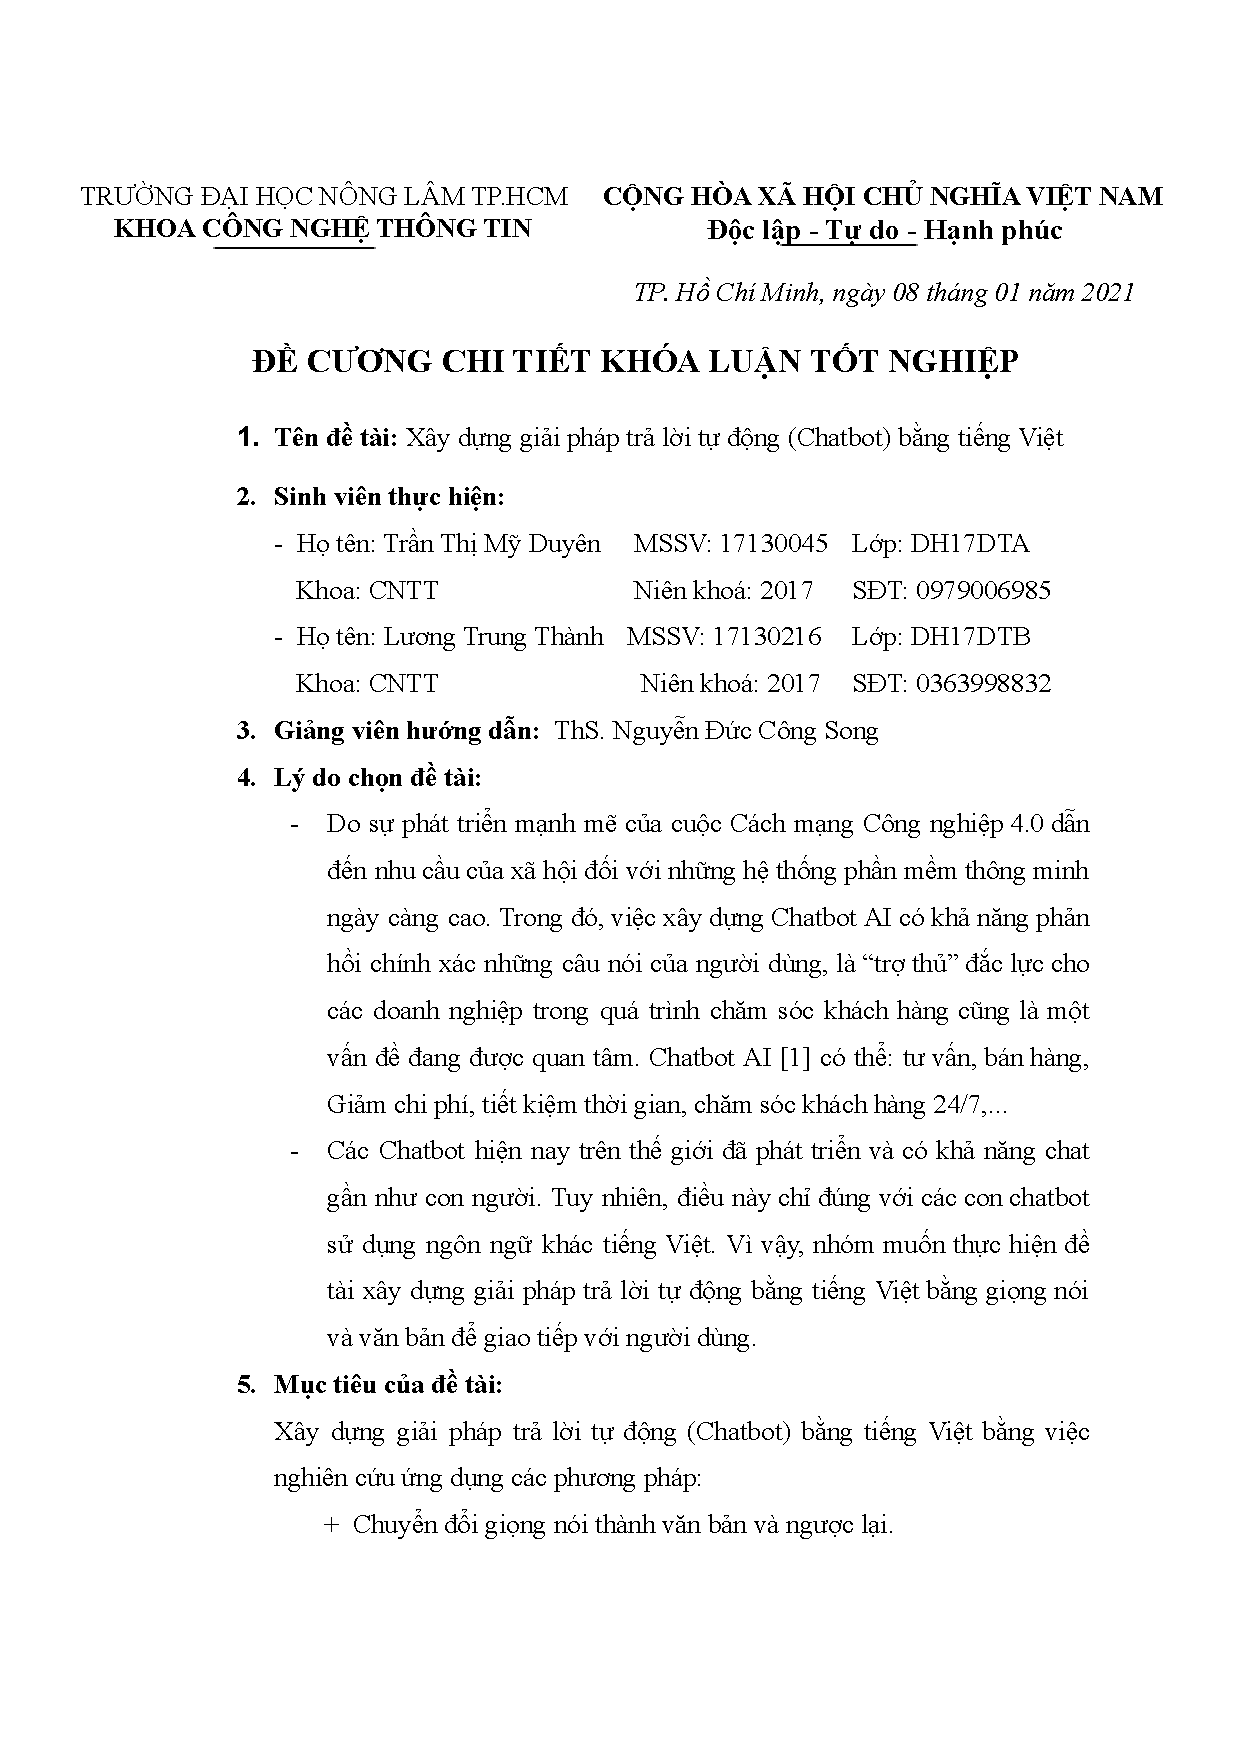
\includepdf[page=-]{Appendix/decuong}

% Mục lục, danh sách hình, danh sách bảng
\phantomsection
\addcontentsline{toc}{chapter}{Mục lục}
\tableofcontents
\listoffigures
\listoftables
\chapter*{Bảng viết tắt}
\begin{acronym}[AAAAAAAAA]
  \acro  {api} [API]   {giao diện lập trình ứng dụng -- Application Programming Interface}
\acro  {stt} [STT]   {chuyển đổi giọng nói thành văn bản -- Speech To Text}
\acro  {tts} [TTS]   {chuyển đổi văn bản thành giọng nói -- Text To Speech}
\acro  {nlu} [NLU]   {hiểu ngôn ngữ tự nhiên -- Natural Language Understanding}
\acro  {ai}  [AI]    {Trí tuệ nhân tạo -- Artificial Intelligence}
\acro  {nlp} [NLP]    {Xử lý ngôn ngữ tự nhiên -- Natural language processing}
\acro  {ner} [NER]    {Nhận dạng thực thể -- Named Entity Recognition}
\acro  {nlg} [NLG]    {Bộ sinh ngôn ngữ tự nhiên -- Natural language generation}

\end{acronym}

\phantomsection
\addcontentsline{toc}{chapter}{Tóm tắt}
\chapter*{Tóm tắt}
\label{tomtat}
Hiện nay, các Chatbot trên thế giới đã phát triển và có khả năng chat gần như con người. Tuy nhiên, điều này chỉ đúng với các Chatbot sử dụng ngôn ngữ khác tiếng Việt. Vì vậy, nhóm chúng em muốn thực hiện đề tài xây dựng giải pháp trả lời tự động bằng tiếng Việt bằng giọng nói và văn bản để giao tiếp với người dùng. Để thực hiện mục tiêu này, nhóm chúng em đã nghiên cứu về cách xây dựng Chatbot với \ac{nlu}, sau đó sử dụng các thuật toán và \ac{api} có sẵn để phân tích, trích xuất nội dung để có thể hiểu câu hỏi và tìm kiếm câu trả lời phù hợp. Nhóm đã quyết định xây dựng một ứng dụng Chatbot trên thiết bị di động, với chủ đề là các vấn đề về hướng dẫn đường đi, khoảng cách, vị trí,... Sau sáu tháng nghiên cứu và xây dựng, nhóm chúng em đã căn bản xây dựng thành công hệ thống này bao gồm ứng dụng chatbot trên thiết bị di động với dữ liệu đầu vào và kết quả đầu ra khi chat là cả giọng nói (audio) và văn bản (text) với ngôn ngữ sử dụng là tiếng Việt, tạo một bộ dữ liệu huấn luyện Chatbot. Trong đó, sử dụng thư viện SpeechToText\cite{stt} và TTSpeech\cite{tts} để chuyển đổi giọng nói thành văn bản và ngược lại. Nghiên cứu bộ thư viện Snips NLU\cite{Snipsnlu} - mã nguồn mở để phân tích ý định và trích xuất nội dung. Từ đó, sử dụng Google Map API\cite{ggmaps} để tìm kiếm các phản hồi phù hợp (Search compatible response). Tạo một bộ dữ liệu dùng để huấn luyện bằng tiếng Việt và thực hiện dịch (translate) từ tiếng Việt sang tiếng Anh bằng bộ từ điển kết hợp với sử dụng thư viện VNCoreNLU\cite{vncorenlu} để kết quả dịch chính xác hơn. Tuy nhiên, sản phẩm vẫn còn điểm yếu là độ chính xác chưa cao (90\%), bộ dữ liệu huấn luyện còn đơn giản (80 câu huấn luyện và 40 câu kiểm thử) với 4 loại ý định thuộc lĩnh vực hỏi đường đi trong phạm vi Thành phố Thủ Đức. Nhóm chúng em sẽ tiếp tục nghiên cứu và hoàn thiện hơn sản phẩm trong thời gian sắp tới. 


\clearpage

\pagenumbering{arabic} % Đánh số 1, 2, 3, ...

% Các chương nội dung
\chapter{Tổng quan}
\label{Chapter1}

\emph{Chương này trình bày sơ lược về đề tài, mục tiêu và kết quả đề tài.}

\section{Đặt vấn đề}

Với sự phát triển mạnh mẽ của cuộc cách mạng công nghiệp 4.0 dẫn đến nhu cầu xã hội đối với những phần mềm thông minh ngày càng cao. Trong thời gian gần đây, việc thiết kế và triển khai Chatbots đã nhận được sự quan tâm rất lớn của các nhà phát triển và các nhà nghiên cứu. Chatbots là hệ thống hội thoại dựa trên \ac{ai} có thể xử lý ngôn ngữ của con người thông qua các kỹ thuật khác nhau bao gồm \ac{nlp} và Mạng thần kinh (NN). Hàng loạt các thuật toán ra đời giúp cho Chatbots ngày càng thông minh và chính xác hơn.

Hiện nay, Chatbots đã được áp dụng trên rất nhiều lĩnh vực như:
\begin{itemize}
    \item[--] Giải trí: Người dùng có thể nói chuyện và tương tác với chúng mọi lúc mọi nơi, nó trả lời câu hỏi của bạn theo cách nhân văn nhất và có thể hiểu được tâm trạng của bạn với ngôn ngữ mà bạn đang sử dụng. Các Chatbots giải trí trực tuyến như là: Mitsuku, Rose, Insomno Bot,...
    \item[--] Thời tiết: Được thiết kế như một chuyên gia dự báo thời tiết và cảnh báo thời tiết xấu đối với người dùng như là Chatbot Poncho.
    \item[--] Y tế: Chatbot này sẽ hỏi về các triệu chứng, các thông số cơ bản và lịch sử y tế, sau đó biên soạn ra một danh sách các nguyên nhân gây ra cũng như các loại bệnh có thể mắc phải theo thứ tự nghiêm trọng.
    \item[--] Khách sạn và du lịch: Đây là một loại Chatbot khá phổ biến và được sử dụng một cách rộng rãi giúp tiết kiệm thời gian và giảm chi phí nhân lực. Chúng được lập trình để có thể trò chuyện cùng khách hàng và nhờ đó có thể biết được các mong muốn và yêu cầu của khách hàng một cách đơn giản hơn.
\end{itemize}

Các Chatbots hiện nay trên thế giới đã phát triển gần như là con người. Tuy nhiên điều này thường đúng với các Chatbot sử dụng ngôn ngữ khác tiếng Việt. Vì vậy, nhóm chúng em muốn thực hiện đề tài xây dựng Chatbots với ngôn ngữ tiếng Việt bằng giọng nói và văn bản để giao tiếp với con người.

\section{Mục tiêu}

Nghiên cứu các thành phần cấu tạo Chatbots. Tìm hiểu các kỹ thuật xử lý ngôn ngữ trong \ac{nlu} như phân loại ý định (intent classification hay intent detection), trích xuất thông tin (information extraction),.. trong việc xây dựng Chatbots.

Luận văn tập trung tìm cách giải quyết các bài toán mà chatbot ứng dụng trong miền đóng (Closes domain: các cuộc hội thoại tập trung vào một miền cụ thể như y tế, du lịch,...) và trả lời theo mô hình truy xuất thông tin (retrieval-based). Mô hình truy xuất thông tin là mô hình trong đó, chatbot đưa ra những phản hồi được chuẩn bị trước hoặc tuân theo những mô thức nhất định. Mô hình này khác với mô hình tự động sinh câu trả lời (generative), trong đó câu trả lời của chatbot được tự động sinh ra bằng việc học từ một tập dữ liệu. Các hệ thống chatbot được triển khai trong thực tế phần lớn tuân theo mô hình truy xuất thông tin và được áp dụng trong những miền ứng dụng nhất định.

Với đề tài này, chúng em sẽ tập trung xây dựng giải pháp trả lời tự động (Chatbots) bằng tiếng Việt trong lĩnh vực hỏi đường dựa nào Snips-NLU và áp dụng những kiến thức tìm hiểu về chatbot để có thể tuỳ chỉnh trên mã nguồn mở này. Đối tượng người dùng chatbot cụ thể ở đây là những người có nhu cầu sử dụng ứng dụng để chỉ đường đi.

\section{Kết quả}
Xây dựng giải pháp trả lời tự động (Chatbots) bằng tiếng Việt với các chức năng sau:
\begin{itemize}
    \item[--] Ứng dụng chatbot (xác định ý định và trích xuất thông tin).
    \item[--] Sử dụng ngôn ngữ trò chuyện chính là Tiếng Việt.
    \item[--] Cho phép người dùng cuối tương tác với chatbot bằng giọng nói và văn bản.
    \item[--] Bộ dữ liệu dùng để huấn luyện, tài liệu đầu vào mẫu và phương pháp giải quyết các vấn đề về câu trả lời phản hồi.
    \item[--] Ứng dụng kết hợp với bản đồ hướng dẫn đường đi.
\end{itemize}



Cuốn luận được trình bày theo cấu trúc sau:
\begin{itemize}
    \item Chương 1: Giới thiệu: Sơ lược về đề tài, mục tiêu, cách tiếp cận và kết quả đề tài, cấu trúc cuốn luận
    \item Chương 2: Các hệ thống và thuật toán liên quan
          \begin{itemize}
              \item Giới thiệu Chatbots
              \item Các hệ thống tương tự
              \item Một số phương pháp hiểu ngôn ngữ tự nhiên - (\ac{nlu})
          \end{itemize}
    \item Chương 3: Giải pháp và phương án thực hiện
          \begin{itemize}
              \item Hiểu ngôn ngữ tự nhiên (\ac{nlu})
              \item Xác định Intent
              \item Trích xuất thông tin (Filling slots)
              \item Giải pháp xây dựng ứng dụng
              \item Kết quả lựa chọn công nghệ
          \end{itemize}
    \item Chương 4: Triển khai ứng dụng
          \begin{itemize}
              \item Phân tích, đặc tả bài toán: Trình bày các phân tích về bài toán, từ đó đưa ra cái nhìn tổng quan về hệ thống sẽ xây dựng
              \item Thiết kế kiến trúc hệ thống: Sơ đồ và diễn giải thiết và phần mềm của bài toán
              \item Thiết kế giao diện ứng dụng
          \end{itemize}
    \item Chương 5: Kết quả: Trình bày kết quả lựa chọn thuật toán, công nghệ, và các thiết kế chi tiết của hệ thống
          \begin{itemize}
              \item Một số chức năng đã cài đặt
          \end{itemize}
    \item Chương 6: Kết luận và hướng phát triển: Trình bày kết luận đề tài và hướng phát triển về sau
          \begin{itemize}
              \item Kết luận đề tài
              \item Hướng phát triển
          \end{itemize}
\end{itemize}

\chapter{Các hệ thống và thuật toán liên quan}
\label{Chapter2}

\emph{Chương này giới thiệu về một số hệ thống tương tự với hệ thống chỉ đường cũng như một số thuật toán xử lí giọng nói.}

\section{Giới thiệu về chatbot}
	Chatbot là một chương trình máy tính được xây dựng để có thể trò chuyện với con người. Một chat-bot đơn giản có thể dùng để thay con người trả lời các câu hỏi lặp đi lặp lại của người dùng như: “Sự kiện X diễn ra khi nào?”, “Vinaphone MAX70 là gì?”, “iPhone X giá bao nhiêu?”,… Chatbot cũng có thể đóng vai trò là một trợ lý ảo, trợ giúp trong các công việc phức tạp hơn như hỗ trợ đặt hàng, đăng ký một sự kiện, hoành thành các biểu mẫu,… hầu hết các công việc/hoặc tác vụ có thể được thực hiện theo các bước.

Ưu điểm của chatbot
\begin{itemize}
    \item 1. Cung cấp dịch vụ khách hàng nhanh chóng hơn
          \begin{itemize}
              \item Phần mềm này hỗ trợ doanh nghiệp cung cấp dịch vụ khách hàng 24 giờ/ngày, bất kể cuối tuần hay nghỉ lễ.
              \item Khi khách hàng trực tuyến có thắc mắc, họ chỉ cần hỏi trong chatbot trên trang web của bạn mà không cần phải chờ đợi lâu để có câu trả lời. Bởi câu trả lời chỉ là một vài tổ hợp được lập trình sẵn.
          \end{itemize}
    \item 2. Làm tăng sự hài lòng của khách hàng
          \begin{itemize}
              \item Khi khách hàng nhận được câu trả lời thỏa đáng với dịch vụ nhanh chóng nhờ chatbot, họ sẽ cảm thấy hài lòng hơn và tiếp tục mua sản phẩm của bạn.
          \end{itemize}
    \item 3. Giảm chi phí lao động
          \begin{itemize}
              \item Chatbot giúp bạn giữ chi phí kinh doanh thấp bởi số tiền bạn đầu tư vào chatbot ít hơn số tiền bạn phải trả cho nhân viên.
              \item Bằng cách này, bạn thực sự tiết kiệm được rất nhiều tiền thay vì việc duy trì một trung tâm hỗ trợ khách hàng. Tính năng này sẽ giúp bạn tiết kiệm tài chính, tránh những rắc rối trong quản lý nhân sự, và tiết kiệm thời gian để làm những việc cần thiết khác.
          \end{itemize}
    \item 4. Nhiều mục đích sử dụng
          \begin{itemize}
              \item Bạn có thể sử dụng chatbot trong nhiều mảng, ví dụ như nhận đơn đặt hàng của khách, dịch vụ khách hàng và quảng cáo sản phẩm.
            
          \end{itemize}
         
              
\end{itemize}
   \begin{figure}[htp]
              \centering
              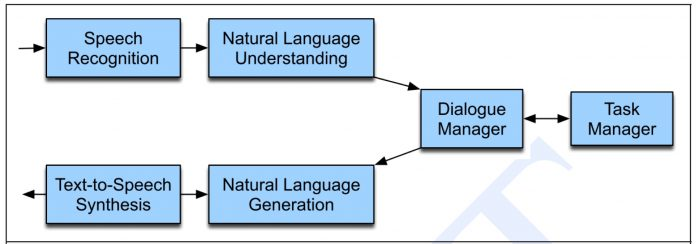
\includegraphics[width=10cm]{images/k.jpg} 
              \caption{Kiến trúc cơ bản của một hệ thống giao tiếp tự động}
              \label{fig:system-class-intent}
          \end{figure}


	Các hệ thống chatbot giao tiếp với con người bằng giọng nói (như Siri) hoặc bằng văn bản (như các chatbot phát triển trên nền Facebook Messenger). Dù giao tiếp bằng hình thức nào, chatbot cũng cần phải hiểu văn bản để có thể đưa ra những câu trả lời phù hợp cho khách hàng. Thành phần đảm nhiệm công việc này trong hệ thống chatbot được gọi là NLU (Natural Language Understanding), trong đó có rất nhiều các kĩ thuật xử lý ngôn ngữ tự nhiên (Natural Language Processing, viết tắt là NLP) được áp dụng.
\\
	Hai thành phần liên quan đến xử lý ngôn ngữ tự nhiên không thể thiếu của một NLU module là bộ phân loại ý định và nhận diện thực thể (NER). Phân loại ý định giúp chat-bot hiểu ý định của người dùng. Về mặt bản chất phân loại ý định chính là một bài toán phân loại câu với tập nhãn là các ý định có thể có của người dùng (đã được định nghĩa từ trước). NER giúp chat-bot trích xuất các thông tin trong yêu cầu/câu trả lời của người dùng. Các thông tin đó có thể là tên sản phẩm, địa chỉ, số điện thoại, số tài khoản của người dùng,… NER là một bài toán gán nhãn chuỗi cơ bản: cho vào một câu đầu vào, trích xuất tất cả các thực thể định danh trong câu và phân loại chúng vào một trong các nhãn đã được định nghĩa từ trước.
\\
	Một thành phần xử lý ngôn ngữ tự nhiên khác có thể được thêm vào chat-bot là bộ quản lý hội thoại, bộ sinh ngôn ngữ (NLG), và bộ phân tích cảm xúc. Một bộ quản lý hội thoại sẽ lưu trữ, phân tích và tận dụng ngữ cảnh cuộc hội thoại và giúp chat-bot suy luận hành động tiếp theo trong khi NLG giúp sinh câu trả lời đầy đủ, tự nhiên nhất bằng ngôn ngữ tự nhiên cho chat-bot. Một bộ phân tích cảm xúc có thể cần bởi vì cùng một câu có thể mang nhiều nghĩa khác nhau trong các văn cảnh khác nhau, do đó có thể cần được trả lời theo các cách khác nhau phụ thuộc vào cảm xúc của người dùng.
\\
	Bài luận này chủ yếu nghiên cứu về phát hiện ý định và trích xuất thực thể trong NLU module.

\section{Một số hệ thống hiểu ngôn ngữ tự nhiên}

\subsection{Giới thiệu về hiểu ngôn ngữ tự nhiên}

	Hiểu ngôn ngữ tự nhiên là một chủ đề của xử lý ngôn ngữ tự nhiên trong lĩnh vực trí tuệ nhân tạo. Để có thể xây dựng một chatbot hoặc trợ lý giọng nói thì điều không thể thiếu đó chính là hiểu được ngôn ngữ tự nhiên.

	Bất cứ khi nào người dùng tương tác với AI bằng ngôn ngữ tự nhiên, các từ của họ cần phải được dịch thành một mô tả mà máy có thể đọc được về ý của họ.
Công cụ \ac{nlu} trước tiên phát hiện ý định của người dùng là gì (intent), sau đó trích xuất các tham số (slot) của truy vấn. Sau đó, nhà phát triển có thể sử dụng điều này để xác định hành động hoặc phản hồi thích hợp.

Các khái niệm cơ bản:
\begin{itemize}
    \item 1.Xác định ý định người dùng
    \\
          Thông thường, người dùng thường truy cập hệ thống chatbot với mong muốn hệ thống sẽ đưa ra những hành động trợ giúp mình về một vấn đề nào đó. Ví dụ, người dùng của hệ thống chatbot hỗ trợ đặt vé máy bay có thể đưa ra yêu cầu đặt vé của mình khi bắt đầu cuộc hội thoại. Để đưa ra hỗ trợ được chính xác, chatbot cần xác định được ý định (intent) đó của người dùng. Việc xác định ý định của người dùng sẽ quyết định hội thoại tiếp theo giữa người và chatbot sẽ diễn ra như thế nào. Vì thế, nếu xác định sai ý định người dùng, chatbot sẽ đưa ra những phản hồi không đúng, không hợp ngữ cảnh. Khi đó, người dùng có thể thấy chán ghét và không quay lại sử dụng hệ thống. Bài toán xác định ý định người dùng vì thế đóng vai trò rất quan trọng trong hệ thống chatbot.
          \\
          Đối với miền ứng dụng đóng, chúng ta có thể giới hạn rằng số lượng ý định của người dùng nằm trong một tập hữu hạn những intent đã được định nghĩa sẵn, có liên quan đến những nghiệp vụ doanh nghiệp mà chatbot có thể hỗ trợ. Với giới hạn này, bài toán xác định ý định người dùng có thể quy về bài toán phân lớp văn bản. Với đầu vào là một câu giao tiếp của người dùng, hệ thống phân lớp sẽ xác định intent tương ứng với câu đó trong tập các intent đã được định nghĩa.
    \item 2. Trích xuất thông tin
    \\
          Bên cạnh việc xác định intent trong câu hội thoại của người dùng, chúng ta cần trích xuất các thông tin cần thiết trong đó. Các thông tin cần trích xuất trong một câu hội thoại thường là các thực thể thuộc về một loại nào đó. Ví dụ, khi một khách hàng muốn đặt vé máy bay, hệ thống cần biết địa điểm xuất phát và địa điểm khách muốn đến, ngày giờ khách hàng muốn bay,…Thành phần NLU của các hệ thống chatbot thường hỗ trợ các loại thực thể sau (tham khảo tài liệu [2]):
          \\
          Vị trí (Location)
          \\
          	Thời gian (Datetime)
          \\
         	 Số (Number)
          \\
         	 Địa chỉ liên lạc (Contact)
          \\
         	 Khoảng cách (Distance)
          \\
          	Khoảng thời gian (Duration)
          \\
          Đầu vào của một module trích xuất thông tin là một câu hội thoại. Module trích xuất thông tin cần xác định vị trí của các thực thể trong câu (vị trí bắt đầu và vị trí kết thúc của thực thể). Ví dụ sau minh hoạ một câu hội thoại và các thực thể được trích xuất từ đó.
          \\
          Câu hội thoại: Tôi muốn đặt vé máy bay đi Phú Quốc từ sân bay Nội Bài lúc 8 giờ tối ngày mai.
          \\
          Câu có các thực thể được xác định: Tôi muốn đặt vé máy bay đi [Phú Quốc]LOCATION từ sân bay [Nội Bài]LOCATION lúc [8 giờ tối ngày mai]TIME.
          \\
          Trong câu trên có 3 thực thể (nằm trong các dấu [ ]) với các loại thực thể tương ứng (được viết với font chữ nhỏ hơn ở dưới).
\end{itemize}
\subsection{Lựa chọn thuật toán}

\begin{itemize}
    \item 1. Xác định intent
          Để xây dựng một mô hình phân lớp intent, chúng ta cần một tập dữ liệu huấn luyện bao gồm các cách diễn đạt khác nhau cho mỗi intent. Ví dụ, cùng một mục đích hỏi về thời tiết ở Hà Nội trong ngày hôm nay, người dùng có thể dùng những cách diễn đạt sau:
          Thời tiết hôm nay ở Hà Nội thế nào ad?
          Hà Nội hôm nay có mưa không vậy?
          Hà Nội hôm nay bao nhiêu độ vậy?
          Cho mình hỏi, ra ngoài đường hôm nay có phải mang áo mưa không?
          Có thể nói, bước tạo dữ liệu huấn luyện cho bài toán phân lớp intent là một trong những công việc quan trọng nhất khi phát triển hệ thống chatbot và ảnh hưởng lớn tới chất lượng sản phẩm của hệ thống chatbot về sau. Công việc này cũng đòi hỏi thời gian, công sức khá lớn của nhà phát triển chatbot.
          Mô hình học máy cho bài toán phân lớp ý định người dùng
          Khi đã có dữ liệu huấn luyện cho bài toán phân lớp intent, chúng ta sẽ mô hình bài toán thành bài toán phân lớp văn bản. Bài toán phân lớp văn bản (text categorization) là một bài toán kinh điển trong ngành NLP và khai phá văn bản (Text Mining). Mô hình phân lớp văn bản cho bài toán phân lớp intent được phát biểu một cách hình thức như sau:
          Chúng ta được cho trước một tập huấn luyện bao gồm các cặp (câu hội thoại, intent), D = {(x(1), y(1)),…, (x(n), y(n))}, trong đó x(i) là các câu hội thoại và y(i) là intent tương ứng cho x(i). Các intent y(i) nằm trong một tập hữu hạn .... các intent được định nghĩa trước. Chúng ta cần học từ tập huấn luyện này một mô hình phân lớp .... có chức năng phân lớp một câu hội thoại mới vào một trong các intent thuộc tập K. Kiến trúc của hệ thống phân lớp intent được minh hoạ trong hình 1.
          \begin{figure}[htp]
              \centering
              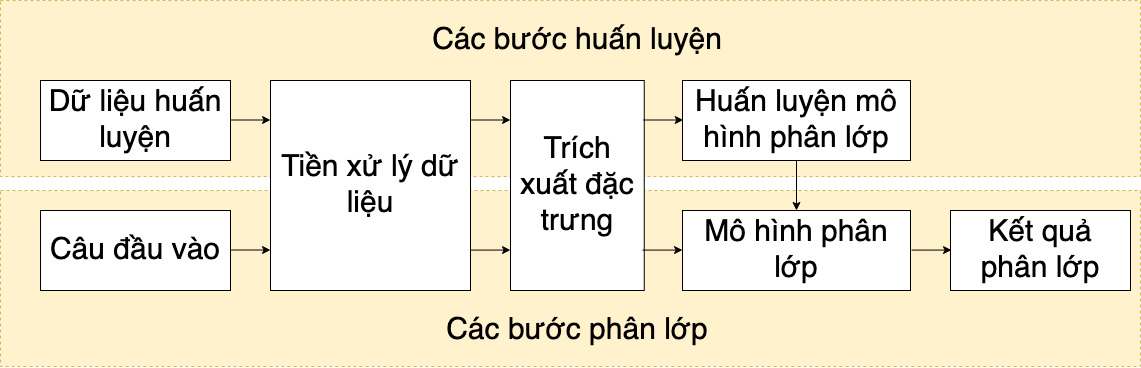
\includegraphics[width=10cm]{images/structure-system-class-intent.png}
              \caption{Kiến trúc của hệ thống phân lớp intent}
              \label{fig:system-class-intent}
          \end{figure}
          Hệ thống phân lớp intent có một số thành phần cơ bản:
          Tiền xử lý dữ liệu
          Trích xuất đặc trưng
          Huấn luyện mô hình
          Phân lớp
          Trong bước tiền xử lý dữ liệu, chúng ta sẽ thực hiện các thao tác “làm sạch” dữ liệu như: loại bỏ các thông tin dư thừa, chuẩn hoá dữ liệu như chuyển các từ viết sai chính tả thành đúng chính tả, chuẩn hoá các từ viết tắt,… Việc tiền xử lý dữ liệu có vai trò quan trọng trong hệ thống chatbot do đặc thù của ngôn ngữ chat, nói: viết tắt, sai chính tả, hay dùng “teencode”.
          Sau khi tiền xử lý dữ liệu và thu được dữ liệu đã được làm sạch, chúng ta sẽ trích xuất những đặc trưng từ dữ liệu này. Trong học máy, bước này được gọi là trích xuất đặc trưng (feature extraction hay feature engineering). Trong mô hình học máy truyền thống (trước khi mô hình học sâu được áp dụng rộng rãi), bước trích xuất đặc trưng ảnh hưởng lớn đến độ chính xác của mô hình phân lớp. Để trích xuất được những đặc trưng tốt, chúng ta cần phân tích dữ liệu khá tỉ mỉ và cần cả những tri thức chuyên gia trong từng miền ứng dụng cụ thể.
          Bước huấn luyện mô hình nhận đầu vào là các đặc trưng đã được trích xuất và áp dụng các thuật toán học máy để học ra một mô hình phân lớp. Các mô hình phân lớp có thể là các luật phân lớp (nếu sử dụng decision tree) hoặc là các vector trọng số tương ứng với các đặc trưng được trích xuất (như trong các mô hình logistic regression, SVM, hay mạng Neural).
          Sau khi có một mô hình phân lớp intent, chúng ta có thể sử dụng nó để phân lớp một câu hội thoại mới. Câu hội thoại này cũng đi qua các bước tiền xử lý và trích xuất đặc trưng, sau đó mô hình phân lớp sẽ xác định “điểm số” cho từng intent trong tập các intent và đưa ra intent có điểm cao nhất.

    \item 2. Trích xuất thông tin
          Cách tiếp cận phổ biến cho bài toán trích xuất thông tin là mô hình hoá bài toán thành bài toán gán nhãn chuỗi (sequence labeling). Đầu vào của bài toán gán nhãn chuỗi là một dãy các từ, và đầu ra là một dãy các nhãn tương ứng các các từ trong đầu vào. Chúng ta sẽ sử dụng các mô hình học máy để học một mô hình gán nhãn từ một tập dữ liệu đầu vào bao gồm các cặp (x1…xn, y1…yn), trong đó x1…xn là dãy các từ, y1…ynlà dãy các nhãn. Độ dài của các dãy từ trong tập dữ liệu có thể khác nhau.
          Trong bài toán trích xuất thông tin, tập nhãn cho các từ trong câu đầu vào thường được tạo ra theo  mô hình BIO, với B là viết tắt của “Beginning”, I là viết tắt của “Inside”, và O là viết tắt của “Outside”. Khi biết vị trí từ bắt đầu của một thực thể và các từ nằm trong thực thể đó, chúng ta có thể xác định vị trí của thực thể trong câu. Trong ví dụ ở trên, dãy các nhãn tương ứng với dãy của các từ trong câu hội thoại đầu vào được minh hoạ ở hình 2.
          Thuật toán huấn luyện mô hình gán nhãn chuỗi phổ biến là mô hình Markov ẩn (HMM – Hidden Markov Models) [3], mô hình CRF (Conditional Random Fields) [4]. Với dữ liệu văn bản, mô hình CRF thường cho kết quả tốt hơn mô hình HMM. Có khá nhiều các công cụ mã nguồn mở cài đặt mô hình CRF cho bài toán gán nhãn chuỗi như CRF++ [5], CRF Suite [6], Mallet [7],…
\end{itemize}
\begin{figure}[htp]
    \centering
    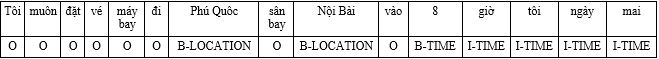
\includegraphics[width=10cm]{images/Model-BIO.png}
    \caption{Gán nhãn từ theo mô hình B-I-O trong trích xuất thông tin}
    \label{fig:model-BIO}
\end{figure}

\subsection{Một số phương pháp hiểu ngôn ngữ tự nhiên}

\begin{itemize}
    \item Rasa \ac{nlu}
          \begin{figure}[htp]
              \centering
              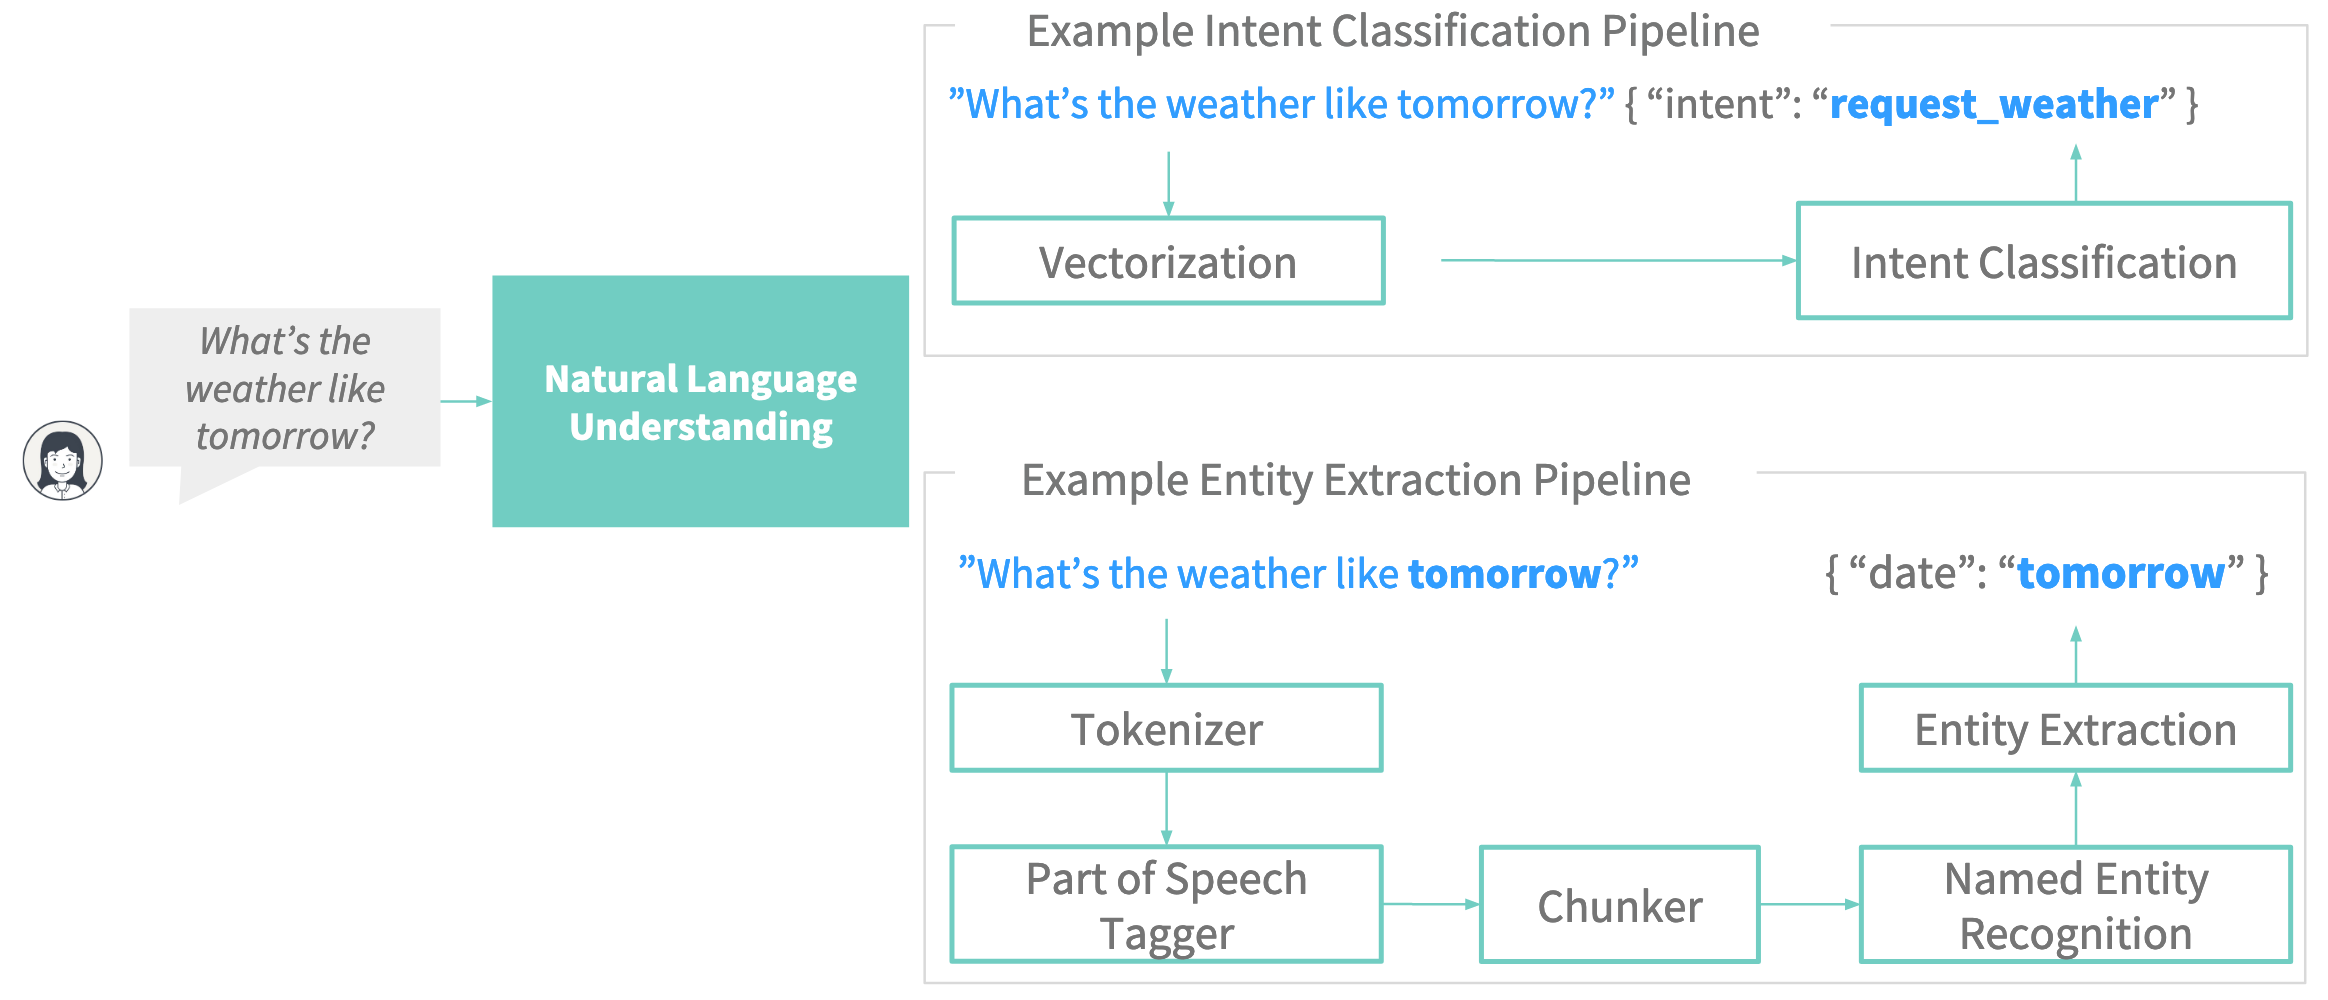
\includegraphics[width=10cm]{images/Rasa-NLU.png}
              \caption{Sơ đồ hệ thống Rasa-\ac{nlu}}
              \label{fig:rasa-nlu}
          \end{figure}
    \item Snips \ac{nlu}
          \begin{figure}[htp]
              \centering
              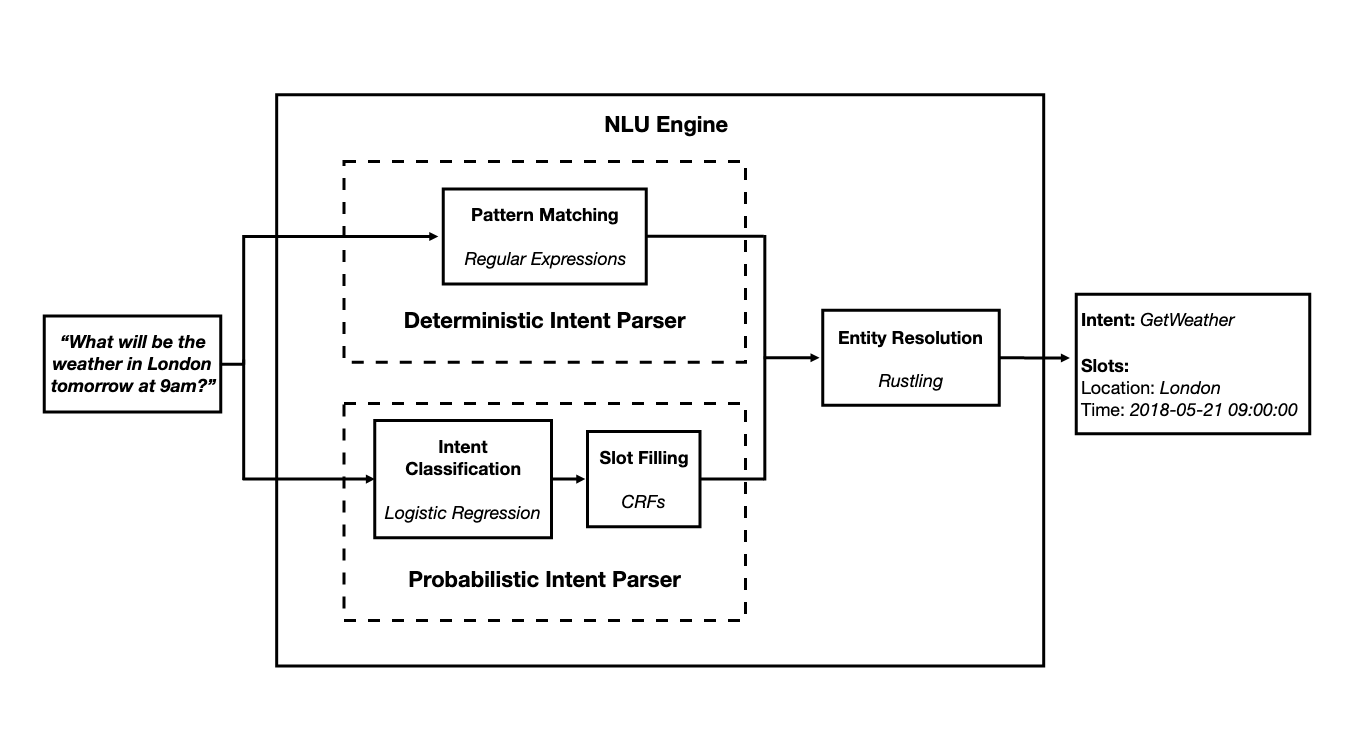
\includegraphics[width=10cm]{images/Snips-NLU.png}
              \caption{Sơ đồ hệ thống Snips-\ac{nlu}}
              \label{fig:snips-nlu}
          \end{figure}
          Có thể khái quát các luồng xử lý của snips-NLU \cite{snips-nlu} như sau:
          Hệ thống Snips-NLU (hình \ref{fig:snips-nlu}) chứa một thành phần chính, NLU Engine, bản thân nó bao gồm một số thành phần sau:
          \begin{itemize}
              \item Deterministic intent parser: Mục tiêu của trình phân tích cú pháp xác định là cung cấp độ mạnh mẽ và trải nghiệm có thể dự đoán được cho người dùng vì nó được đảm bảo đạt được 1.0 F1-Score trên các ví dụ đào tạo. Các truy vấn có trong dữ liệu huấn luyện được sử dụng để xây dựng các mẫu bao gồm tất cả các tổ hợp giá trị thực thể.
              \item Probabilistic intent parser: Trình phân tích cú pháp mục đích nhằm mục đích mở rộng phân tích cú pháp vượt ra ngoài các ví dụ đào tạo và nhận ra các biến thể không xuất hiện trong dữ liệu đào tạo. Nó cung cấp sức mạnh tổng quát hóa mà trình phân tích cú pháp xác định thiếu. Thông qua hai bước intent classification (xác định ý định) and slot filling (trích xuất thực thể).
              \item Entity resolution:
          \end{itemize}
\end{itemize}
Trong bài luận này em sử dụng Snips NLU cho việc xác định intent vì:
\begin{itemize}
    \item Miễn phí vì nó là opensource
    \item Gọn nhẹ và dễ dàng sử dụng vì có cộng đồng lớn
    \item Hiệu suất cao.
\end{itemize}
Trong hình dưới đây, điểm F1 của cả phân loại ý định và trích xuất slot đã được tính toán cho một số nhà cung cấp NLU và được tính trung bình trên ba bộ dữ liệu Lights dataset\footnote{Xem thêm về Lights dataset tại đây:\url{https://github.com/snipsco/snips-nlu/blob/master/sample_datasets/lights_dataset.json}}, Beverage dataset\footnote{Xem thêm về Beverage dataset tại đây:\url{https://github.com/snipsco/snips-nlu/blob/master/sample_datasets/beverage_dataset.json}}, Flights dataset\footnote{Xem thêm về Flights dataset tại đây:\url{https://github.com/snipsco/snips-nlu/blob/master/sample_datasets/flights_dataset.json}}
\begin{figure}[htp]
    \centering
    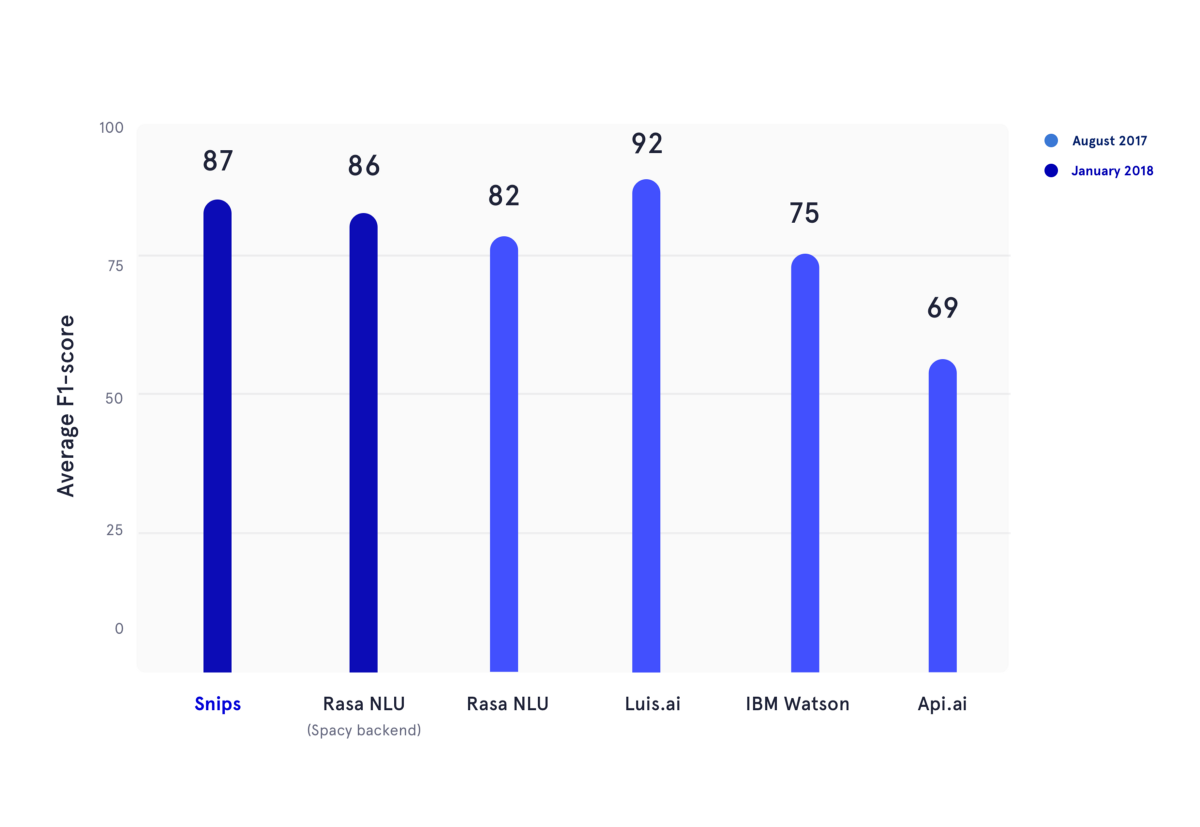
\includegraphics[width=10cm]{images/benchmarks.png}
    \caption{Bảng so sánh}
    \label{fig:benchmarks}
\end{figure}

\chapter{Nghiên cứu hệ thống chỉ đường}
\label{Chapter3}

\emph{Chương này sẽ trình bày, mô tả chi tiết về các nghiên cứu đã được thực hiện để giải quyết bài toán chỉ đường, bao gồm danh sách và việc lựa chọn một số thuật toán xử lí giọng nói}

\section{Giới thiệu}
\begin{figure}[htp]
    \centering
    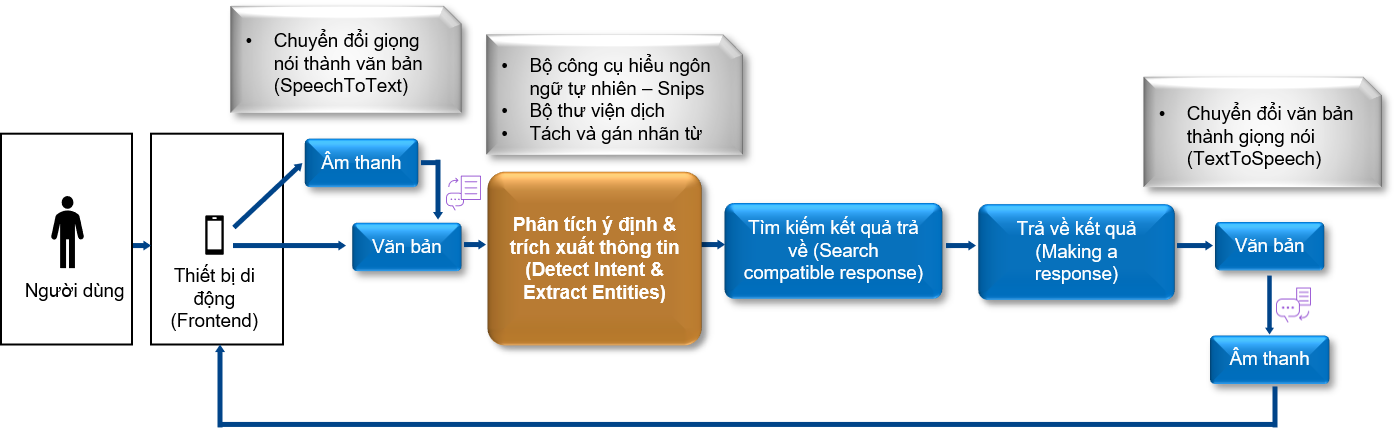
\includegraphics[width=10cm]{images/Structure-description.png}
    \caption{Sơ đồ của hệ thống chỉ đường}
    \label{fig:sodohethongchiduong}

\end{figure}

Khi người dùng sử dụng ứng dụng di động gửi một câu truy vấn bằng audio thì ứng dụng di động sẽ chuyển giọng nói đó thành văn bản (speech to text)

Văn bản đó được gửi tới NLU engine để trích xuất ý định và các thực thể

Dựa trên ý định và thực thể nhận được, hệ thống sẽ truy vấn dữ liệu thông qua google API, tạo ra câu trả lời tương ứng và trả về cho người dùng bằng text và audio ( text to speech để chuyển văn bản thành giọng nói)

Trong phạm vi bài luận này, nhóm em nghiên cứu sử dụng công cụ có sẵn Snips NLU\cite{Snipsnlu} cho việc trích xuất ý định và các thực thể

Snips NLU là công cụ giúp hiểu ngôn ngữ tự nhiên mạnh mẽ, nhưng hiện tại chưa hỗ trợ tiếng Việt, ý tưởng của nhóm em là sẽ tạo một bộ dữ liệu bằng tiếng Việt rồi dịch sang tiếng Anh, dùng dữ liệu tiếng Anh đó để huấn luyện cho mô hình. Khi người dùng truy vấn thì dịch câu truy vấn đó sang tiếng Anh và đưa vào mô hình để trích xuất ý định và các thực thể.

Về mặt dữ liệu:
\begin{itemize}
    \item[--] Định dạng bộ dữ liệu huấn luyện là ở dạng json
    \item[--] Dữ liệu gồm 2 intent là findRoute và askLocation. Mỗi intent gồm 20 câu huấn luyện và 10 câu để kiểm thử
    \item[--] Nhóm em có viết một Script để hỗ trợ việc tạo dữ liệu trở nên đơn dễ dàng hơn.
\end{itemize}

\section{Dịch}

Đầu tiên nhóm em dịch bộ dữ liệu bằng cách tách 1 câu thành từng từ rồi sử dụng thư viện (word2word) để dịch sang tiếng Anh.Vd để dịch câu: "cách đi từ đại học Kinh Tế đến đại học Văn Lang".
\begin{itemize}
    \item[--] Tách câu thành từng từ riêng biệt: ['cách', 'đi', 'từ', 'đại', 'học', 'Kinh' ,'Tế' ,'đến', 'đại', 'học', 'Văn', 'Lang']
    \item[--] Dịch từng từ sang tiếng Anh, ta được: ['ways', 'gone', 'word', 'Swordsman', 'learn', 'GrosDs', 'Monk', 'until', 'Swordsman', 'learn', 'Lam', 'Lang']
\end{itemize}
Sau khi dịch ta được bộ dữ liệu huấn luyện\footnote{Xem thêm về bộ huấn luyện \url{https://drive.google.com/file/d/1yoQk3AuViJpkcDQumQI-SbIw_iGyaGoJ/view?usp=sharing}} và bộ dữ liệu kiểm thử\footnote{Xem thêm về bộ kiểm thử \url{https://drive.google.com/file/d/1i2YNlvZTVsTU2WrzIMBmxl4FcJuAtVyV/view?usp=sharing}}
\begin{figure}[htp]
    \centering
    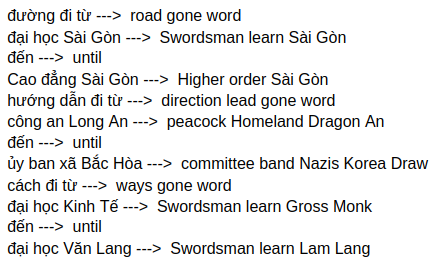
\includegraphics[width=10cm]{images/trainingdata_dichtungtu.png}
    \caption{Hình ảnh minh họa dữ liệu trước khi dịch và sau khi dịch}
    \label{fig:sodohethongchiduong}
\end{figure}

Đem bộ dữ liệu để huấn luyện và đánh giá, ta đạt được kết quả như hình 3.3, xem chi tiết \footnote{\url{https://drive.google.com/file/d/1e2Z0g4irQXqeNMzz4rP1UPQ3OKqYsMPI/view?usp=sharing}}:

\begin{figure}[htp]
    \centering
    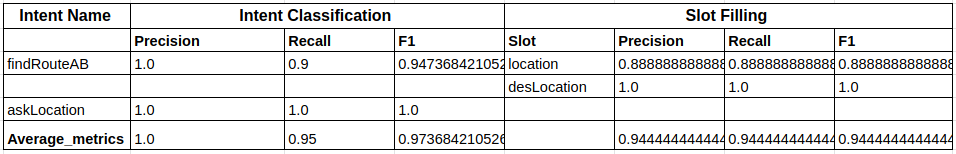
\includegraphics[width=15cm]{images/metrics-dich-tung-t.png}
    \caption{Các chỉ số của mô hình}
    \label{fig:sodohethongchiduong}
\end{figure}
Nhận xét kết quả đạt được:
\begin{itemize}
    \item[--] Mặc dù kết quả tương đối tốt nhưng phương pháp dịch từng từ này không khả thi bởi vì sẽ mà mất ý nghĩa của câu nói, ví dụ như câu sau: "từ Đại học Khoa học Tự nhiên đến Đại học Bách khoa đi như thế nào" được dịch thành "word Swordsman learn department learn itself course until Swordsman learn centurion department" Các thực thể địa điểm như "Đại học Khoa học Tự nhiên" được dịch thành "Swordsman learn department learn itself course", "Đại học Bách khoa" dịch thành "Swordsman learn centurion department"
    \item[--] Các thực thể cần được trích xuất đã bị dịch ra và không còn ý nghĩa nữa, không thể dùng để tìm kiếm địa điểm này trên Google map được.
\end{itemize}

Để xử lý vấn đề này, nhóm em sẽ thay đổi phương pháp dịch bằng cách sử dụng thư viện để tách từ (word segmentation) và gán nhãn từ loại (pos tagging)

Trong tiếng Việt, dấu cách (space) không được sử dụng như 1 kí hiệu phân tách từ, nó chỉ có ý nghĩa phân tách các âm tiết với nhau. Do đó việc tách từ sẽ giúp cho việc dịch được chính xác hơn

Về vấn đề những slot bị dịch thành tiếng Anh làm cho nó không còn ý nghĩa nữa, nhóm em nhận thấy rằng những slot này chủ yếu là danh từ, nên nhóm sẽ sử dụng pos tagging để gán nhãn từ loại, những từ nào thuộc danh từ thì sẽ không cho dịch thành tiếng Anh.

Áp dụng word segmentation và pos tagging lên bộ dữ liệu và sử dụng thư viện word2word để dịch thì đạt được bộ dữ liệu huấn luyện\footnote{\url{https://drive.google.com/file/d/1riZLV1dam9U6q5fuutBFZkzpC6IGgvbb/view?usp=sharing}} và bộ dữ iệu kiểm thử\footnote{	\url{https://drive.google.com/file/d/1Jq1x3-owrcL1TN1igPr7HFNRxTk2emW2/view?usp=sharing}
}:
\begin{figure}[htp]
    \centering
    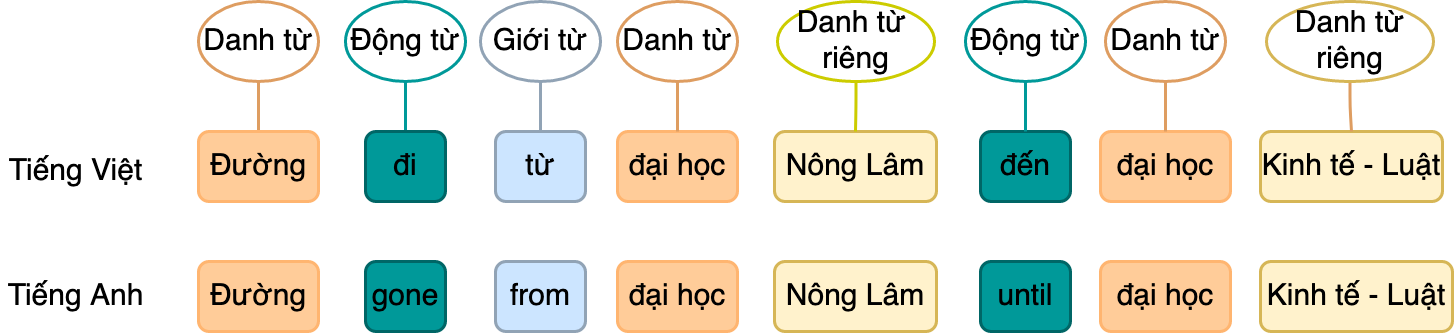
\includegraphics[width=10cm]{images/trainingdata-wordsegment.png}
    \caption{Hình ảnh minh họa dữ liệu trước khi dịch và sau khi dịch bằng phương pháp dùng word segmentation và pos tagging}
    \label{fig:sodohethongchiduong}
\end{figure}

Sau khi huấn luyện mô hình và đem đi đánh giá nhóm nhận được kết quả như  hình 3.4, xem chi tiết \footnote{\url{https://drive.google.com/file/d/1UU7_04Ps6WHZXSujZxNqaZKZhtvYsnrL/view?usp=sharing}}:

\begin{figure}[htp]
    \centering
    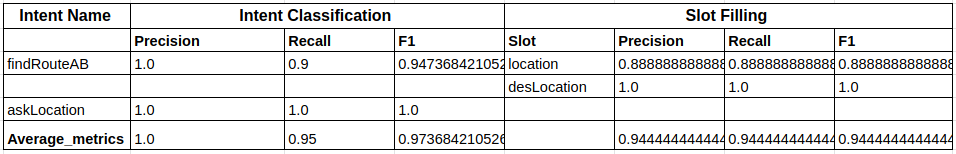
\includegraphics[width=15cm]{images/metrics-dich-tung-t.png}
    \caption{Các chỉ số của mô hình}
    \label{fig:sodohethongchiduong}

\end{figure}

Nhận xét kết quả đạt được:
\begin{itemize}
    \item[--] Sau khi áp dụng tách từ và phân loại từ vựng, nhóm đã xử lý tương đối được vấn đề dịch những slot làm mất ý nghĩa của chúng: "từ Đại học Khoa học Tự nhiên đến Đại học Bách khoa đi như thế nào" được dịch thành "word đại\_học khoa\_học\_tự\_nhiên until đại\_học bách\_khoa gone như\_thế\_nào"
\end{itemize}
Tuy nhiên vẫn còn một vài trường hợp dịch còn chưa ổn, ví dụ như "Đại học Khoa học Xã hội và Nhân văn" được dịch thành "Đại học Khoa học Xã hội their Nhân văn"

Nhóm nhận thấy rằng có thể cải thiện được bộ dịch tốt hơn, nhóm sẽ thay đổi phương pháp dịch bằng cách xây dựng một bộ từ điển, bộ từ điển này nằm trong phạm vi hỏi đường nên có thể xây dựng được, từ đó việc dịch sẽ đạt hiệu quả hơn.

Để cải thiện quá trình dịch từ tiếng Việt sang tiếng Anh, nhóm chúng em đã quyết định xây dựng bộ từ điển riêng để có thể dịch được kết quả chính xác hơn.
Trong phạm vi các câu hỏi về đường đi, chúng em đã lựa chọn dịch khoảng 50 từ và các cụm từ. Các bước để dịch được dữ liệu như sau:
\begin{itemize}
    \item[--] Bước 1: Xây dựng bộ từ điển riêng biệt về chủ đề hỏi đường đi và chuyển hoá từ ngôn ngữ tiếng Việt sang tiếng Anh.
    \item[--] Bước 2: Tìm từ dài nhất trong câu có trong bộ từ điển.
    \item[--] Bước 3: Lấy nghĩa của từ tương ứng trong từ điển.
\end{itemize}
Trong quá trình nghiên cứu, chúng em nhận thấy bước 2 là bước thật sự cần thiết để có thể tìm được từ thích hợp nhất với bộ từ điển để có kết quả tốt nhất. Dưới đây là mô tả quá trình tìm từ dài nhất có trong từ điển mà nhóm chúng em thực hiện (Xem hình Tìm từ dài nhất \ref{fig:longest-word})
\begin{itemize}
    \item[--] Input: "Đường đi từ Đại học Nông Lâm đến Ngã tư Thủ Đức""
    \item[--] Output: ["Đường đi", "từ", "Đại học Nông Lâm", "đến", "Ngã tư Thủ Đức"]
\end{itemize}
\begin{figure}[htp]
    \centering
    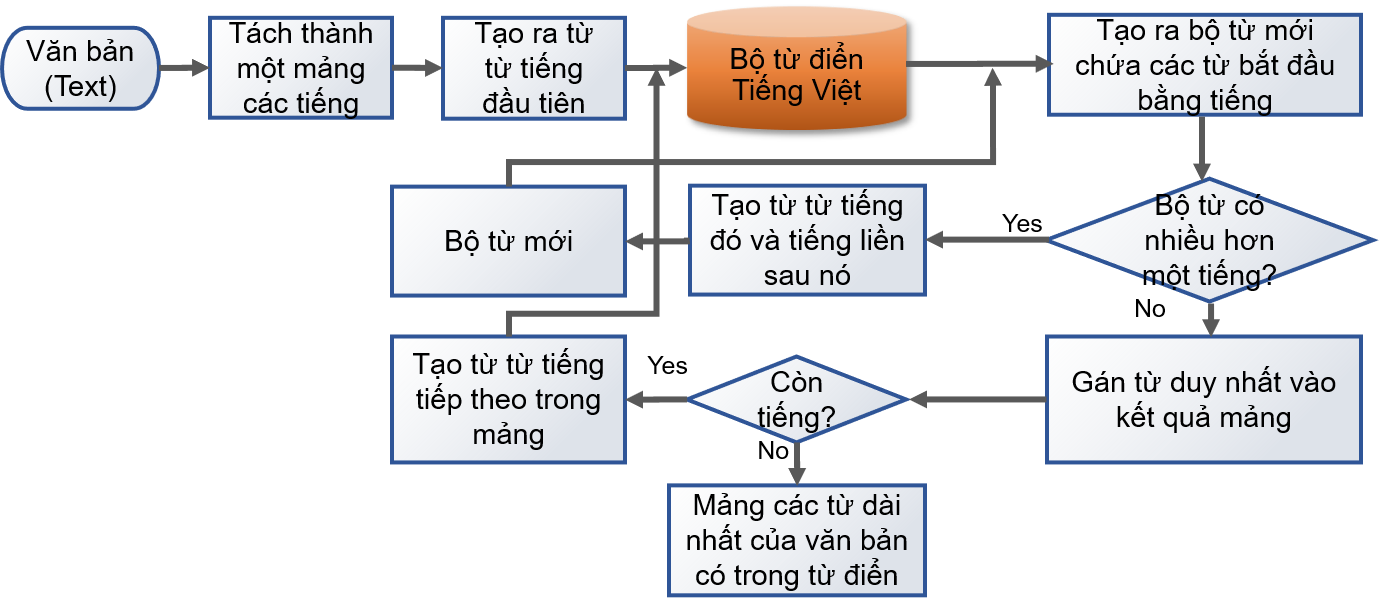
\includegraphics[width=10cm]{images/Diagram-longest-word.png}
    \caption{Tìm từ dài nhất}
    \label{fig:longest-word}
\end{figure}

Sau khi dịch ta được bộ dữ liệu huấn luyện\footnote{\url{https://drive.google.com/file/d/1l6TW8QdhZYOC7uhCpIJpsuSwVfrSv5ie/view?usp=sharing}} và bộ dữ liệu kiểm thử \footnote{\url{https://drive.google.com/file/d/1DpIxFSOjwP_djW-V1jpaLH4HTwGgGZkA/view?usp=sharing}}
\begin{figure}[htp]
    \centering
    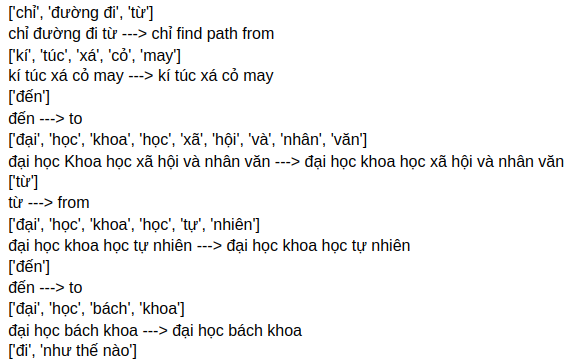
\includegraphics[width=10cm]{images/trainingdata-tudien.png}
    \caption{Hình ảnh minh họa dữ liệu trước khi dịch và sau khi dịch bằng phương pháp xây dựng từ điển}
    \label{fig:sodohethongchiduong}

\end{figure}

Đem bộ dữ liệu để huấn luyện và đánh giá, ta đạt được kết quả như hình 3.8, xem chi tiết \footnote{\url{https://drive.google.com/file/d/1HSe-ri76d8jbF3FZUCrDiFawHI17D18a/view?usp=sharing}}:

\begin{figure}[htp]
    \centering
    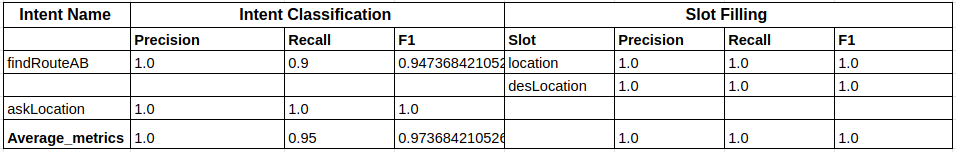
\includegraphics[width=15cm]{images/metrics-tudien.png}
    \caption{Các chỉ số của mô hình}
    \label{fig:sodohethongchiduong}
\end{figure}
Kết quả đạt được sau khi dùng phương pháp dịch bằng cách xây dựng bộ từ điển:
\begin{itemize}
    \item[--] Do xây dựng bộ từ điển những từ vựng trong phạm vi nhỏ - hỏi đường nên bộ dịch cho ra kết quả khá khả quan, cải thiện hơn so với 2 phương pháp trước là phương pháp dịch từng từ và phương pháp dịch dùng word segmentation và pos tagging
    \item[--] Kế hoạch phát triển là xây dựng thêm dữ liệu, tạo thêm nhiều ý định sau đó thực hiện đánh giá mô hình để xem mô hình có thực sự hiệu quả hay không.
\end{itemize}

\chapter{Xây dựng hệ thống chỉ đường}
\label{Chapter4}

\emph{Chương này sẽ trình bày, mô tả chi tiết về quá trình và kết quả phân tích bài toán chỉ đường, đưa ra các yêu cầu cụ thể cho bài toán. Đồng thời chương này cũng trình bày bản thế kế kiến trúc hệ thống và các thiết kế chi tiết khác.}

\section{Phân tích, đặc tả yêu cầu}

\subsection{Mô tả chung}
Viết mô tả
\subsection{Yêu cầu chức năng}

Yêu cầu chức năng 1:
\begin{itemize}
    \item[--] Dữ liệu vào: 
    \item[--] Xử lý: 
    \item[--] Kết quả: 
\end{itemize}



\subsection{Yêu cầu giao diện phần mềm}

Yêu cầu giao diện cho chức năng ... : Giao diện đơn giản, dễ sử dụng

Yêu cầu giao diện cho chức năng 1:
\begin{itemize}
    \item[--] Giao diện đơn giản, dễ sử dụng
    \item[--] yêu cầu 2
\end{itemize}

Yêu cầu giao diện cho chức năng Tương tác bằng giọng nói với một vài truy vấn đơn giản:
\begin{itemize}
    \item[--] Câu lệnh ngắn gọn, dễ đọc
    \item[--] Phản hồi ngắn gọn, dễ nghe
    \item[--] Phản hồi mọi câu lệnh dù câu lệnh đó không được hỗ trợ
    \item[--] Phải có giao diện đèn để phản hồi trực quan
\end{itemize}

\subsection{Yêu cầu hiệu suất}
\begin{itemize}
    \item[--] Thiết bị phải hoạt động được liên tục trong thời gian dài, từ 12 đến 24 giờ
    \item[--] Kết quả tạo lập biên bản phải đạt độ chính xác tối thiểu 80\%
    \item[--] Đối với chức năng tương tác bằng giọng nói, tốc độ phản hồi phải nhỏ hơn 3 giây
\end{itemize}

\subsection{Ràng buộc thiết kế}
\begin{itemize}
    \item[--] Sản phẩm phải được thiết kế bằng tiếng Việt, bao gồm giao diện người dùng, các phản hồi bằng giọng nói
    \item[--] Thiết bị phải nhỏ, gọn, có tính cơ động cao
    \item[--] Các thành phần của thiết bị phải được kết nối với nhau gọn gàng, đảm bảo tính thẩm mỹ
\end{itemize}

\subsection{Ràng buộc thuộc tính}
\begin{itemize}
    \item[--] Cơ sở dữ liệu biên bản cuộc họp phải được sao lưu thường xuyên
    \item[--] Các thành phần của thiết bị khi bị hỏng phải dễ dàng tìm kiếm và thay thế
    \item[--] Việc cập nhật phần mềm phải nhanh chóng và không gây ra mất mát dữ liệu
\end{itemize}

\section{Thiết kế kiến trúc hệ thống}

\subsection{Kiến trúc phần mềm}

\chapter{Triển khai ứng dụng}
\label{Chapter5}

\emph{Chương này sẽ trình bày, mô tả chi tiết về quá trình triển khai ứng dụng, kết quả phân tích bài toán chỉ đường, đưa ra các yêu cầu cụ thể cho bài toán. Đồng thời chương này cũng trình bày bản thế kế kiến trúc hệ thống và các thiết kế chi tiết khác.}

\section{Phân tích, đặc tả yêu cầu}

\subsection{Mô tả chung}
Sản phẩm là một ứng dụng cho phép người dùng ghi âm giọng nói hoặc nhập văn bản, sau đó tự phân tích giọng nói về văn bản để xác định yêu cầu và hướng dẫn đường đi. Sản phẩm cung cấp giao diện để người dùng có thể ghi âm và nhập văn bản trên ứng dụng di động một cách dễ dàng.
Mục đích của ứng dụng chatbot chỉ đường là cung cấp một giao diện thân thiện, người dùng có thể dễ dàng hỏi những câu hỏi liên quan đến đường đi bằng văn bản hoặc giọng nói và nhận câu trả lời ngay lập tức.
\subsection{Yêu cầu chức năng}

Yêu cầu chức năng chỉ đường từ một điểm đến một điểm bằng văn bản:
\begin{itemize}
    \item[--] Dữ liệu vào: Yêu cầu của người dùng dưới dạng văn bản
    \item[--] Xử lý: Thiết bị nhận văn bản để biết yêu cầu của người dùng. Nếu yêu cầu được hỗ trợ, hệ thống xử lý yêu cầu đó và phản hồi bằng giọng nói và văn bản cho người dùng. Nếu yêu cầu không được hỗ trợ, thiết bị phản hồi yêu cầu không được hỗ trợ bằng giọng nói và văn bản.
    \item[--] Kết quả: Phản hồi bằng văn bản hiển thị lên màn hình ứng dụng và giọng nói của thiết bị.
\end{itemize}
Yêu cầu chức năng chỉ đường từ một điểm đến một điểm bằng âm thanh (audio):
\begin{itemize}
    \item[--] Dữ liệu vào: Yêu cầu của người dùng dưới dạng âm thanh (audio). 
    \item[--] Xử lý: Thiết bị biến giọng nói vào thành văn bản (text) để biết yêu cầu của người dùng. Nếu yêu cầu được hỗ trợ, hệ thống xử lý yêu cầu đó và phản hồi bằng giọng nói và văn bản cho người dùng. Nếu yêu cầu không được hỗ trợ, hệ thống phản hồi yêu cầu không được hỗ trợ bằng giọng nói và văn bản.
    \item[--] Kết quả: Phản hồi bằng văn bản (text) hiển thị lên màn hình ứng dụng và giọng nói (audio) của thiết bị.
\end{itemize}

\subsection{Yêu cầu giao diện phần mềm}

Yêu cầu giao diện cho chức năng cho ứng dụng chỉ đường : Giao diện đơn giản, dễ sử dụng

Yêu cầu giao diện cho chức năng Chat chỉ đường bằng văn bản:
\begin{itemize}
    \item[--] Giao diện đơn giản, dễ sử dụng
    \item[--] Câu lệnh ngắn gọn, dễ ghi
    \item[--] Phản hồi ngắn gọn dễ nghe, dễ đọc
    \item[--] Phản hồi mọi câu lệnh dù câu lệnh đó không được hỗ trợ
\end{itemize}

Yêu cầu giao diện cho chức năng Chat chỉ đường bằng giọng nói:
\begin{itemize}
    \item[--] Giao diện đơn giản, dễ sử dụng
    \item[--] Câu lệnh ngắn gọn, dễ đọc
    \item[--] Phản hồi ngắn gọn, dễ nghe, dễ đọc
    \item[--] Phản hồi mọi câu lệnh dù câu lệnh đó không được hỗ trợ
    \item[--] Phải có giao diện ghi âm để phản hồi trực quan
\end{itemize}

\subsection{Yêu cầu hiệu suất}
\begin{itemize}
    \item[--] Thiết bị phải hoạt động được liên tục trong thời gian dài, từ 12 đến 24 giờ
    \item[--] Kết quả chỉ đường phải đạt độ chính xác tối thiểu 80\%
    \item[--] Tốc độ phản hồi phải nhỏ hơn 5 giây
    \item[--] Đảm bảo sự kết nối của nhiều ứng dụng cùng một thời điểm lên hệ thống
\end{itemize}

\subsection{Ràng buộc thiết kế}
\begin{itemize}
    \item[--] Sản phẩm phải được thiết kế bằng tiếng Việt, bao gồm giao diện người dùng, các phản hồi bằng giọng nói và văn bản
    \item[--] Sản phẩm ứng dụng cần đảm bảo tính thẩm mỹ
\end{itemize}

\subsection{Ràng buộc thuộc tính}
\begin{itemize}
    \item[--] Cần đảm bảo việc kết nối và tương tác nhiều ứng dụng lên hệ thống
    \item[--] Việc cập nhật phần mềm phải nhanh chóng và không gây ra mất mát dữ liệu
\end{itemize}

\section{Thiết kế kiến trúc hệ thống}
Phần mềm hệ thống gồm ba nhóm (xem hình Kiến trúc hệ thống \ref{fig:kien-truc-he-thong}):
\begin{itemize}
    \item[--] Phần mềm chạy trên thiết bị di động
    \item[--] Máy chủ
    \item[--] \ac{api}
\end{itemize}
\begin{figure}[htp]
    \centering
    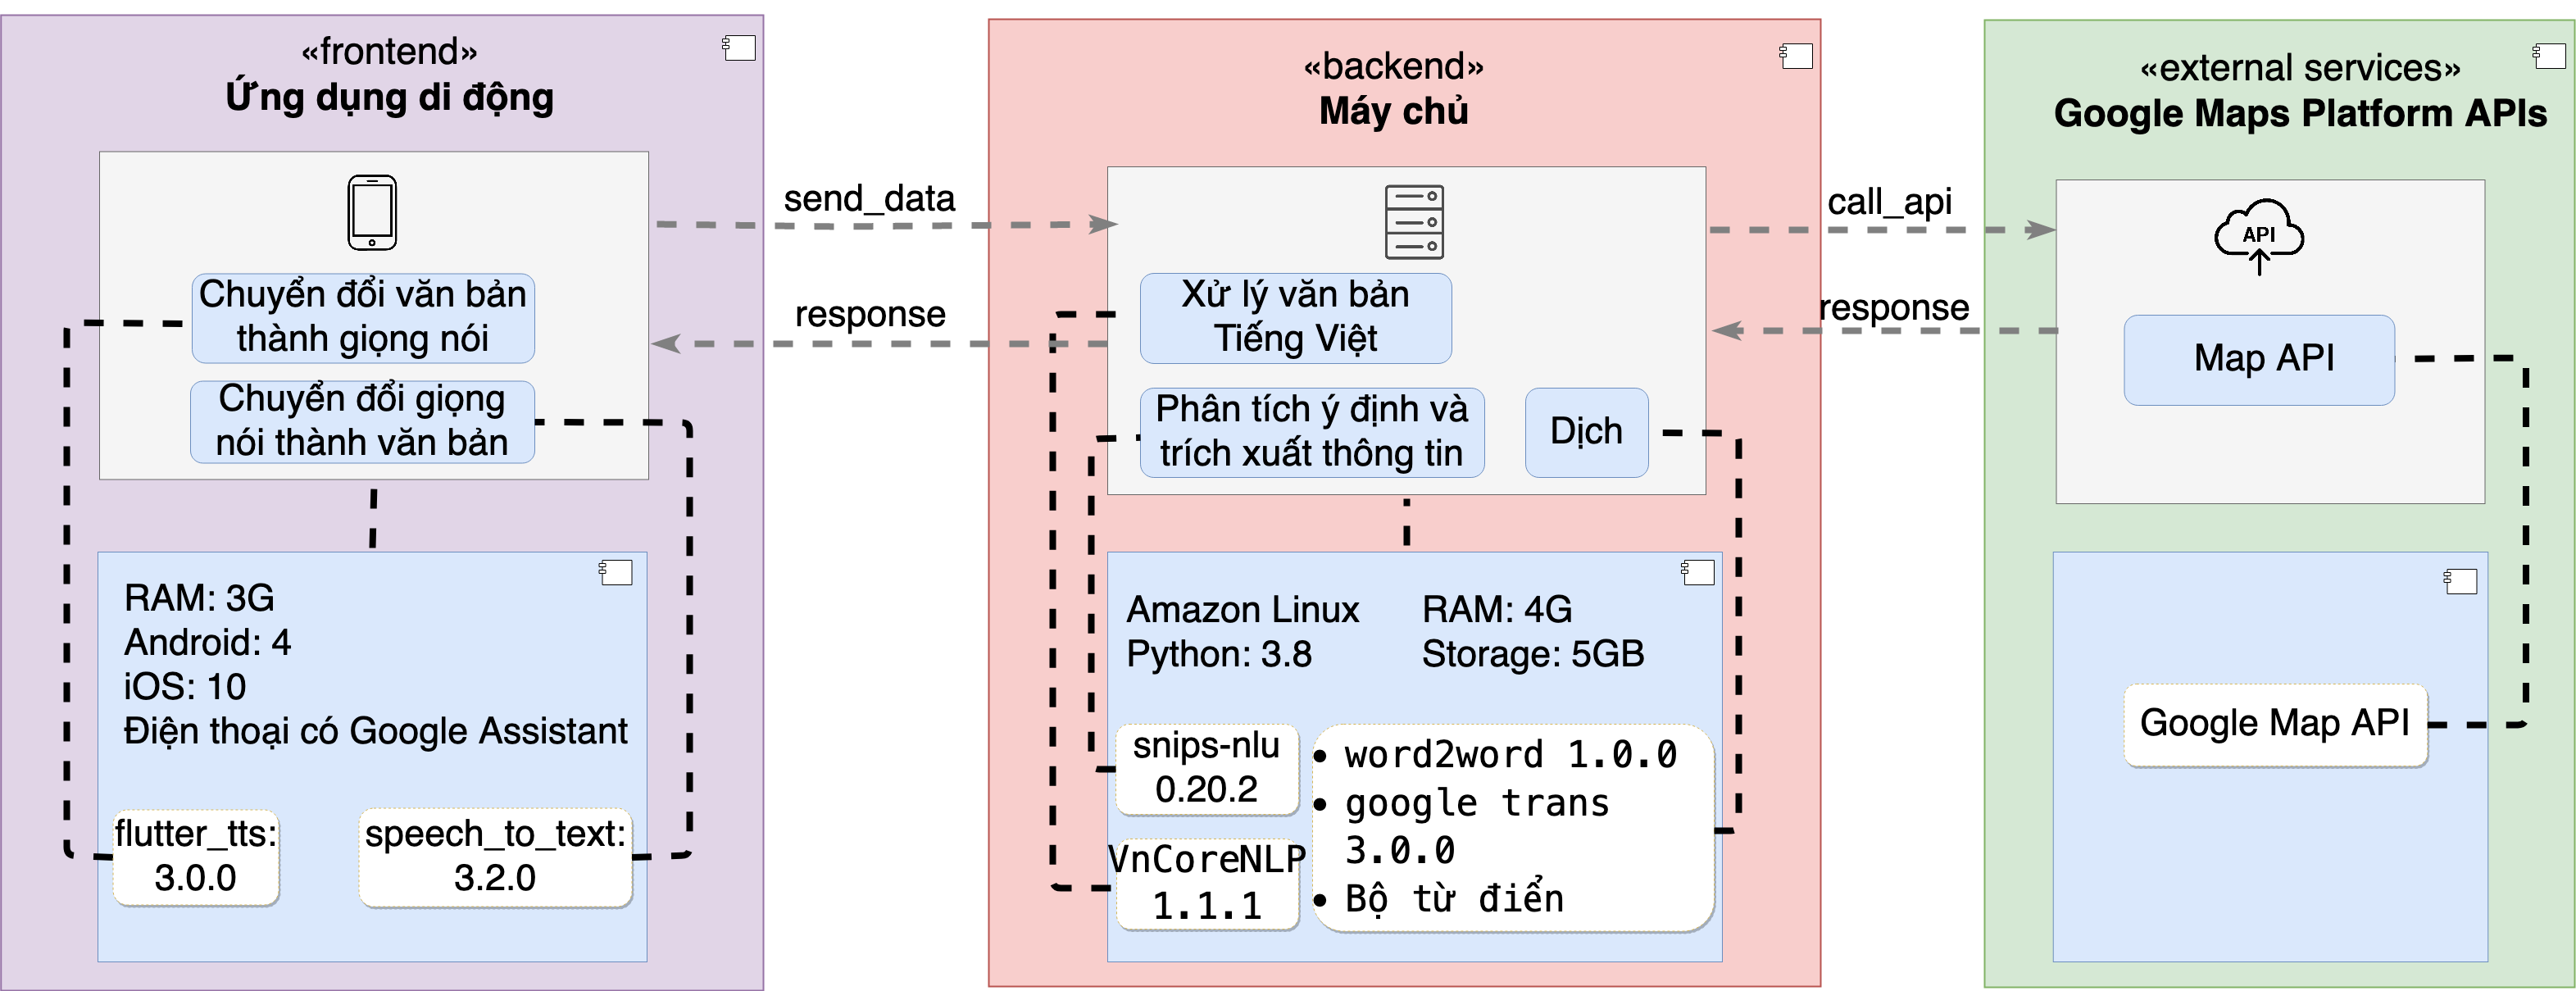
\includegraphics[width=15cm]{images/Structure-System.png}
    \caption{Kiến trúc hệ thống}
    \label{fig:kien-truc-he-thong}
\end{figure}

Máy chủ (Server) thực hiện chương trình xử lý và phân tích dữ liệu. Chương trình này chịu trách nhiệm xử lý dữ liệu gửi lên (Text) bao gồm thành phần: Phân tích ý định (intent), trích xuất dữ liệu và tìm kiếm kết quả trả lời câu hỏi của người gửi. Khi ứng dụng điện thoại gửi Text lên, chương trình xử lý rồi trả về kết quả trên ứng dụng điện thoại. Máy chủ sẽ cung cấp các API tương ứng. Các API cung cấp giao diện cho phép app di động giao tiếp với chương trình xử lý ở máy chủ.

Trong phạm vi đề tài, nhóm sẽ xây dựng thành phần xác định ý định (intent), trích xuất dữ liệu và tìm kiếm kết quả trả lời câu hỏi sẽ sử dụng API của Google Map\cite{google-map}.

Phầm mềm ứng dụng cung cấp một giao diện người dùng qua ứng dụng trên điện thoại di động. Giao diện này cho phép người dùng sử dụng để hỏi các câu hỏi về chỉ đường từ một địa chỉ này đến một địa chỉ khác cụ thể bằng giọng nói (ghi âm câu nói) hoặc là nhập văn bản trên ứng dụng và trả về cho người dùng kết quả phù hợp.
\begin{itemize}
    \item[--] Chuyển giọng nói thành văn bản: Chuyển câu lệnh bằng giọng nói của người dùng thành văn bản để hiển thị lên ứng dụng và gửi lên hệ thống.
    \item[--] Chuyển văn bản thành giọng nói: Chuyển phản hồi của hệ thống thành dạng âm thanh để phát ra qua điện thoại.
\end{itemize}

Hai thành phần chuyển giọng nói thành văn bản và chuyển văn bản thành giọng nói được thực hiện ở ứng dụng di động bằng cách sử dụng package speech\_to\_text\cite{stt} và flutter\_tts\cite{tts} được cung cấp bởi bộ quản lý thư viện của Flutter.

\section{Xây dựng Use Case}
Hình dưới đây thể hiện các chức năng chính của ứng dụng (Xem hình \ref{fig:UC}). 
\begin{figure}[H]
    \centering
    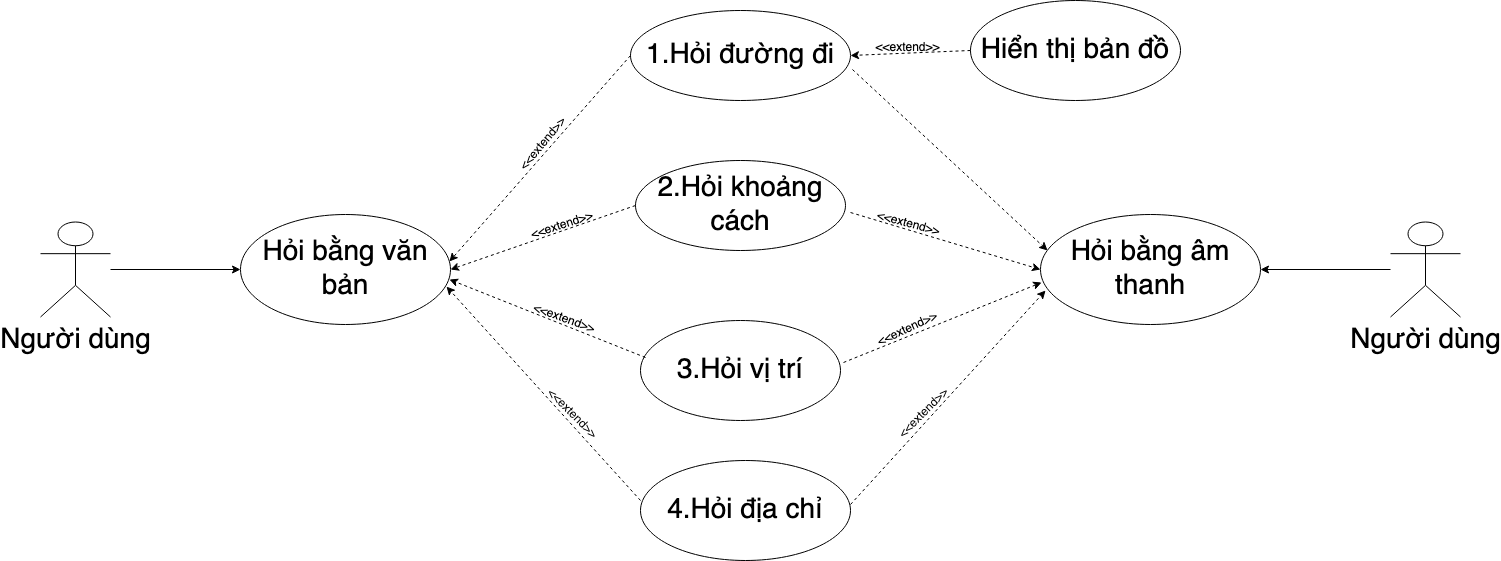
\includegraphics[width=15cm]{images/ChatbotSRS-UseCase.png}
    \caption{Use Diagram}
    \label{fig:UC}
\end{figure}

Các chức năng chính của ứng dụng:
\begin{itemize}
    \item[--] Hỏi bằng giọng nói. 
    \item[--] Hỏi bằng văn bản.
    \item[--] Đường đi từ một địa điểm đến một địa điểm.
    \item[--] Hỏi vị trí hiện tại.
    \item[--] Hỏi địa chỉ chính xác của một địa danh cụ thể.
    \item[--] Hỏi khoảng cách từ một địa điểm đến một địa điểm.
    \item[--] Xem giao diện bản đồ chỉ đường đi. 
\end{itemize}

\section{Xây dựng luồng ứng dụng - Flow Diagram}
Hình dưới đây thể hiện quy trình thực hiện của ứng dụng (Xem hình \ref{fig:Sequence-Diagram}). 
\begin{figure}[H]
    \centering
    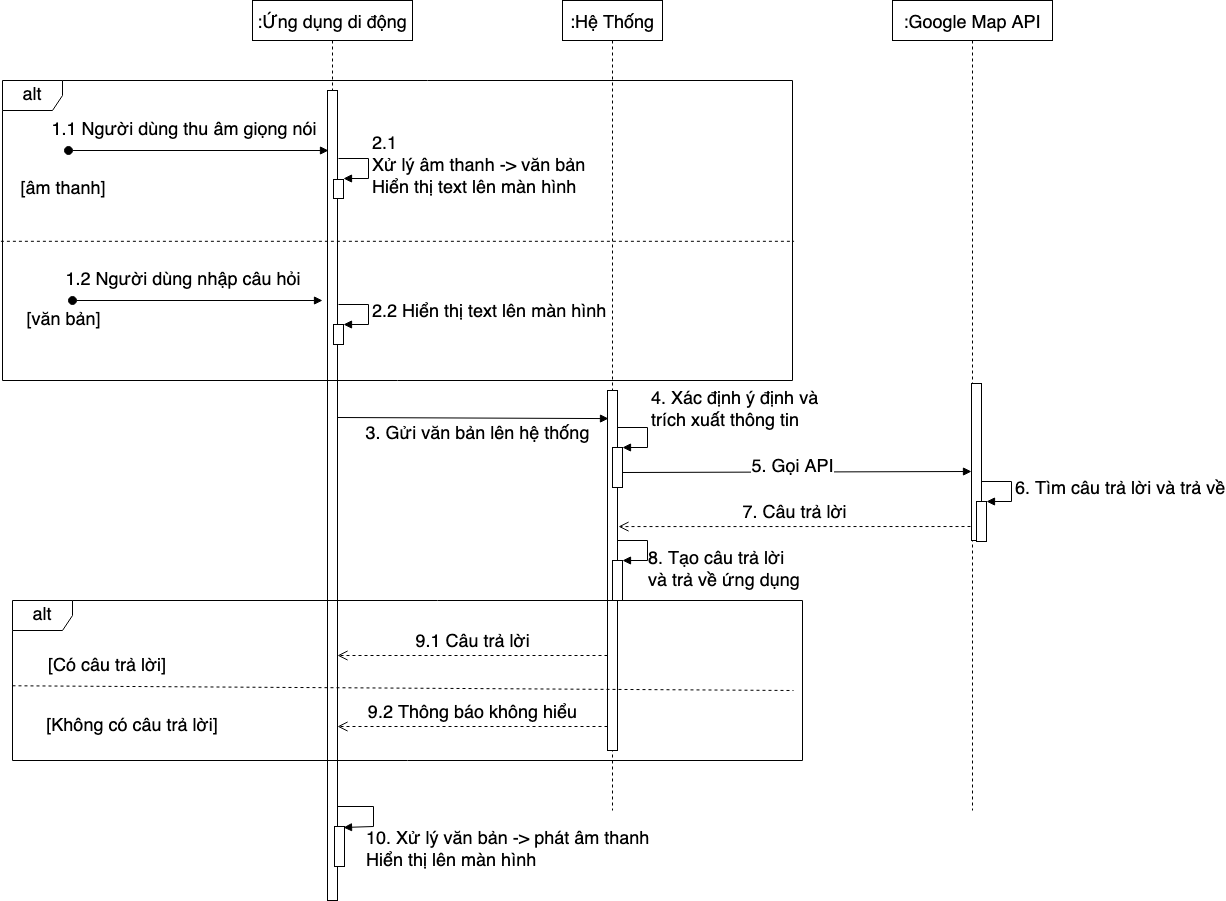
\includegraphics[width=15cm]{images/ChatbotSRS-Sequence.png}
    \caption{Flow Diagram}
    \label{fig:Sequence-Diagram}
\end{figure}
Khi người dùng sử dụng ứng dụng và chọn chức năng trò chuyện, ứng dụng sẽ xuất hiện hộp thoại cuộc trò chuyện. Dưới đây là thiết kế quy trình xử lý dữ liệu và trả về kết quả cho người dùng:
\begin{itemize}
    \item[--] Bước 1: Người dùng gửi dữ liệu cho ứng dụng bằng hai cách:
    \begin{itemize}
        \item[\textbullet] Bước 1.1: Người dùng thực hiện thu âm giọng nói bằng ứng dụng.
        \item[\textbullet] Bước 1.2: Người dùng trực tiếp nhập văn bản trên ứng dụng.
    \end{itemize} 
    \item[--] Bước 2: Nếu người dùng sử dụng giọng nói (1.1), ứng dụng thực hiện chuyển đổi giọng nói thành văn bản. Hiển thị văn bản lên màn hình cuộc hội thoại.
    \item[--] Bước 3: Ứng dụng gửi văn bản lên hệ thống. 
    \item[--] Bước 4: Hệ thống thực hiện xác định ý định (intent) và trích xuất thông tin. 
    \item[--] Bước 5: Dựa vào thông tin vừa phân tích được, tiến hành gọi (call) Google Map API.
    \item[--] Bước 6: GoogleMaps tiến hành tìm kiếm câu trả lời và trả về.
    \item[--] Bước 7: Gửi câu trả lời về hệ thống.
    \item[--] Bước 8: Hệ thống tạo câu trả lời và trả về ứng dụng. 
    \item[--] Bước 9:  
    \begin{itemize}
        \item[\textbullet] Bước 9.1: Câu trả lời được gửi về ứng dụng.
        \item[\textbullet] Bước 9.2: Thông báo không hiểu gửi về ứng dụng.
    \end{itemize} 
    \item[--] Bước 10: Ứng dụng thực hiện chuyển đổi văn bản thành âm thanh. Hiển thị văn bản lên màn hình và phát lên nội dung văn bản đó.
\end{itemize}

\section{Sơ đồ lớp}
\subsection{Sơ đồ lớp Backend}
\begin{figure}[H]
    \centering
    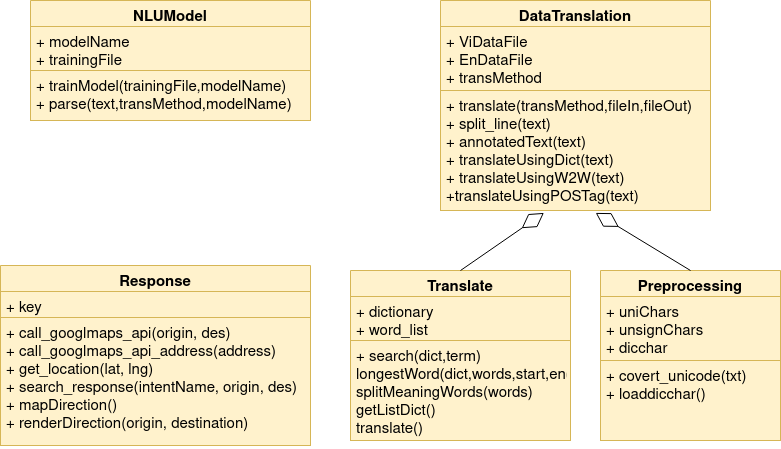
\includegraphics[width=15cm]{images/serverclassdiagram.png}
    \caption{Sơ đồ lớp Backend}
    \label{fig:serverclassdiagram} 
\end{figure}

Hình \ref{fig:serverclassdiagram} thể hiện sơ đồ lớp được xây dựng ở Backend. Các lớp được thể hiện như sau:

\begin{itemize}
    \item[--] NLUModel: Class này gồm các phương thức để xây dựng mô hình phân lớp và dự đoán đầu vào mới.
    \item[--] Preprocesing: Gồm các phương thức cho việc tiền xử lý dữ liệu.
    \item[--] Translate: Xây dựng thuật toán so khớp từ dài nhất (longest matching) áp dụng cho việc dịch bằng từ điển.
    \item[--] DataTranslation: Gồm các phương thức để dịch tập dữ liệu từ tiếng Việt sang tiếng Anh.
    \item[--] Response: Class này dùng để tạo ra câu trả lời với ý định tương ứng.
    
\end{itemize}


\subsection{Sơ đồ lớp Frontend (mobile)}
\begin{figure}[H]
    \centering
    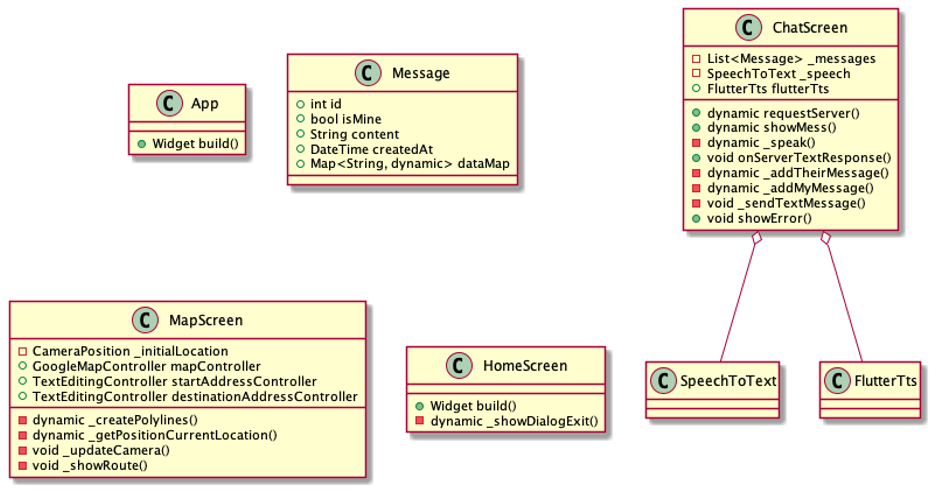
\includegraphics[width=15cm]{images/classdiagram.png}
    \caption{Sơ đồ lớp Frontend}
    \label{fig:classdiagram} 
\end{figure}
Hình \ref{fig:classdiagram} thể hiện sơ đồ lớp được xây dựng ở Frontend. Các lớp được thể hiện như sau:

\begin{itemize}
    \item[--] App: Class chính để xây dựng (build) ứng dụng.
    \item[--] Message: Thể hiện cấu trúc đối tượng Message (tin nhắn) được xây dựng. 
    \item[--] ChatScreen: Xây dựng màn hình chat của ứng dụng.
    \item[--] MapScreen: Xây dựng màn hình bản đồ của ứng dụng.
    \item[--] HomeScreen: Màn hình chọn chức năng "Nói chuyện" và thoát khỏi ứng dụng.
    \item[--] SpeechToText: Class thể hiện thư viện chuyển đổi giọng nói thành văn bản.  
    \item[--] TTSpeech: Class thể hiện thư viện chuyển đổi văn bản thành giọng nói.  
\end{itemize}


\section{Xây dựng thành phần xác định ý định và trích xuất thực thể}
\subsection{Tạo dữ liệu tiếng Việt}
Nhóm đã thực hiện tạo dữ liệu gồm 4 ý định (intent) thuộc lĩnh vực đường đi:

\begin{itemize}
    \item[--] Đường đi từ một địa điểm đến một địa điểm - "findRouteAB"
    \item[--] Hỏi vị trí hiện tại - "askLocation"
    \item[--] Hỏi địa chỉ chính xác của một địa danh cụ thể - "askAddress"
    \item[--] Hỏi khoảng cách từ một địa điểm đến một địa điểm - "askDistance"
\end{itemize}

Bộ dữ liệu huấn luyện tiếng Việt gồm 3200 câu mẫu, mỗi ý định 800 câu mẫu. Dữ liệu huấn luyện được tạo với sự hỗ trợ của công cụ Chatito\footnote{Công cụ Chatito \url{https://github.com/rodrigopivi/Chatito}}.

Bộ dữ liệu kiểm thử tiếng Việt khoảng 120 câu mẫu. Mỗi ý định khoảng 30 câu. Các câu mẫu này được thu thập từ người dùng thật. Để tiến hành tạo dữ liệu kiểm thử bằng tiếng Việt, chúng em thực hiện như sau:

\begin{itemize}
    \item[--] Bước 1: Tạo dữ liệu trên file txt\footnote{Dữ liệu huấn luyện tiếng Việt \url{https://drive.google.com/drive/folders/1A21k70s_pb2vQf8jFDm2ueuNehWyBwPU?usp=sharing}}. 
    \\Ví dụ: Với ý định "Hỏi đường đi (findRouteAB)" ta có: "Đường đi từ đại học Sài Gòn đến Cao đẳng Sài Gòn"
    \item[--] Bước 2: Viết một chương trình nhỏ để tiến hành chuyển dữ liệu từ file txt sang dạng json để thuận tiện cho việc huấn luyện (Xem hình dữ liệu dưới dạng file json Hình \ref{fig:data-train-json} ). Dữ liệu tiếng Việt đầy đủ có thể xem tại đây \footnote{Dữ liệu huấn luyện tiếng Việt \url{https://drive.google.com/file/d/1tRmJwKgtK5jKoiN57r7oAukfUO-UN4Ip/view?usp=sharing}}\footnote{Dữ liệu kiểm thử tiếng Việt \url{https://drive.google.com/file/d/1LUvQ7sz2JcdRYUkGVOgJBqqo10O6hhkP/view?usp=sharing}}
\end{itemize}
Hình ảnh dưới đây minh hoạ một câu dữ liệu dưới dang json trước khi tiến hành dịch (Xem hình \ref{fig:data-train-json})
\begin{figure}[H]
    \centering
    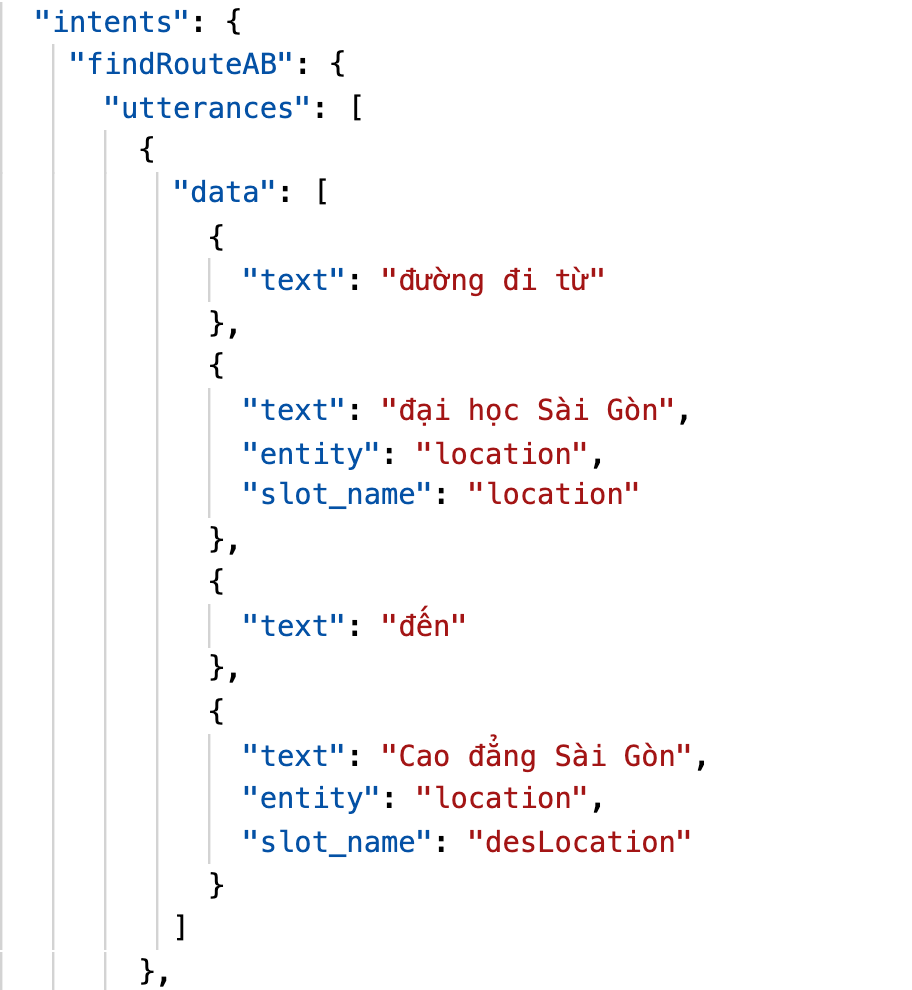
\includegraphics[width=10cm]{images/Data-train-json.png}
    \caption{Hình ảnh minh họa dữ liệu trước khi dịch}
    \label{fig:data-train-json}
\end{figure}
\subsection{Huấn luyện dữ liệu}
Chúng em đã tiến hành tạo bộ dữ liệu dùng để huấn luyện dưới đây để thực hiện chuyển hoá ngôn ngữ từ tiếng Việt sang tiếng Anh.
\begin{itemize}
    \item[--] Tập train: 3200 câu bao gồm mỗi loại 800 câu\footnote{Xem thêm về bộ huấn luyện \url{https://drive.google.com/file/d/1VSDhjrSghKtHmQxhWfC_x-qyOKDm3YuM/view?usp=sharing}}.
    \item[--] Tập test: 120 câu bao gồm mỗi loại khoảng 30 câu\footnote{Xem thêm về bộ kiểm thử \url{https://drive.google.com/file/d/1S631oRroP67z6LRwGSNwkrx-22c10baJ/view?usp=sharing}}.
\end{itemize}

Thông qua kết quả của quá trình thực hiện chuyển hoá dữ liệu từ tiếng Việt sang tiếng Anh để chuẩn bị dữ liệu cho quá trình huấn luyện mà chúng em đã tiến hành nghiên cứu, chúng em nhận thấy kết quả của việc "Xây dựng bộ từ điển" cho riêng ứng dụng theo các chủ đề, lĩnh vực cụ thể đem lại hiệu quả tốt trong quá trình dịch và không làm sai lệnh ngữ nghĩa của câu. Vì vậy chúng em chọn giải pháp "Xây dựng bộ từ điển" để thực hiện chuyển hoá dữ liệu sang tiếng Anh để tiến hành thực hiện huấn luyện dữ liệu. Hình \ref{fig:dictonary} là hình ảnh minh họa của bộ từ điển mà nhóm em sử dụng. Hình \ref{fig:data-train-en} hiển thị dữ liệu tiếng Anh dưới dạng json để thực hiện tiến hành huấn luyện dữ liệu. Kết quả của việc tạo bộ dữ liệu tiếng Anh tự động được lưu trữ tại đây\footnote{Dữ liệu huấn luyện tiếng Anh \url{https://drive.google.com/file/d/1VSDhjrSghKtHmQxhWfC_x-qyOKDm3YuM/view?usp=sharing}}\footnote{Dữ liệu kiểm thử tiếng Anh \url{https://drive.google.com/file/d/1S631oRroP67z6LRwGSNwkrx-22c10baJ/view?usp=sharing}}.

\begin{figure}[H]
    \centering
    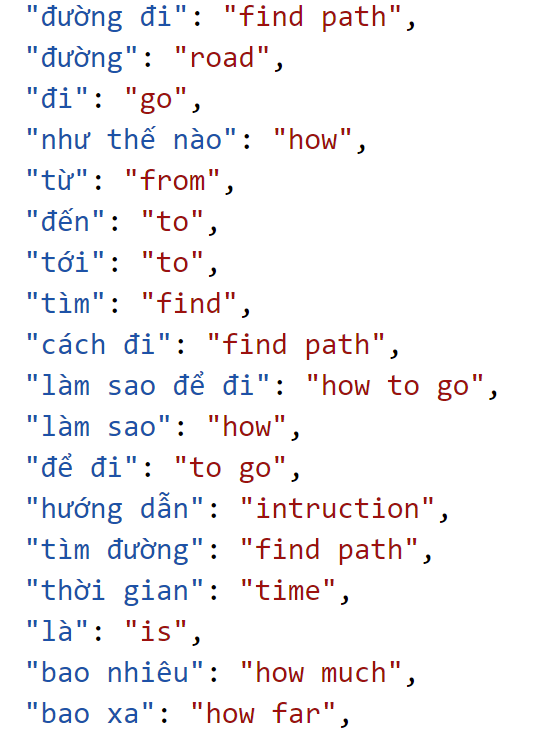
\includegraphics[width=10cm]{images/dictionary.png}
    \caption{Hình ảnh minh họa của từ điển}
    \label{fig:dictonary} 
\end{figure}



\begin{figure}[H]
    \centering
    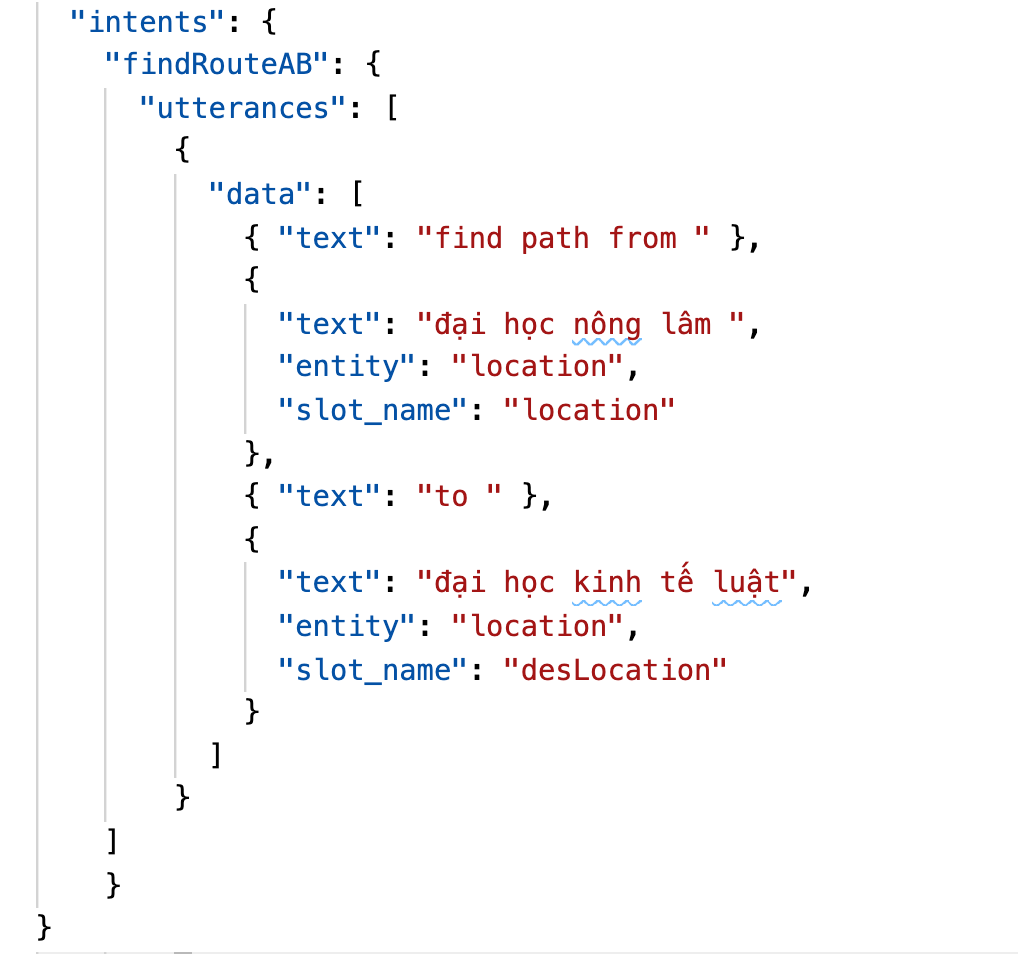
\includegraphics[width=15cm]{images/Data-train-ex.png}
    \caption{Hình ảnh minh họa dữ liệu sau khi dịch}
    \label{fig:data-train-en} 
\end{figure}


Bài toán phân lớp (Classification) là quá trình phân lớp một đối tượng dữ liệu vào một hay nhiều lớp đã cho trước nhờ một mô hình phân lớp (model). Mô hình này được xây dựng dựa trên một tập dữ liệu được xây dựng trước đó có gán nhãn (hay còn gọi là tập huấn luyện). Quá trình phân lớp là quá trình gán nhãn cho đối tượng dữ liệu.



Để xây dựng mô hình phân lớp ý định và trích xuất các thực thể, nhóm em thực hiện các bước như hình \ref{fig:FlowTrainingData}:

\begin{figure}[H]
    \centering
    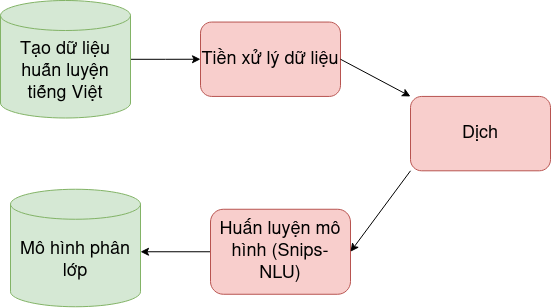
\includegraphics[width=15cm]{images/FlowTrainingData.png}
    \caption{Các bước huấn luyện mô hình phân lớp}
    \label{fig:FlowTrainingData}
\end{figure}

\begin{itemize}

    \item[--]Tạo dữ liệu tiếng Việt: dữ liệu được tạo với các câu nói ngôn ngữ tiếng Việt được dùng trong lĩnh vực hỏi đường, các câu nói này thuộc 4 mục đích khác nhau bao gồm: hỏi vị trí hiện tại của bản thân, hỏi địa chỉ của một địa điểm nào đó, hỏi khoảng cách giữa 2 địa điểm và hỏi cách đi giữa 2 điểm A và B. Các câu nói này đều được gán nhãn với ý định (intent) tương ứng. Các thực thể (entity) như "địa điểm" cũng được "đánh dấu" để cho mô hình có thể học. Dữ liệu sẽ được lưu trong file json. Dữ liệu tiếng Việt đầy đủ có thể xem tại đây \footnote{Dữ liệu huấn luyện tiếng Việt \url{https://drive.google.com/file/d/1tRmJwKgtK5jKoiN57r7oAukfUO-UN4Ip/view?usp=sharing}}
    \footnote{Dữ liệu kiểm thử tiếng Việt \url{https://drive.google.com/file/d/1LUvQ7sz2JcdRYUkGVOgJBqqo10O6hhkP/view?usp=sharing}}.

\item[--]Tiền xử lý dữ liệu: bao gồm chuẩn hóa Unicode tiếng Việt, chuẩn hóa kiểu gõ dấu, đưa về dạng viết thường, xóa bỏ các ký tự không cần thiết.

\item[--]Dịch: áp dụng chuyển hóa dữ liệu từ tiếng Việt sang tiếng Anh bằng phương pháp "Xây dựng bộ từ điển". Kết quả thu được là bộ dữ liệu huấn luyện bằng tiếng Anh lưu ở định dạng file json. Bộ dữ liệu tiếng Anh đầy đủ có thể xem tại đây \footnote{Dữ liệu huấn luyện tiếng Anh \url{https://drive.google.com/file/d/1VSDhjrSghKtHmQxhWfC_x-qyOKDm3YuM/view?usp=sharing}}
    \footnote{Dữ liệu kiểm thử tiếng Anh \url{https://drive.google.com/file/d/1S631oRroP67z6LRwGSNwkrx-22c10baJ/view?usp=sharing}}.

\item[--]Huấn luyện mô hình: dữ liệu huấn luyện tiếng Anh đưa vào mô hình để học tập và trích xuất ra các luật, từ đó tạo ra mô hình phân lớp.
\item[--]Mô hình phân lớp: được sử dụng để trích xuất ý định (intent) và cách thực thể (intent) từ những câu nói mới.
\end{itemize}





\chapter{Kết quả}
\label{Chapter6}

\emph{Chương này trình bày kết quả đề tài, kết quả phát hiện intent, trích xuất thông tin và các chức năng đã cài đặt được.}

\section{Kết quả huấn luyện dữ liệu}

Có rất nhiều cách đánh giá một mô hình phân lớp. Tuỳ vào những bài toán khác nhau mà chúng ta sử dụng các phương pháp khác nhau. Các phương pháp thường được sử dụng là: accuracy score, confusion matrix, ROC curve, Area Under the Curve, Precision and Recall, F1 score, Top R error,... Chúng em sử dụng đánh giá F1 Score để đánh giá phân lớp các mô hình. Sau đây là khái quát một số khái niệm để chúng ta hiểu rõ hơn về kết quả đánh giá.

\begin{itemize}
    \item[--] Accuracy là tỉ lệ giữa số điểm được phân loại đúng và tổng số điểm trong dữ liệu kiểm thử. Accuracy chỉ phù hợp với các bài toán mà kích thước các lớp dữ liệu là tương đối như nhau.
    \item[--] Confusion matrix giúp có cái nhìn rõ hơn về việc các điểm dữ liệu được phân loại đúng/sai như thế nào.
    \item[--] True Positive (TP): số lượng điểm của lớp positive được phân loại đúng là positive.
    \item[--] True Negative (TN): số lượng điểm của lớp negative được phân loại đúng là negative.
    \item[--] False Positive (FP): số lượng điểm của lớp negative bị phân loại nhầm thành positive.
    \item[--] False Negative (FN): số lượng điểm của lớp positive bị phân loại nhầm thành negative
\end{itemize}

Precision được định nghĩa là tỉ lệ số điểm true positive trong số những điểm được phân loại là positive (TP + FP).
\begin{center}
    Precision = $\dfrac{TP}{TP+EP}$
\end{center}

Recall được định nghĩa là tỉ lệ số điểm true positive trong số những điểm thực sự là positive (TP + FN).
\begin{center}
    Recall = $\dfrac{TP}{TP+FN}$
\end{center}

$F_{1}$-score có giá trị nằm trong nửa khoảng (0,1]. F1 càng cao, bộ phân lớp càng tốt. Khi cả recall và precision đều bằng 1 (tốt nhất có thể), F1=1
\begin{center}
    $F_{1}=2\frac{1}{\frac{1}{\text{Precision}} + \frac{1}{\text{recall}}}= 2\frac{\text{precision} \times \text{recall}}{\text{precision} + \text{recall}}$
\end{center}

Chúng em xây dựng mô hình phân loại các câu hỏi chỉ đường. Nhãn dán của của các quan sát sẽ bao gồm: câu hỏi chỉ đường (findRouteAB), câu hỏi khoảng cách (askDistance), câu hỏi vị trí hiện tại (askLocation), câu hỏi địa chỉ của một địa danh (askAddress). Kích thước của tập dữ liệu như sau:
\begin{itemize}
    \item[--] Tập train: 80 câu bao gồm mỗi loại 20 câu.
    \item[--] Tập test: 40 câu bao gồm mỗi loại 10 câu.
\end{itemize}

Sau khi lựa chọn các loại intent để thực hiện và đã tạo dự liệu để huấn luyện và tiến hành kiểm thử cho từng intent.

Đem bộ dữ liệu để huấn luyện và đánh giá, ta đạt được Confusion matrix như hình \ref{fig:metrics-dict-end}:


\begin{table}[]
    \begin{tabular}{|l|l|llllll}
    \hline
    \textbf{Intent Name} & \multicolumn{3}{l|}{\textbf{Intent Classification}}                                          & \multicolumn{4}{l|}{\textbf{Slot Filling}}                                                                                                                                                                                                                                                         \\ \hline
    \textbf{}            & \textbf{Precision} & \multicolumn{1}{l|}{\textbf{Recall}} & \multicolumn{1}{l|}{\textbf{F1}} & \multicolumn{1}{l|}{\textbf{Slot}}                                                  & \multicolumn{1}{l|}{\textbf{Precision}}                            & \multicolumn{1}{l|}{\textbf{Recall}}                               & \multicolumn{1}{l|}{\textbf{F1}}                                   \\ \hline
    askAddress           & 0.769              & \multicolumn{1}{l|}{1}               & \multicolumn{1}{l|}{0.870}       & \multicolumn{1}{l|}{location}                                                       & \multicolumn{1}{l|}{1}                                             & \multicolumn{1}{l|}{1}                                             & \multicolumn{1}{l|}{1}                                             \\ \hline
    askDistance          & 1                  & \multicolumn{1}{l|}{1}               & \multicolumn{1}{l|}{1}           & \multicolumn{1}{l|}{\begin{tabular}[c]{@{}l@{}}location\\ desLocation\end{tabular}} & \multicolumn{1}{l|}{\begin{tabular}[c]{@{}l@{}}1\\ 1\end{tabular}} & \multicolumn{1}{l|}{\begin{tabular}[c]{@{}l@{}}1\\ 1\end{tabular}} & \multicolumn{1}{l|}{\begin{tabular}[c]{@{}l@{}}1\\ 1\end{tabular}} \\ \hline
    askLocation          & 1                  & \multicolumn{1}{l|}{0.7}             & \multicolumn{1}{l|}{0.824}       & \multicolumn{1}{l|}{}                                                               & \multicolumn{1}{l|}{}                                              & \multicolumn{1}{l|}{}                                              & \multicolumn{1}{l|}{}                                              \\ \hline
    findRouteAB          & 1                  & \multicolumn{1}{l|}{1}               & \multicolumn{1}{l|}{1}           & \multicolumn{1}{l|}{\begin{tabular}[c]{@{}l@{}}location\\ desLocation\end{tabular}} & \multicolumn{1}{l|}{\begin{tabular}[c]{@{}l@{}}1\\ 1\end{tabular}} & \multicolumn{1}{l|}{\begin{tabular}[c]{@{}l@{}}1\\ 1\end{tabular}} & \multicolumn{1}{l|}{\begin{tabular}[c]{@{}l@{}}1\\ 1\end{tabular}} \\ \hline
    Average metrics      & 0.942              & \multicolumn{1}{l|}{0.925}           & \multicolumn{1}{l|}{0.923}       & \multicolumn{1}{l|}{}                                                               & \multicolumn{1}{l|}{1}                                             & \multicolumn{1}{l|}{1}                                             & \multicolumn{1}{l|}{1}                                             \\ \hline
    Accuracy             & 0.925              &                                      &                                  &                                                                                     &                                                                    &                                                                    &                                                                    \\ \cline{1-2}
    \end{tabular}
     \caption{Các chỉ số của mô hình}
        \label{fig:metrics-dict-end}
\end{table}

Các chỉ số được tính cho từng lớp riêng lẻ, ngoại trừ accuracy (độ chính xác); nó được tính toán trên tất cả các lớp để cung cấp độ chính xác phân loại cho mô hình này.

Đánh giá tổng quan: Accuracy (Độ chính xác của toàn bộ dữ liệu) là 0.925.

Đánh giá chi tiết từng phân loại: Dựa trên kết quả F1-Score cho từng phân loại, dễ dàng nhìn thấy độ chính xác của từng loại sẽ được sắp xếp theo thứ tự sau đây: findRouteAB, askDistance ,askLocation, askAddress.

Như vậy, dựa trên kết quả kiểm thử cho thấy độ chính xác khi phát hiện các intent và slot là cao, điều này giúp cho việc phân loại câu hỏi chính xác giúp ứng dụng có thể đưa ra những câu trả lời phù hợp với từng nhu cầu của người dùng.

Dưới đây là kết quả ví dụ với intput: "Đường đi từ Đại học Nông lâm Thành phố Hồ Chí Minh đến Đại học Kinh tế Luật" (xem hình \ref{fig:detect-intent}).

\begin{figure}[htp]
    \centering
    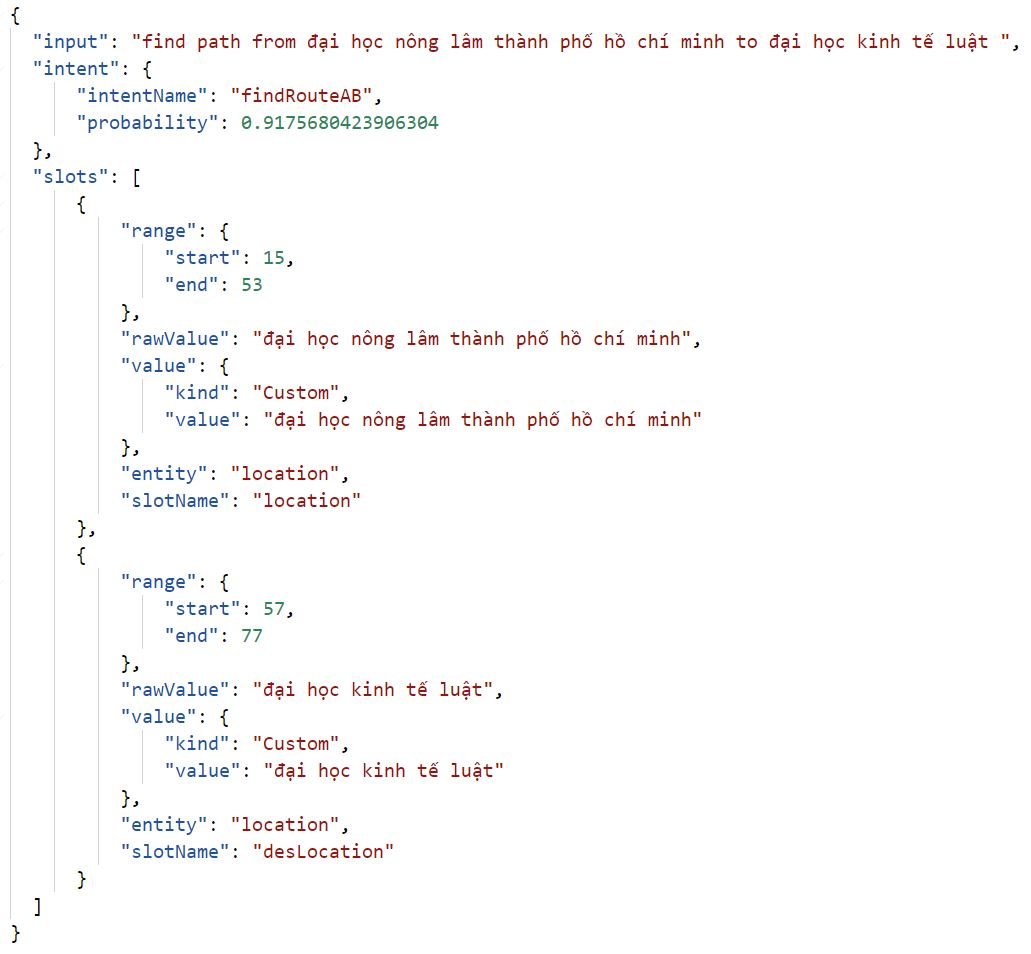
\includegraphics[width=15cm]{images/detect_intent.jpg}
    \caption{Các chỉ số của mô hình}
    \label{fig:detect-intent}
\end{figure}

Với input như trên, hệ thống sẽ chuyển hoá từ ngữ từ tiếng Việt sang tiếng Anh (ngoại trừ các địa danh), sau đó hệ thống sẽ tiến hành phân tích intent và trích xuất slot thu được kết quả như hình \ref{fig:detect-intent}.
\begin{itemize}
    \item[--] Phân loại intent: "findRouteAB"
    \item[--] Địa điểm bắt đầu: "Đại học Nông lâm Thành phố Hồ Chí Minh"
    \item[--] Địa điểm kết thúc: "Đại học Kinh tế Luật"
\end{itemize}

\section{Ứng dụng}
\subsection{Sản phẩm}
Hiện tại, ứng dụng đã được phát triển trên hai nền tảng Android và iOS và đã được đăng tải lên các cửa hàng trên iOS (App Store) (Xem hình \ref{fig:app-store}) và Android (Google Play) (Xem hình \ref{fig:google-play}). Xem và tải ứng dụng trên Android tại đây \footnote{Xem thêm về ứng dụng trên Andoird tại đây:\url{https://bitly.com.vn/5a5xax}} và trên iOS tại đây \footnote{Xem thêm về ứng dụng trên iOS tại đây:\url{https://bitly.com.vn/7gcxli}}

\begin{figure}[H]
    \centering
    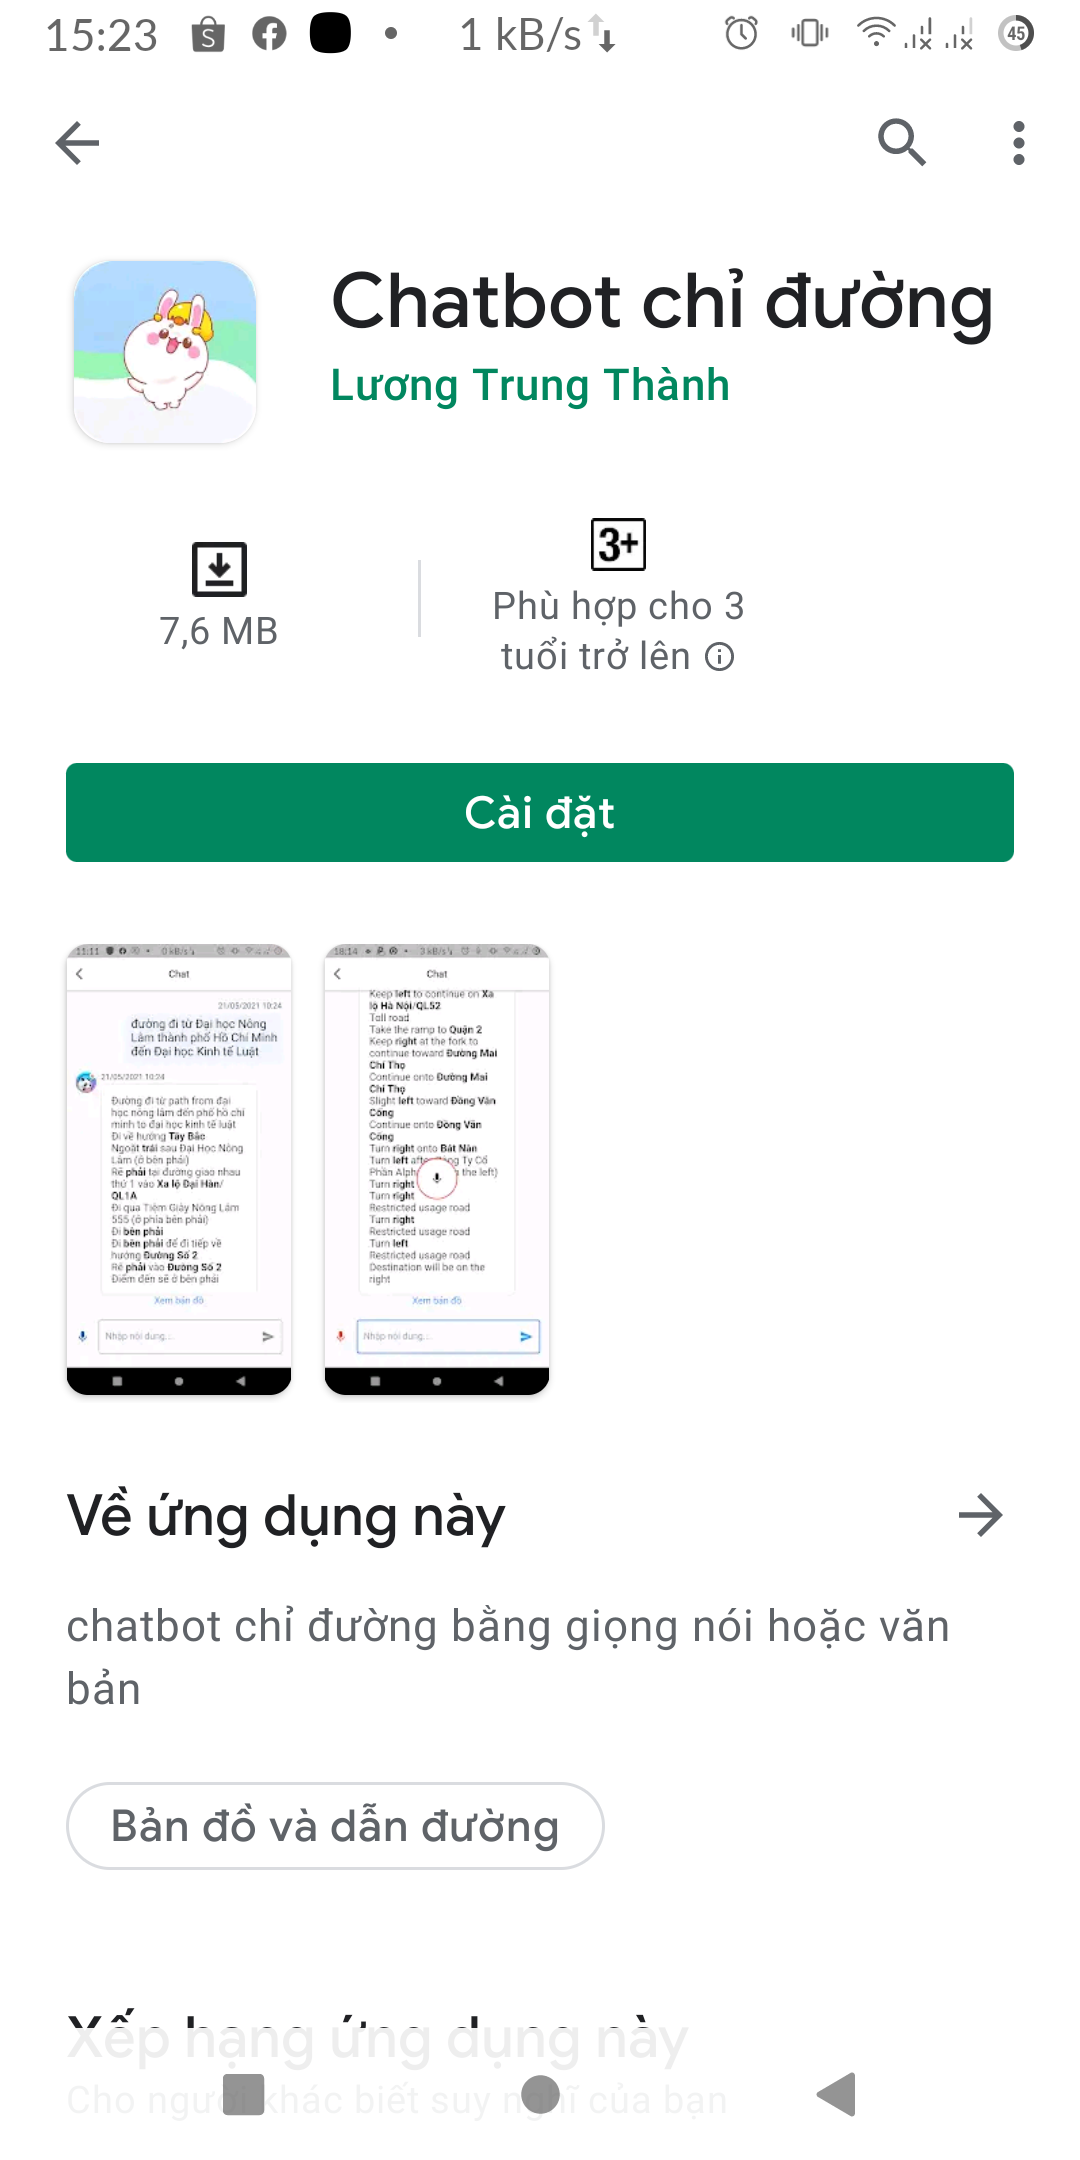
\includegraphics[width=5cm]{images/GooglePlay.jpg}
    \caption{Ứng dụng trên cửa hàng Google Play của Android}
    \label{fig:google-play}
\end{figure}

\begin{figure}[H]
    \centering
    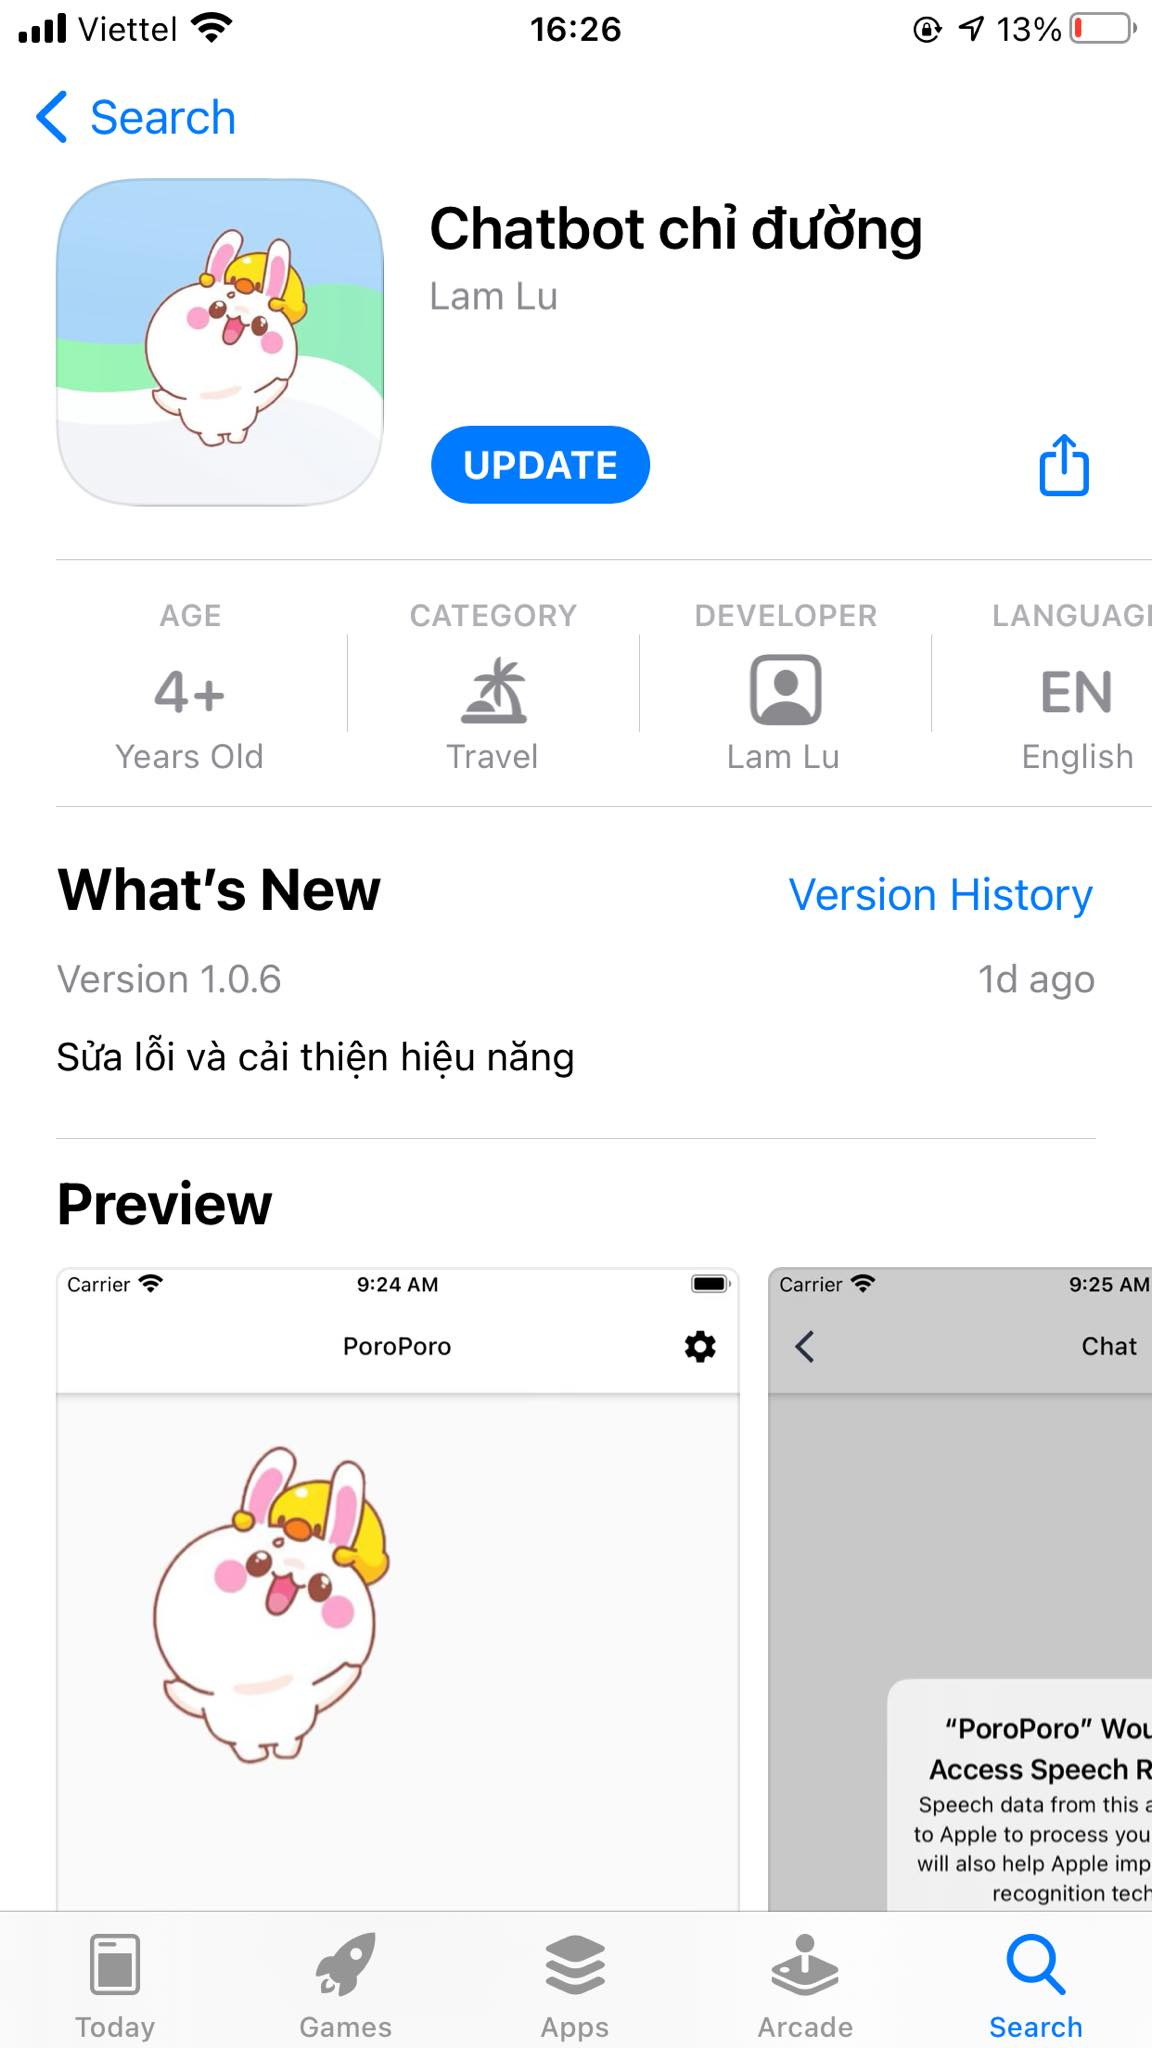
\includegraphics[width=5cm]{images/AppStore.jpg}
    \caption{Ứng dụng trên cửa hàng App Store của iOS}
    \label{fig:app-store}
\end{figure}

\subsection{Các chức năng chính của ứng dụng}

Ứng dụng chatbot được sử dụng với ngôn ngữ chính là tiếng Viêt, dữ liệu đầu vào và đầu ra bao gồm giọng nói và văn bản được xây dựng trong lĩnh vực hỏi đường đi trong phạm vi Thành phố Thủ Đức.
\begin{itemize}
    \item[--] Hỏi đường bằng văn bản: Người dùng nhập 1 câu hỏi bằng văn bản vào ứng dụng. VD: “Đường đi từ UBND thành phố Thủ Đức đến Công An thành phố Thủ Đức”. Bấm nút gửi
    \item[--] Hỏi đường bằng giọng nói: Người dùng nhấn icon ghi âm và nói một câu vào ứng dụng. VD: “Đường đi từ UBND thành phố Thủ Đức đến Công An thành phố Thủ Đức”
    \item[--] Ứng dụng hiển thị câu trả lời bằng văn bản lên màn hình và chuyển văn bản thành âm thanh phát lên.
    \item[--] Ở màn hình bản đồ, bạn có thể xem được đường đi cụ thể mà bạn vừa yêu cầu và khoảng cách sẽ được hiển thị lên bản đồ. Bạn có thể phóng to, thu nhỏ bản đồ và có thể xem vị trí hiện tại của mình.
\end{itemize}
\textbf{Ứng dụng được xây dựng dựa trên các ý định:}
\begin{itemize}
    \item[--] Hỏi đường đi từ một địa điểm đến một địa điểm
    \item[--] Hỏi khoảng cách từ một địa điểm đến một địa điểm
    \item[--] Hỏi vị trí hiện tại của người dùng
    \item[--] Hỏi địa chỉ của một địa điểm  
\end{itemize}
\textbf{Giao diện chức năng hội thoại:}

Giao diện ứng dụng khi mở lên sẽ hiển thị như sau (hình \ref{fig:home}):
\begin{figure}[H]
    \centering
    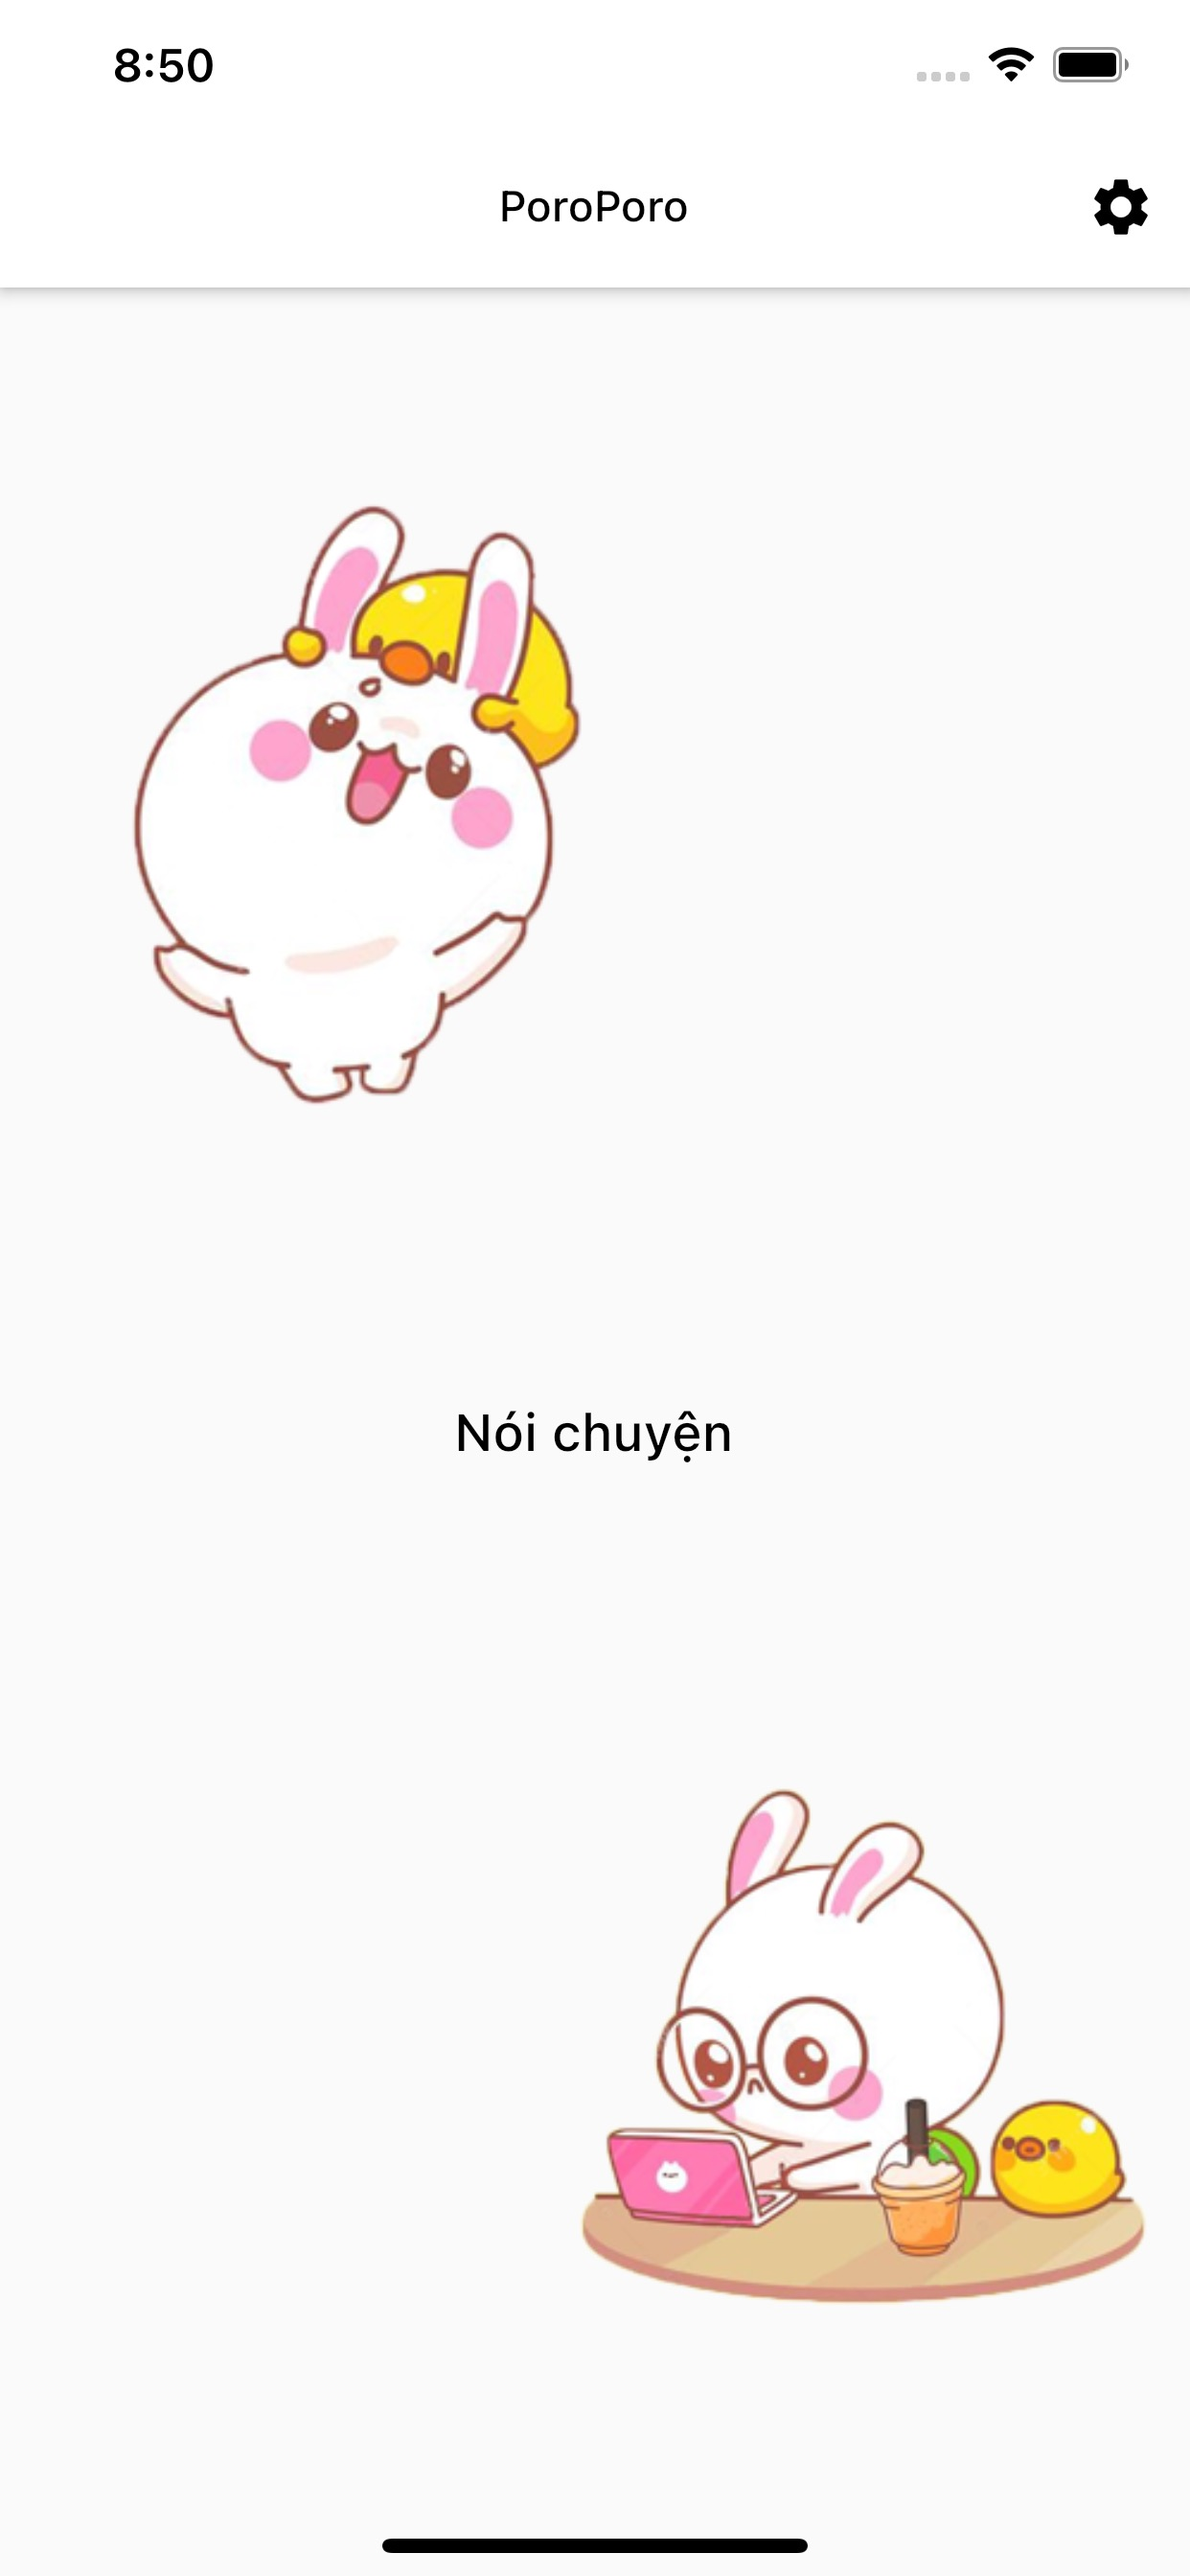
\includegraphics[width=5cm]{images/home.jpg}
    \caption{Màn hình trò chuyện}
    \label{fig:home}
\end{figure}
Khi nhấn vào button "Nói chuyện", màn hình sẽ chuyển sang màn hình cuộc hội thoại.
Giao diện ứng dụng khi thực hiện các đoạn hội thoại giữa người và máy sẽ hiển thị như sau (hình \ref{fig:screen-chat}) :
\begin{figure}[H]
    \centering
    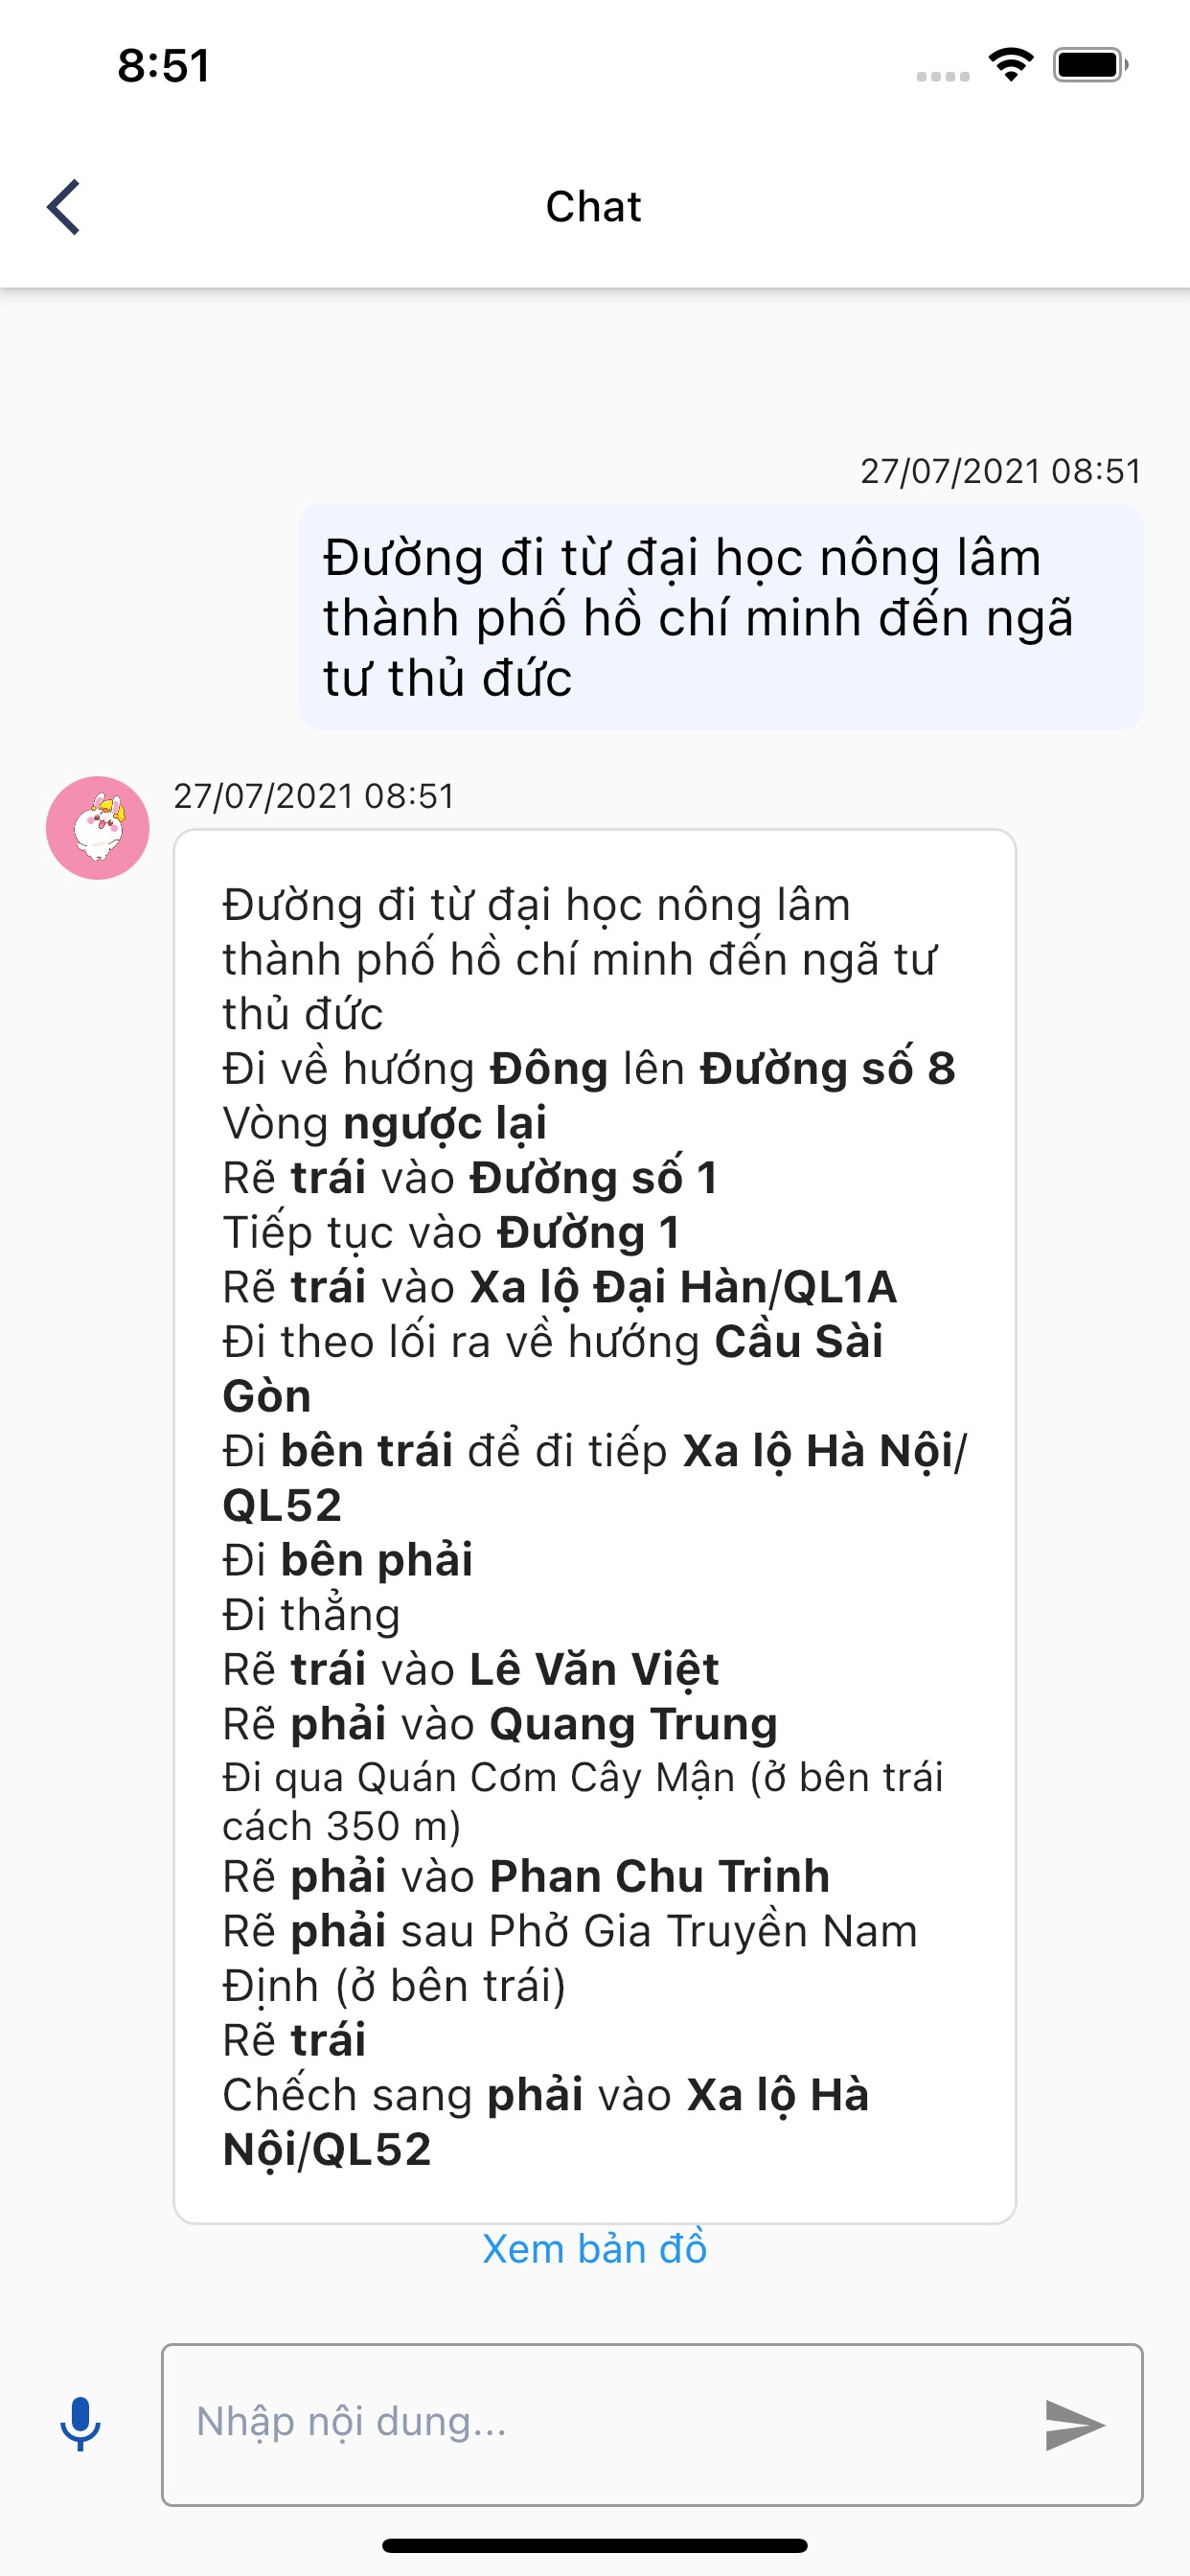
\includegraphics[width=5cm]{images/Screen-chat.jpg}
    \caption{Màn hình trò chuyện}
    \label{fig:screen-chat}
\end{figure}

Giao diện gồm các phần sau đây:
\begin{itemize}
    \item[--] Thanh nhập dữ liệu để người dùng nhập văn bản, một nút ghi âm dùng để ghi âm giọng nói, một nút bấm để thực hiện gửi yêu cầu từ người dùng đến hệ thống.
    \item[--] Bên phải khung hình hiển thị dữ liệu người dùng nhập vào.
    \item[--] Bên trái khung hình hiển thị trả lời từ ứng dụng.
    \item[--] Thời gian tin nhắn được gửi đi và thời gian nhận được phản hồi.
    \item[--] Khi tìm kiếm kết quả thành công, kết quả hướng dẫn đường đi được trả về, button "Xem đường đi" dùng để chuyển sang màn hình bản đồ chỉ đường.
\end{itemize}

Khi người dùng bấm vào icon "micro" trên màn hình cuộc hội thoại, nếu đây là lần đầu sử dụng ứng dụng với chức năng này, ứng dụng sẽ xin người dùng cấp quyền cho phép ghi âm từ thiết bị (xem hình \ref{fig: accesss-mic}), khi chọn cho phép, người dùng có thể sử dụng chức năng này để ghi âm giọng nói.

\begin{figure}[H]
    \centering
    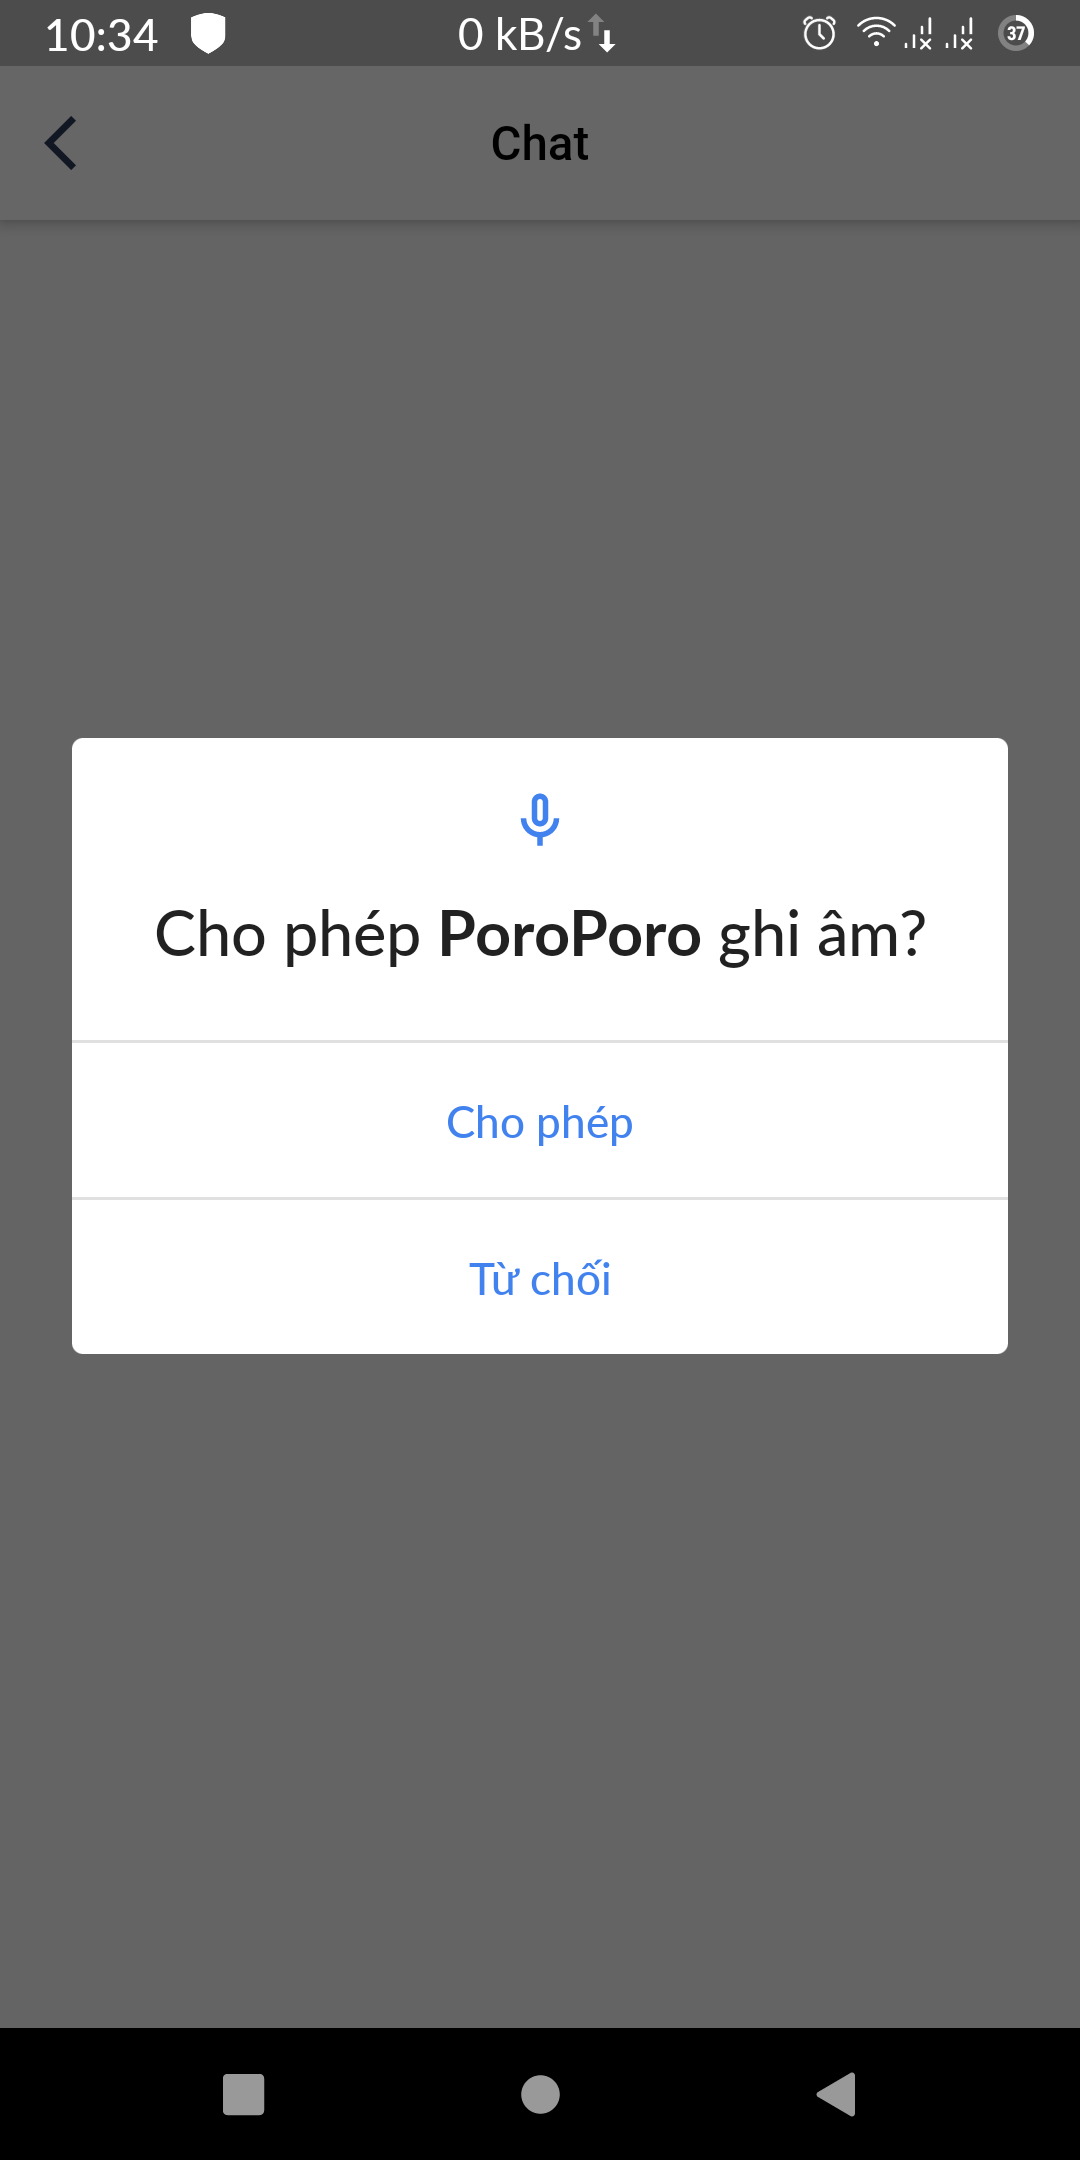
\includegraphics[width=5cm]{images/access_mic.jpg}
    \caption{Màn hình xin quyền cấp phép ghi âm của thiết bị}
    \label{fig: accesss-mic}
\end{figure}

Giao diện ứng dụng khi đang thực hiện ghi âm giọng nói sẽ hiển thị như sau (hình \ref{fig:screen-record}) :

\begin{figure}[H]
    \centering
    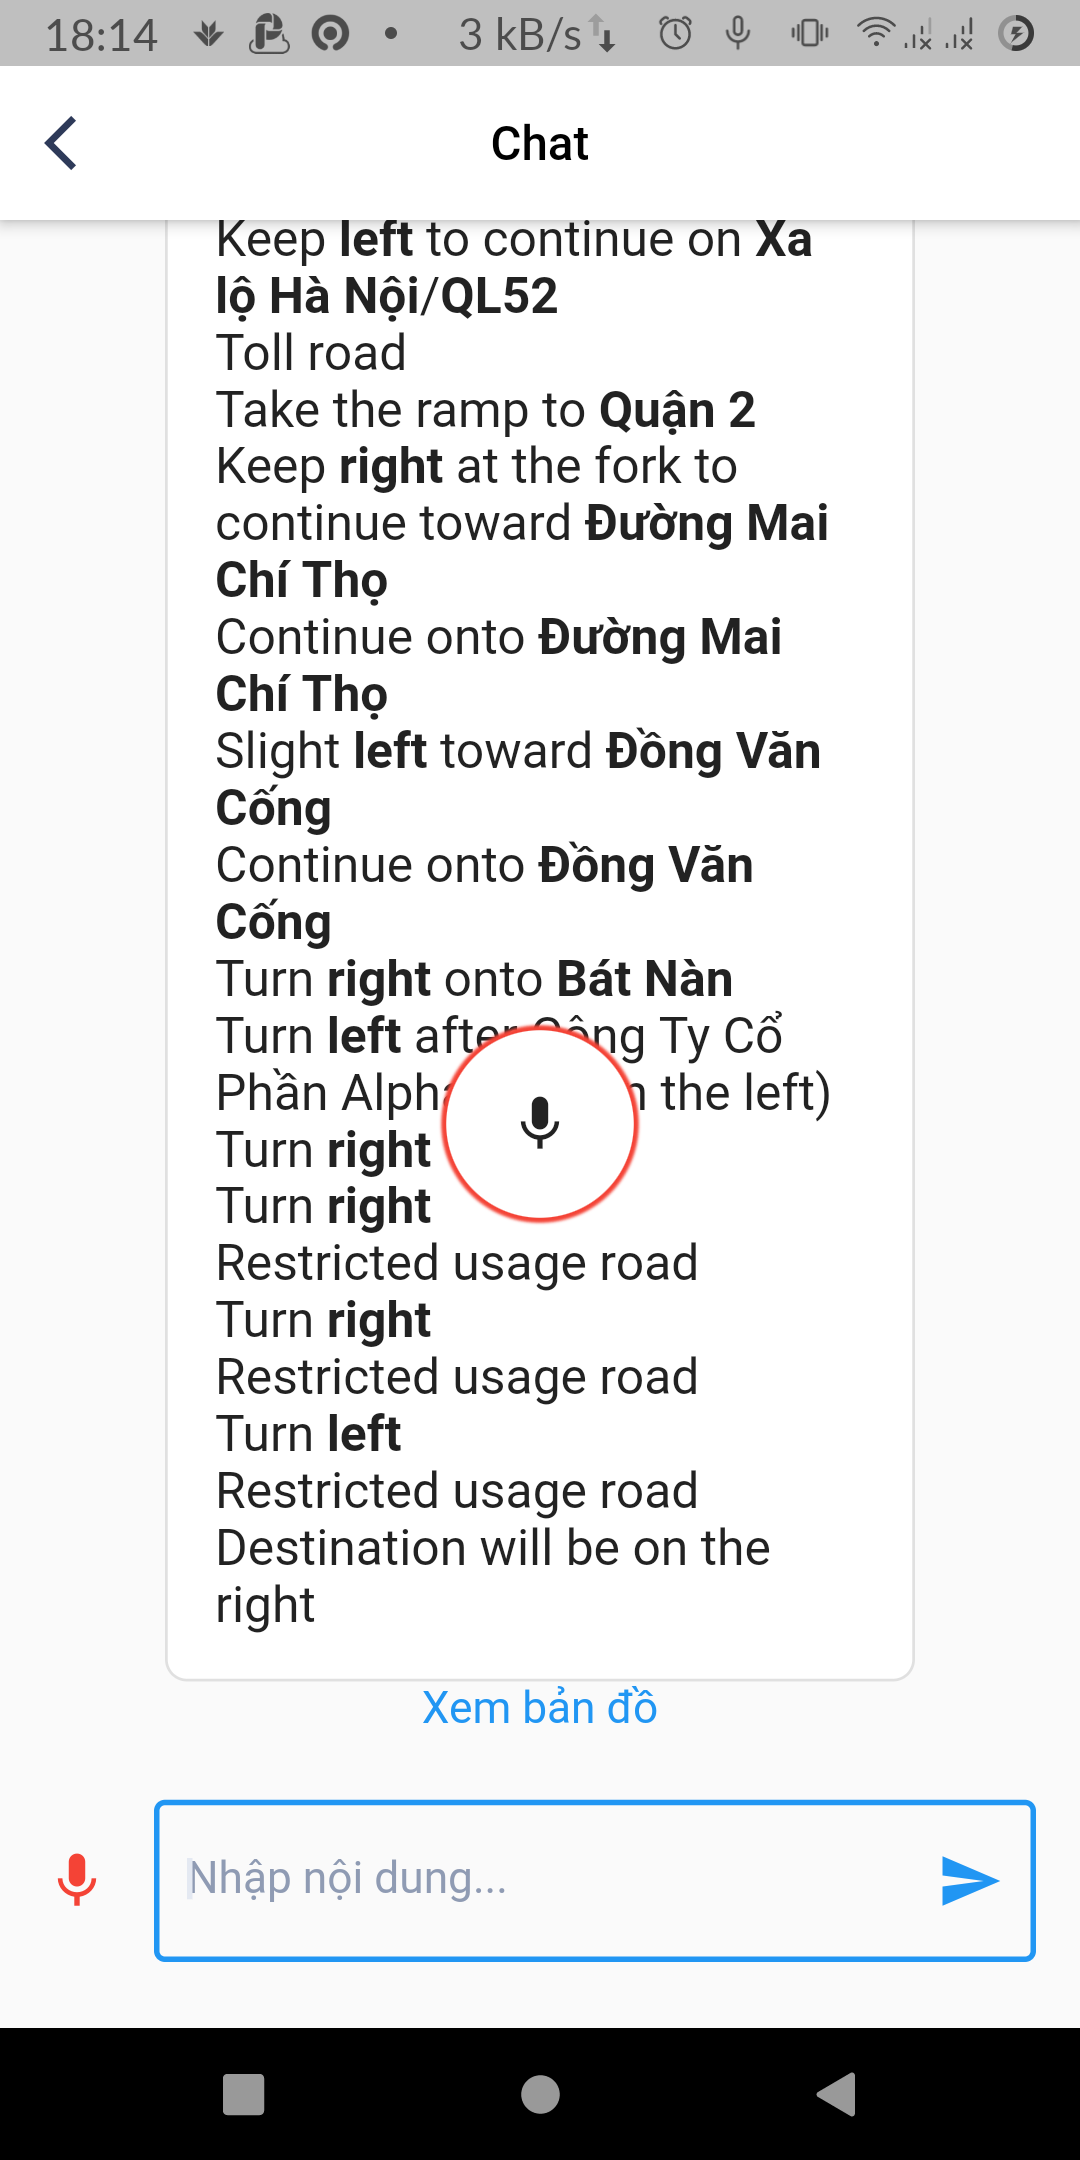
\includegraphics[width=5cm]{images/Screen-record.png}
    \caption{Màn hình thể hiện đang ghi âm}
    \label{fig:screen-record}
\end{figure}

Bán kính của vòng tròn hiển thị trong khi thực hiện quá trình ghi âm được hiển thị tăng giảm theo cường độ âm thanh thu được.

Sau khi kết thúc yêu cầu bằng giọng nói, ứng dụng tự động chuyển đổi giọng nói thành văn bản gửi lên hệ thống và hiển thị văn bản lên màn hình cuộc hội thoại.

\textbf{Giao diện chức năng hiển thị bản đồ:}

Nếu đây là lần đầu sử dụng ứng dụng với chức năng này, ứng dụng sẽ xin người dùng cấp quyền cho phép truy cập vào vị trí của thiết bị (xem hình \ref{fig: accesss-location}). Người dùng cần phải cho phép để ứng dụng có thể biết được vị trí để thuận tiện hơn cho quá trình sử dụng chức năng này của ứng dụng.

\begin{figure}[H]
    \centering
    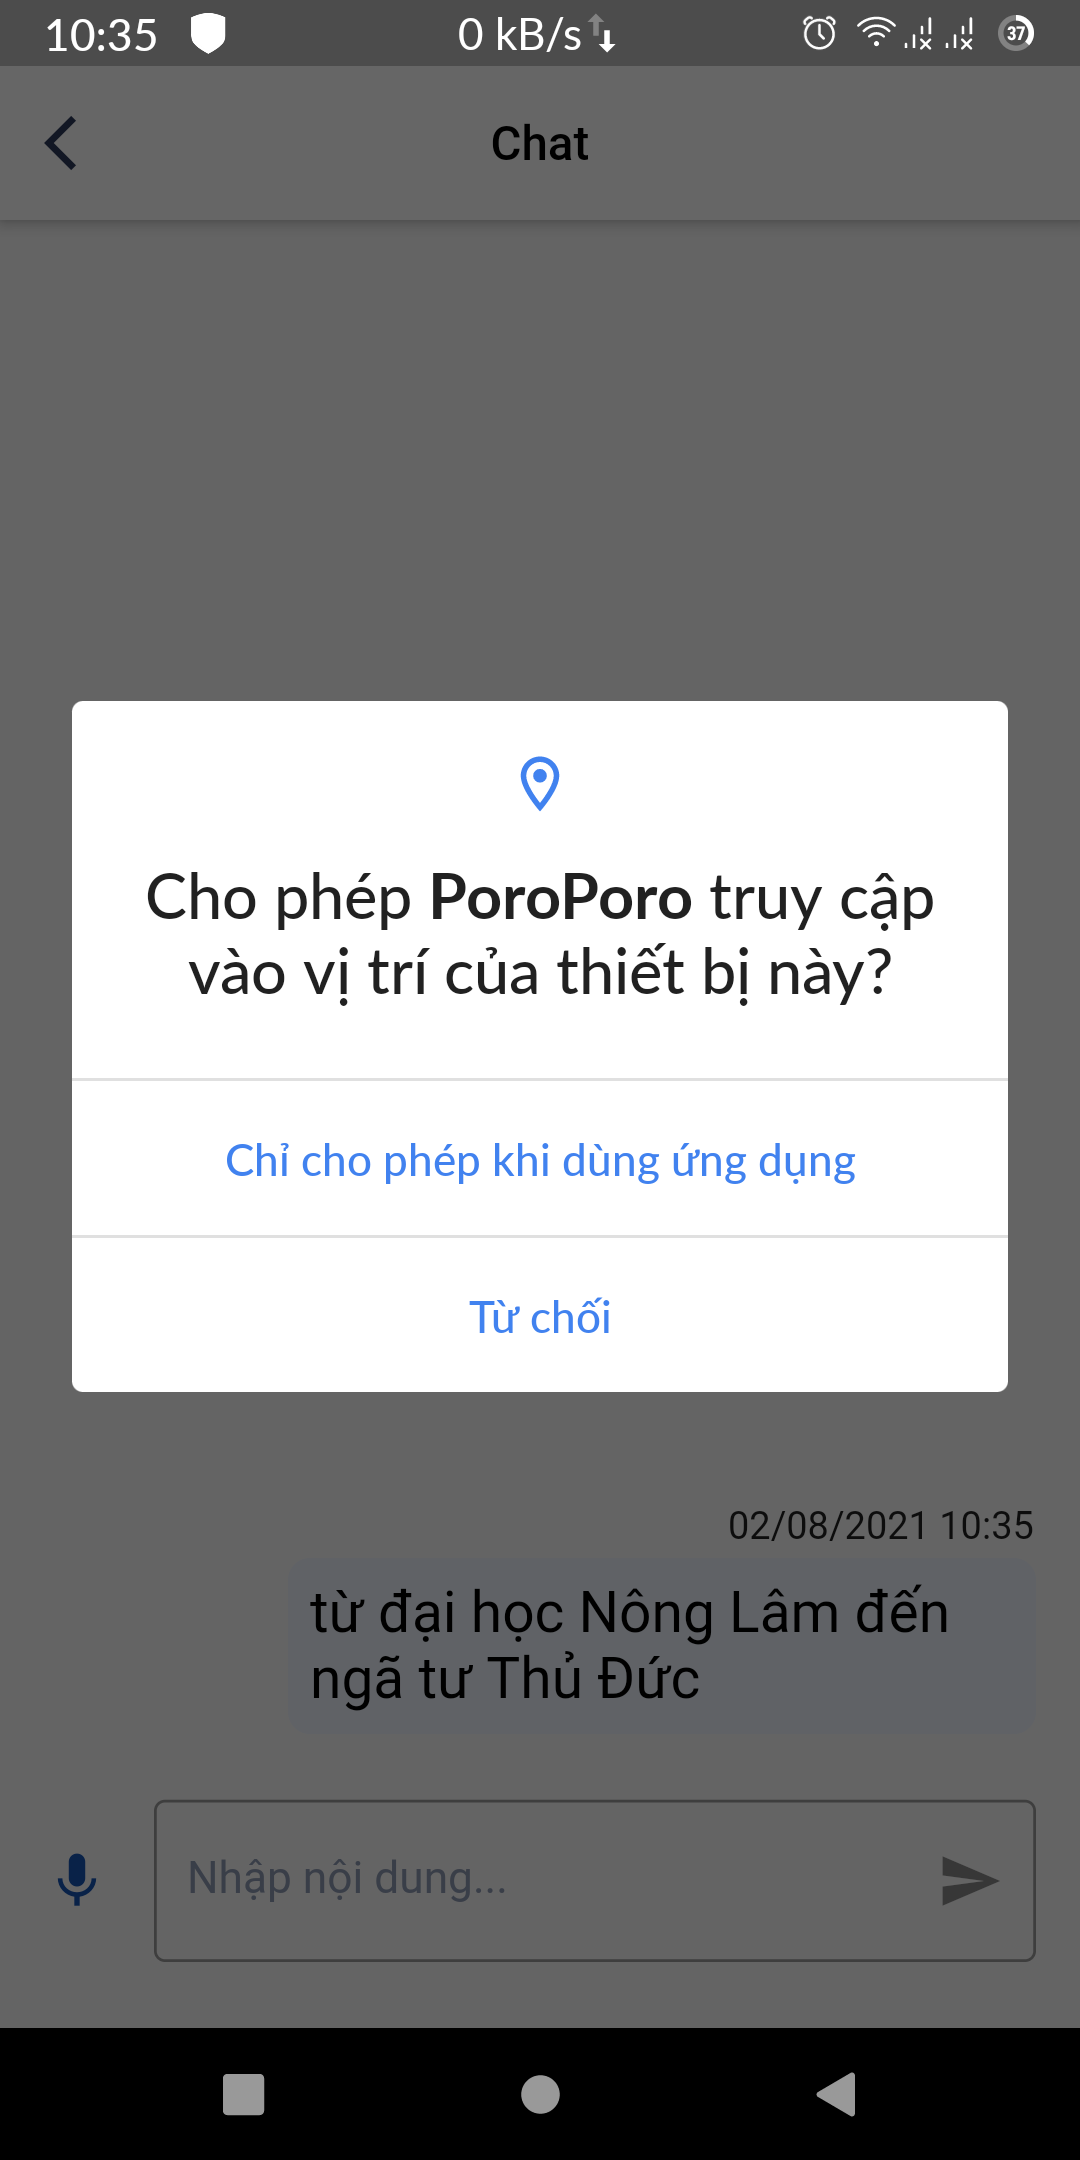
\includegraphics[width=5cm]{images/access_location.jpg}
    \caption{Màn hình xin quyền cấp phép truy cập vị trí hiện tại của thiết bị}
    \label{fig: accesss-location}
\end{figure}

Giao diện ứng dụng khi người dùng xem bản đồ đường đi trên ứng dụng (hình \ref{fig:screen-map}) :
\begin{figure}[H]
    \centering
    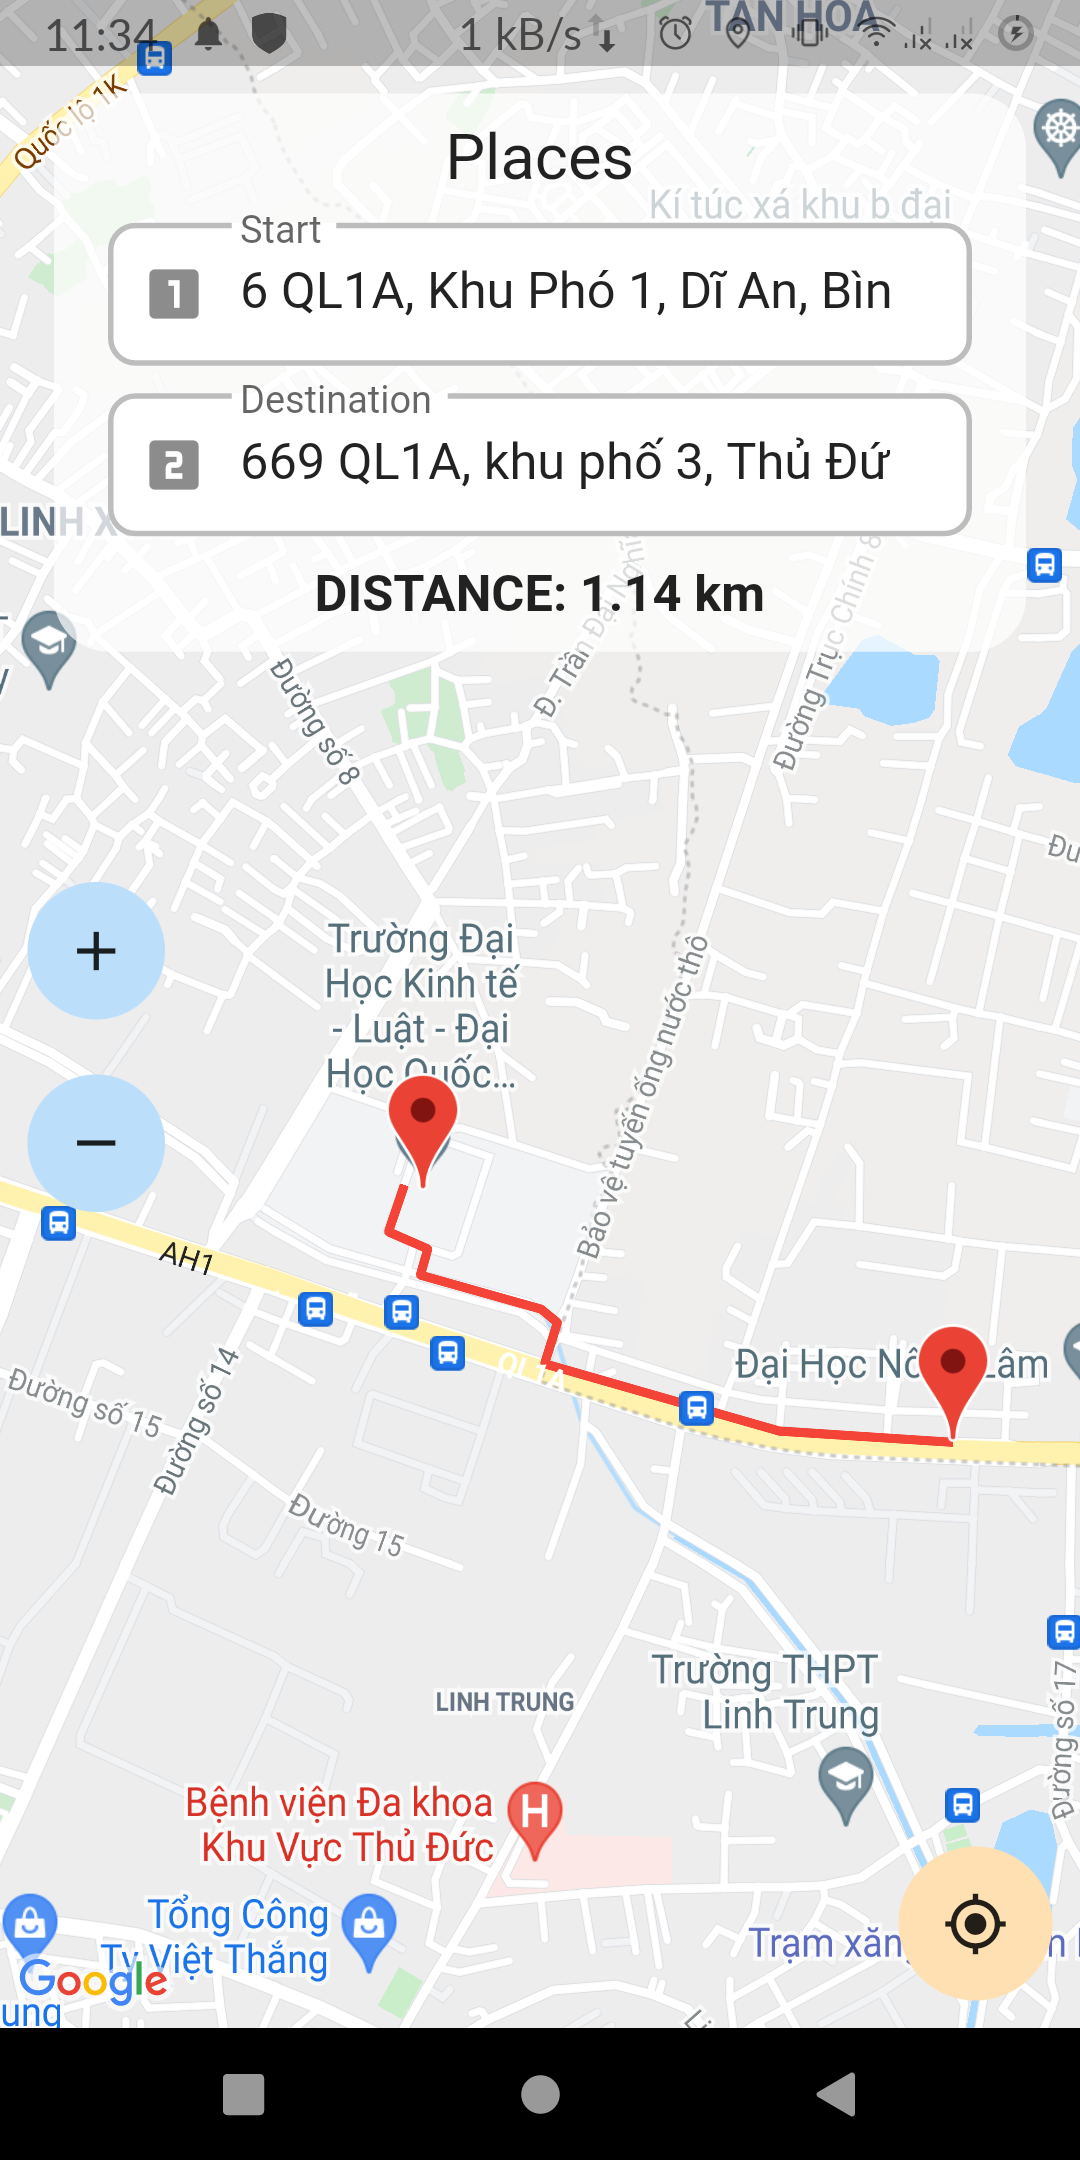
\includegraphics[width=5cm]{images/Screen-Map.png}
    \caption{Màn hình chỉ đường}
    \label{fig:screen-map}
\end{figure}

Giao diện gồm các phần sau đây:
\begin{itemize}
    \item[--] "Bắt đầu": Hiển thị thông tin địa điểm bắt đầu.
    \item[--] "Kết thúc": Hiển thị thông tin địa điểm kết thúc.
    \item[--] Hiển thị khoảng cách của hai địa điểm.
    \item[--] Chính giữa màn hình hiển thị bản đồ, điểm đầu và điểm cuối đường đi và đường đi giữa hai điểm được thể hiện bằng dòng kẻ màu đỏ.
    \item[--] Bên trái màn hình có button phóng to và thu nhỏ bản đồ.
    \item[--] Bên góc bên phải phía dưới màn hình có button dùng để xác định vị trí hiện tại của người dùng.
\end{itemize}

\chapter{Kết luận và Hướng phát triển}
\label{Chapter7}

\emph{Chương này trình bày kết luận sau quá trình thực hiện đề tài, bao gồm kỹ năng nghiên cứu, kỹ năng xây dựng một ứng dụng hoàn chỉnh, kết quả tóm tắt, ý nghĩa và khuyết điểm của đề tài. Cuối cùng là hướng phát triển và những định hướng trong tương lai.}

\section{Kết luận}
\label{sec:ket-luan}

\subsection{Tóm tắt kết quả đạt được}

Trong quá trình thực hiện khóa luận, nhóm em đã học hỏi và đạt được một số kết quả. Cụ thể:

\begin{itemize}
    \item[--] Về mặt nghiên cứu và ứng dụng:
        \begin{itemize}
            \item[\textbullet] Nghiên cứu phương pháp xác định ý định và trích xuất thực thể (Detect Intent \& Extract Entities) từ văn bản nhận được bằng cách ứng dụng thư viện mã nguồn mở Snips NLU. 
            \item[\textbullet] Nghiên cứu ứng dụng phương pháp chuyển đổi giọng nói thành văn bản và chuyển đổi văn bản thành giọng nói với bộ thư viện speech\_to\_text và flutter\_tts.  
            \item[\textbullet] Tìm kiếm đưa ra câu trả lời phù hợp (Search compatible response) bằng cách sử dụng Google Map API để tìm kiếm kết quả trả về phù hợp. 
            \item[\textbullet] Tạo bộ dữ liệu huấn luyện bao gồm 80 câu huấn luyện và 40 câu kiểm thử cho 4 loại ý định trong lĩnh vực tìm đường đi. 
            \item[\textbullet] Xây dựng thành công ứng dụng chatbot chỉ đường trong phạm vi Thành phố Thủ Đức, với giao diện đơn giản, dễ dàng sử dụng và ngôn ngữ sử dụng chính là tiếng Việt. 
            \item[\textbullet] Ứng dụng được xây dựng và phát triển trên cả hai nền tảng là Android và iOS.
        \end{itemize}
    \item[--] Về mặt kĩ năng mềm
        \begin{itemize}
            \item[\textbullet] Kỹ năng đọc tài liệu và phân tích vấn đề.
            \item[\textbullet] Kỹ năng nghiên cứu dự án.
            \item[\textbullet] Kĩ năng làm việc nhóm và phân chia công việc.
            \item[\textbullet] Kĩ năng trình bày và thuyết trình, viết báo cáo.
        \end{itemize}
\end{itemize}

\subsection{Ý nghĩa}
Bên cạnh những kết quả, việc hoàn thành đề tài Xây dựng giải pháp trả lời tự động (chatbot) bằng tiếng Việt cũng mang lại những ý nghĩa đáng kể:

\begin{itemize}
    \item[--] Kết quả của đề tài là minh chứng cho tính khả thi của đề tài.
    \item[--] Đề tài cũng chứng minh ý nghĩa của một chatbot trong đời sống. Với việc tồn tại một chatbot có khả năng nghe hiểu và phản hồi bằng giọng nói và văn bản bằng tiếng Việt, rất nhiều vấn đề sẽ trở nên đơn giản, dễ dàng hơn và giúp tiết kiệm thời gian cho người dùng.
\end{itemize}

\subsection{Những hạn chế, giới hạn}
Ứng dụng chatbot giọng nói bằng tiếng Việt hoạt động tương đối tốt. Tuy nhiên, vẫn còn nhiều mặt hạn chế nhất định như sau:
\begin{itemize}
    \item[--] Đối với vấn đền phân tích intent và trích xuất slot đôi khi vẫn còn nhầm lẫn và chưa được chính xác.
    \item[--] Đối với từ điển dịch tự tạo còn ít từ và nhiều hạn chế khi dịch.
    \item[--] Đối với vấn đề phân tích văn bản thành giọng nói còn hạn chế ngôn ngữ tiếng Việt trên iOS.
\end{itemize}

\section{Hướng phát triển}


Từ những hạn chế đã được nêu phần Kết luận \ref{sec:ket-luan}, trong tương lai, nhóm có những dự định bao gồm cải tiến thuật toán phân tích intent, trích xuất slot, dịch thuật và bổ sung thêm những chức năng, câu hỏi đa dạng khác ngoài những câu hỏi đơn giản như hiện tại. Cụ thể như:

Đối với vấn đề phân tích intent và trích xuất slot, nhóm sẽ tiếp tục tìm các giải pháp khác nhau để cải thiện độ chính xác khi phân tích dữ liệu. Bằng cách thực hiện huấn luyện mô hình nhiều hơn và đào sâu vào thuật toán để xem xét nguyên nhân cụ thể và đưa ra hướng giải quyết.

Đối với chức năng các câu hỏi chỉ dẫn, bổ sung thêm một số câu hỏi hữu ích khác như tra cứu các địa điểm quán ăn, cây xăng xung quanh vị trí hiện tại hay ở một khu vực nhất định, tìm nhiều đường đi khác nhau, hỏi và phân tích được vấn đề giao thông hiện tại như kẹt xe,... Và nâng cao hơn là áp dụng các mô hình xử lý ngôn ngữ tự nhiên để hệ thống có thể hiểu câu lệnh tốt hơn.


% In tài liệu tham khảo
\phantomsection
\addcontentsline{toc}{chapter}{Tài liệu tham khảo}
\printbibheading[title={Tài liệu tham khảo}]

\printbibliography[heading=subbibliography, title={Tiếng Việt}, keyword=Viet, resetnumbers=true]

\DeclareNameAlias{sortname}{family-given}
\DeclareNameAlias{default}{family-given}

\printbibliography[heading=subbibliography, title={Tiếng Anh}, notkeyword=Viet, resetnumbers=1]

\end{document}